\documentclass{report}

% Lecture Course Title and Lecturer
\newcommand{\coursetitle}{The Standard Model}
\newcommand{\lecturer}{Fernando Quevedo}
\newcommand{\term}{Lent}

% A shared preamble for the Part III Live-TeXing 2019

% Font
\usepackage[upint]{stix2}

% Graphics
\usepackage[dvipsnames]{xcolor}
\definecolor{Aqua}{rgb}{0.0, 1.0, 1.0}
\definecolor{CambridgeBlue}{RGB}{163, 193, 173}
\usepackage{graphicx}
\graphicspath{{lectures/}}
\usepackage{wrapfig}
\usepackage{keyval}
\usepackage[theorems]{tcolorbox}
\newtcolorbox{gatherbox}{colback=white, colframe=black, boxrule=0.5pt, sharp corners, ams gather}
\newtcolorbox{equationbox}{colback=white, colframe=black, boxrule=0.5pt, sharp corners, ams equation}
\newtcolorbox{alignbox}{colback=white, colframe=black, boxrule=0.5pt, sharp corners, ams align}
\usepackage{subcaption}
\usepackage{soul}
\usepackage{empheq}

\usepackage{tikz}
%\usetikzlibrary{calc}
\usepackage[compat=1.1.0]{tikz-feynman}
\usepackage{tikz-cd}

% Mathematical Symbols
\usepackage{amsmath}
\usepackage{mathtools}
\usepackage{physics} 
%\usepackage{amssymb} % made redundant by STIX2
\usepackage{mathrsfs}
\usepackage{cancel}
\usepackage{siunitx}
\usepackage{tensor}
\usepackage{bbold}
\usepackage{simpler-wick}
\usepackage[shortlabels]{enumitem}
\setlist[description]{leftmargin=\parindent,labelindent=\parindent}

% Links
\usepackage{hyperref}
\hypersetup{
  %hidelinks,
  pdfencoding=auto,
  pdfauthor={Umut \"Ozer},
  pdfsubject={\coursetitle{}},
  pdfcreator={Umut \"Ozer},
  pdfproducer={Umut \"Ozer},
  pdfkeywords={\coursetitle{},\term{},\lecturer{},Umut \"Ozer},
  colorlinks=true,
  linkcolor=MidnightBlue!50!BlueViolet,
  linktoc=all,
  urlcolor=blue,
}
\usepackage{bookmark} % faster updated bookmarks

% Page and Line Formatting
\setlength\parindent{1em}
\setlength{\parskip}{0.8em}
\usepackage[margin=35mm]{geometry}
\renewcommand{\baselinestretch}{1.3}

% Headers and Footers
\usepackage{fancyhdr}
\pagestyle{fancy}
\fancyhf{}
\chead{\coursetitle{}}
\rhead{Page \thepage}
%\lfoot{\leftmark}
%\rfoot{\rightmark}
\cfoot{\nouppercase\leftmark}
\renewcommand{\footrulewidth}{0.5pt}

% Chapter title formatting
%\renewcommand{\thechapter}{\Roman{chapter}}
\usepackage{titlesec}
\titleformat{\chapter}[hang]
{\normalfont\huge\bfseries}{\thechapter}{1em}{}

% Line Numbers (Pre-Publishing)
%\usepackage{lineno}
%\linenumbers

% Numbering by Section
%\usepackage{placeins}
%\let\Oldsection\section
%\renewcommand{\section}{\FloatBarrier\Oldsection}
%\let\Oldsubsection\subsection
%\renewcommand{\subsection}{\FloatBarrier\Oldsubsection}
%\let\Oldsubsubsection\subsubsection
%\renewcommand{\subsubsection}{\FloatBarrier\Oldsubsubsection}
%\numberwithin{equation}{chapter}
%\numberwithin{figure}{chapter}
%\numberwithin{table}{chapter}

%Footnotes
\usepackage{perpage}
\MakePerPage{footnote}

% Theorems and Definition
\usepackage{amsthm}
\newtheoremstyle{StandardStyle}% name of the style to be used
  {\topsep}% measure of space to leave above the theorem. E.g.: 3pt
  {\topsep}% measure of space to leave below the theorem. E.g.: 3pt
  {\normalfont}% name of font to use in the body of the theorem
  {}% measure of space to indent
  {\bfseries}% name of head font
  {:}% punctuation between head and body
  { }% space after theorem head; " " = normal interword space
  {}% Manually specify head
\theoremstyle{StandardStyle}

\newtheorem{theorem}{Theorem}
\newtheorem{lemma}[theorem]{Lemma}
\newtheorem{conjecture}{Conjecture}
\newtheorem{claim}{Claim}
\newtheorem*{proposition}{Proposition}
\newtheorem*{corollary}{Corollary}

\newtheorem{definition}{Definition}
\newtheorem*{notation}{Notation}

\newtheorem{example}{Example}[section]
\newtheorem{exercise}{Exercise}[chapter]

\usepackage{framed} % for \leftbar next to remark
\newtheorem*{remark}{Remark}
\newtheorem*{note}{Note}

% --- QUOTE ENVIRONMENT ---
% source: https://tex.stackexchange.com/questions/16964/block-quote-with-big-quotation-marks
\newcommand*\openquote{\makebox(25,-22){\scalebox{5}{``}}}
\newcommand*\closequote{\makebox(25,-22){\scalebox{5}{''}}}
\colorlet{shadecolor}{CambridgeBlue}

\makeatletter
\newif\if@right
\def\shadequote{\@righttrue\shadequote@i}
\def\shadequote@i{\begin{snugshade}\begin{quote}\openquote}
\def\endshadequote{%
  \if@right\hfill\fi\closequote\end{quote}\end{snugshade}}
\@namedef{shadequote*}{\@rightfalse\shadequote@i}
\@namedef{endshadequote*}{\endshadequote}
\makeatother

% differential (upright d):
\newcommand{\bdd}[2][]{\mathop{\mathrm{d\hspace*{-0.2em}\bar{}\hspace*{0.2em}}^{#1}\hspace*{-0.05em}{#2}}}

% bar delta
\newcommand{\bdelta}{\delta\hspace*{-0.2em}\bar{}\hspace*{0.2em}}

% definition of path integral measure
\newcommand*\pdd[1]{\mathop{\mathcal{D} #1}}

% normal ordering : A B C :
\newcommand{\normalorder}[1]{\mathop{:}\nolimits\!#1\!\mathop{:}\nolimits}

% Set delimiter | that resizes to \left\{ \right}:
\newcommand{\suchthat}{\ifnum\currentgrouptype=16 \;\middle|\;\else\mid\fi}

% Pfaffian
\newcommand{\Pf}[1]{\mathop{\text{Pfaff}\, #1}}

% Floor and Ceiling funciton
% NB: use \floor*{. . .} for resized brackets
\DeclarePairedDelimiter\ceil{\lceil}{\rceil}
\DeclarePairedDelimiter\floor{\lfloor}{\rfloor}

\usepackage{ifthen}
\makeatletter
\newcommand{\yearofterm}[1]{%
  \ifthenelse{\equal{#1}{Michaelmas}}
    {2019}
    {2020}%
}
\makeatother

\author{Report typos to: \href{mailto:uco21@cam.ac.uk}{\ul{uco21@cam.ac.uk}}\\More notes at: \href{https://uco21.user.srcf.net/notes}{\ul{uco21.user.srcf.net}}}
\title{{\Huge \coursetitle{}}\\
  Part III \term{} \yearofterm{\term} \\
Lectures by \lecturer{}}


\begin{document}

\maketitle
\tableofcontents

% Lecture files
\lhead{Lecture 1: 10 October 2019}
\chapter{Introducing Differential Geometry}%

Structure: will do only differential geometry (maths methods) in the first 12 lectures, first 4 weeks. Afterwards the connection to the physics will be made.
We will develop a mathematical language that allows us to write valid equations involving vectors, similar to dimensional analysis for physicists. The physics will be introduced with the action principle.

Extra book: ``Geometry, Topology, and Physics'' by Nakahara.

Office Hours: Friday $4 \rightarrow 5$ in B2.13

Extra stuff not examinable. Lectures are what matters.

\section{Manifolds}%
\label{sec:manifolds}

\begin{definition}[]
An \emph{$n$-dimensional manifold} $\mathcal{M}$ is a space that locally looks like $\mathbb{R}^n$.
More precisely, we require
\begin{enumerate}
  \item For each point $p \in \mathcal{M}$, there is a map $\phi \colon \mathcal{O} \to U$ where $\mathcal{O} \subset \mathcal{M}$ is an open set with $p \in \mathcal{O}$ and $U \subset \mathbb{R}^n$.
    We will think of $\phi(p) = (x^1(p), \dots, x^n(p))$ as coordinates on $\mathcal{O} \subset \mathcal{M}$.

    This map must be a \emph{homeomorphism}:
    \begin{enumerate}
      \item injective (or 1-1) $p \neq q \implies \phi(p) \neq \phi(q)$
      \item surjective (or onto) $\phi(\mathcal{O}) = U$\par
	These ensure that $\phi^{-1}$ exists.
      \item both $\phi$ and $\phi^{-1}$ are continuous
    \end{enumerate}
  \item If $\mathcal{O}_\alpha$ and $\mathcal{O}_\beta$ are two open sets with 
    \begin{equation}
      \phi_\alpha: \mathcal{O}_\alpha \to U_\alpha \text{ and } \phi_\beta: \mathcal{O}_\beta \to U_\beta
    \end{equation}
    then the \emph{transition functions} $\phi_\alpha \circ \phi^{-1}_\beta: \phi_\beta(\mathcal{O}_\alpha \cap \mathcal{O}_{\beta}) \to \phi_\alpha (\mathcal{O}_\alpha \cap \mathcal{O}_\beta)$ are smooth (ie.~infinitely differentiable).
    The $\phi_\alpha$ are called \emph{charts}. The idea is that there may be different ways to assign coordinates to a given point $p \in \mathcal{M}$.
    The collection of all charts is called an \emph{atlas}.
    We require that these coordinate systems are mutually compatible. This is depicted in Figure \ref{fig:manifold}.
\end{enumerate}
\end{definition}

% F1
\begin{figure}[tbhp]
  \centering
  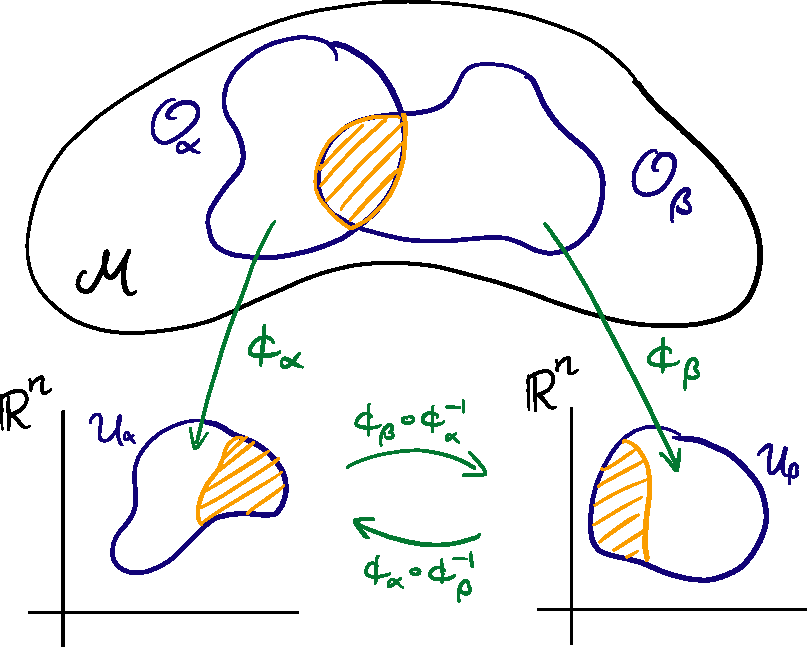
\includegraphics[width=0.5\linewidth]{lectures/F1.pdf}
  \caption{An illustration of charts on a manifold}
  \label{fig:manifold}
\end{figure}

\begin{example}[$\mathbb{R}^n$]
  $\mathbb{R}^n$ or any open subset of $\mathbb{R}^n$ is a manifold. You only need a single chart.
\end{example}

\begin{example}[$S^1$]
  We can view this as $(\cos \theta, \sin \theta) \in \mathbb{R}^{2}$ with $\theta \in [0, 2\pi)$. The closed set $[0, 2\pi)$ means that we cannot differentiate at $0$. This is \underline{not} a good chart because it is not an open set. 
  We need at least two charts, depicted in \ref{fig:L1F2}:
  \begin{equation}
    \begin{alignedat}{2}
      \phi_1 \colon \mathcal{O}_1 &\to (0, 2\pi)  \qquad&\qquad
      \phi_2 \colon \mathcal{O}_2 &\to (-\pi, \pi) \\
      p &\mapsto \theta_1 &
      p &\mapsto \theta_2
    \end{alignedat}
  \end{equation}
  The transition function is 
  \begin{equation}
    \theta_2 = \phi_2(\phi_1^{-1}(\theta_1)) = 
    \begin{cases}
      \theta_1, & \theta_1 \in (0, \pi) \\
      \theta_1 - 2\pi, & \theta_1 \in (\pi, 2\pi)
    \end{cases}
  \end{equation}
\begin{leftbar}
  \begin{remark}
    The fact that the coordinates go bad in the case of closed sets, similar to spherical polar coordinates, does not bother us too much for physical applications.
  \end{remark}
\end{leftbar}
\end{example}
\begin{figure}[htpb]
  \centering
  \def\svgwidth{0.7\columnwidth}
  \input{lectures/F2.pdf_tex}
  \caption{The two charts $\phi_1, \phi_2$ form an atlas of the manifold $S^1$.}
  \label{fig:L1F2}
\end{figure}

Since we can map $\mathcal{M} \to \mathbb{R}^n$ (at least locally), anything we can do on $\mathbb{R}^n$, we can now also do on $\mathcal{M}$ (e.g.~differentiation).

\begin{leftbar}
  \begin{remark}
    Note that at the moment, the distance in $\mathbb{R}^n$ cannot be translated back to the manifold. This is because the maps $\phi_\alpha$ are arbitrary.
  \end{remark}
\end{leftbar}

\begin{definition}[Diffeomorphism]
  A \emph{diffeomorphism} is a smooth homeomorphism $f: \mathcal{M} \to \mathcal{N}$ between two manifolds.
  I.e.~two manifolds are diffeomorphic if the map $\psi \circ f \circ \phi^{-1}: U \to V$ is smooth for \underline{all} charts $\phi: \mathcal{M} \to U \subset \mathbb{R}^n$ and $\psi: N \to V \subset \mathbb{R}^n$.
\end{definition}

\begin{leftbar}
  \begin{remark}
    There are interesting properties of $S^7$ and $\mathbb{R}^{4}$. You can find two atlasses of these manifolds such that the two atlasses are not diffeomorphic to each other.
    These are called \emph{exotic} manifolds; they are homeomorphic but not diffeomorphic to their respective Euclidean counterparts.
    As far as we know, there is yet no application of this in physics.
  \end{remark}
\end{leftbar}

\begin{leftbar}
  \begin{remark}
    These manifolds have intrinsic meaning and do not depend on an embedding. Physically, the $3+1$-dimensional spacetime is a manifold that we do not think is embedded in any higher dimensional space.
  \end{remark}
\end{leftbar}





% lecture notes by Umut Özer
% course: dgp
\lhead{Lecture 2: January 22}

\begin{definition}[surface]
  Let $f_1, \dots, f_k \colon \mathbb{R}^N \to \mathbb{R}$  be smooth functions.
  A surface $f_1 = 0, \dots, f_k = 0$  is a manifold of dimension $\dim n = N - k$ if the rank of the matrix  $\frac{\partial f_{\alpha}}{\partial x^{i}}$, $\alpha = 1, \dots, k$ and $i = 1, \dots, N$ is maximal and equal to $k$ at all points of $\mathbb{R}^N$..
\end{definition}
\begin{example}[]
  The $n$-sphere $S^n$ is a surface in $\mathbb{R}^{n+1}$ with $f_1 = 1 - \abs{\vb{r}}^2$.
\end{example}

\begin{theorem}[Whitney]
  Every smooth manifold of dimension $n$ is an embedded surface in $\mathbb{R}^N$, where $N \leq 2 n$.
\end{theorem}
\begin{leftbar}
  If you enjoy using geometrical intuition and looking at surfaces, this theorem ensures that you can always do that and not loose generality.
\end{leftbar}

\begin{definition}[real projective space]
  The $n$-dimensional \emph{real projective space} is defined as the quotient
  \begin{equation}
    \mathbb{RP}^n = (\mathbb{R}^{n+1} \setminus \{0\}) / \sim,
  \end{equation}
  where we quotient out the equivalence classes $[X_1, \dots, X_n+1] \sim [c X_1, \dots, cX_{n+1}]$ for all $c \in \mathbb{R}^*$.
  The $[X_1, \dots, X_{n+1}]$ are called \emph{homogeneous coordinates}.
\end{definition}
In other words, this is the space of all lines through the origin in $\mathbb{R}^{n+1}$ .

\begin{claim}
  $\mathbb{RP}^n$ is a smooth manifold of dimension $n$ with $(n+1)$ open sets.
\end{claim}
\begin{proof}
  Let us define our open sets with respect to the homogeneous coordinates.
  We define the set $U_{\alpha} \colon [X] \in \mathbb{RP}^n$  such that $X_{\alpha} \neq 0$  $\alpha = 1, \dots, n+1$ .
  We can now find local coordinates on $\phi_{\alpha} \colon U_{\alpha} \to V_{\alpha} \in \mathbb{R}^n$
  \begin{equation}
    x_1 = \frac{X_1}{X_{\alpha}} \quad \dots \quad x_{\alpha-1} = \frac{X_{\alpha-1}}{X_{\alpha}} \quad x_{\alpha+1} = \frac{X_{\alpha +1}}{X_{\alpha}} \quad \dots \quad x_n = \frac{X_n}{X_\alpha}.
  \end{equation}
\end{proof}
\begin{exercise}
  Prove smoothness of $\phi_{\beta} \circ \phi_{\alpha}^{-1}$.
\end{exercise}

\begin{figure}[tbhp]
  \centering
  \def\svgwidth{0.4\columnwidth}
  \input{lectures/l2f1.pdf_tex}
  \caption{Real projective space $\mathbb{RP}^n$ is isomorphic to $S^n / \mathbb{Z}^n$, identifying antipodal points.}
  \label{fig:l2f1}
\end{figure}

Now it turns out that this manifold is equivalent to $\mathbb{RP}^n = S^n / \mathbb{Z}^2$. From quantum mechanics, we know that this means in particular $\mathbb{RP}^3 = SO(3)$.
This is illustrated in \ref{fig:l2f1}.

\chapter{Vector Fields}%
\label{cha:vector_fields}

Let $M, \widetilde{M}$ be smooth manifolds of dimension $n, \tilde{n}$.

\begin{definition}[smooth map]
  A map $f\colon M \to \widetilde{M}$ is \emph{smooth} if $\widetilde{\phi}_{\beta} \circ f \circ \phi_{\alpha}^{-1}$ is a smooth map from $\mathbb{R}^n$ to $\widetilde{\mathbb{R}}^n$ for all $\alpha, \beta$.
  We call $f \colon M \to \mathbb{R}$ a \emph{function}, whereas we call $f\colon \mathbb{R} \to M$ a \emph{curve}.
\end{definition} 

Let $\gamma\colon \mathbb{R} \to M$ be a curve.
\begin{figure}[tbhp]
  \centering
  \def\svgwidth{0.4\columnwidth}
  \input{lectures/l2f2.pdf_tex}
  \caption{}
  \label{fig:l2f2}
\end{figure}
For some $U \in M$,  $U \simeq \mathbb{R}^n$ , we can define local coordinates $(x^1, \dots, x^n)$ .
% Missed something

\begin{definition}[tangent vector]
  A \emph{tangent vector} $V$  to $\gamma$ at  $p$ is 
   \begin{equation}
     V\rvert_p = \left. \dv{\psi}{\epsilon}\right\rvert_{\epsilon = 0} \in T_p M,
  \end{equation}
  where $T_p M$ is the \emph{tangent space} to $M$ at $p$.
\end{definition}
\begin{definition}[tangent bundle]
  We define the \emph{tangent bundle} as $T M \coloneqq \bigcup_{p \in M} T_p M$.
\end{definition}
\begin{definition}[vector field]
  A \emph{vector field} assigns a tangent vector to all $p \in M$ .
\end{definition}

Let $f\colon M \to \mathbb{R}$ . The rate of change of $f$  along $ \gamma$ is
\begin{align}
  \dv{}{\epsilon} f(x^{a}(\epsilon)) \rvert_{\epsilon =0} &= \sum_a \dot{x}^{a} \frac{\partial f}{\partial x^{a}} \\
						      &= \sum_a V^{a} \left. \frac{\partial f}{\partial x^{a}}\right\rvert_{\epsilon=0},
\end{align}
whee $V^{a} \coloneqq \dot{x}^{a}\rvert_{\epsilon=0, \dots, x_n}$.

Vector fields are first order differential operators
\begin{equation}
  V = \sum_a V^{a}(\vb{x}) \frac{\partial }{\partial x^{a}}.
\end{equation}
The derivatives $\left.\left\{ \frac{\partial }{\partial x^1}, \dots, \frac{\partial }{\partial x^{n}} \right\} \right\rvert_p$ form a basis of $T_p M$. 

\section{Integral curves}%
\label{sec:integral_curves}

\begin{definition}[integral curve]
  An \emph{integral curve} (a \emph{flow}) of a vector field is defined by
  \begin{equation}
    \dot{\gamma} (\epsilon) = V \rvert_{\gamma(\epsilon)},
  \end{equation}
  where the dot denotes differentiation with respect to $\epsilon$.
\end{definition}

On $n$  first order ODEs: $\dot{x}^{a} = V^{a} (x)$ .

There exists a unique solution given initial data $X^{a} (0)$ .
Given a solution $X^{a}(\epsilon)$ , we can expand it in a Taylor series as
\begin{equation}
  X^{a}(\epsilon) = X^{a}(0) + V^{a} \cdot \epsilon + O(\epsilon^2).
\end{equation}
Up to first order in $\epsilon$, the vector field determines the flow.
We call  $V$  a \emph{generator} of its flow.

The following example illustrates how you get from a vector field to its flow.
\begin{example}[$M = \mathbb{R}^2$, $x^{a} = (x, y)$]
  Consider the vector field $V = x \frac{\partial }{\partial x} + \frac{\partial }{\partial y}$ .
  The system of ODEs we solve is $\dot{x} = x$ and $\dot{y} = 1$ .
  This gives us the integral curve $(x(\epsilon), y(\epsilon)) = (x(0)e^\epsilon, y(0) + \epsilon)$ .
  From this we can see that $x(\epsilon) \cdot \exp(-y (\epsilon))$  is constant along $\gamma$.
  Using this we can draw the unparametrised integral curve in Fig.~\ref{fig:l2f3}.
   \begin{figure}[tbhp]
    \centering
    \def\svgwidth{0.4\columnwidth}
    \input{lectures/l2f3.pdf_tex}
    \caption{}
    \label{fig:l2f3}
  \end{figure}
\end{example}

This example motivates the following definition.
\begin{definition}[invariant]
  An \emph{invariant} of a vector field $V$ is a function $f$ constant along the flow of $V$.
  \begin{equation}
    f(x^{a}(0)) = f(x^{a}(\epsilon)) \qquad \forall \epsilon.
  \end{equation}
  Equivalently, $V(f) = 0$.
\end{definition}

Let us now consider an example that goes the other way: from flow to vector field.
\begin{example}
  Consider the $1$ -parameter group of rotations of a plane.
  \begin{equation}
    (x( \epsilon), y(\epsilon)) = (x_0 \cos\epsilon - y_0 \sin \epsilon, x_0 \sin \epsilon + y_0 \cos \epsilon).
  \end{equation}
  The associated vector field is
  \begin{equation}
  V = \left.\left( \frac{\partial y(\epsilon)}{\partial \epsilon} \frac{\partial }{\partial y} + \frac{\partial x(\epsilon)}{\partial \epsilon} \frac{\partial }{\partial x} \right)\right\rvert_{\epsilon = 0} = x \frac{\partial }{\partial y} - y \frac{\partial }{\partial y}.
  \end{equation}
\end{example}

Now you can add vector fields, but there is also another operation.
\begin{definition}[Lie bracket]
  A \emph{Lie bracket} $[V, W]$ of two vector fields $V, W$ is a vector field defined by
  \begin{equation}
    [V, W](f) = V(W(f)) - W(V(f)) \qquad \forall f.
  \end{equation}
\end{definition}
\begin{leftbar}
  This is indeed another vector field since the commutator of two first order operators is another first order operator.
\end{leftbar}

\begin{example}[]
  Let $V = x \frac{\partial }{\partial x} + \frac{\partial }{\partial y}$  and $W = \frac{\partial }{\partial x}$ . We then have $[V, W] = - W$.
\end{example}
\begin{leftbar}
  This is not always the case but sometimes the Lie bracket reproduces some of the vector fields. There is an interesting algebraic structure to this.
\end{leftbar}
\begin{definition}[Lie algebra]
  A \emph{Lie algebra} is a vector space $\mathfrak{g}$ with an anti-symmetric, bilinear operation $[\ ,\ ]\colon \mathfrak{g} \times \mathfrak{g} \to \mathfrak{g}$, called a \emph{Lie bracket}, which satisfies the \emph{Jacobi identity}
  \begin{equation}
    [V, [U, W]] + [W, [V, U]] + [U, [W, V]] = 0 \qquad \forall U, V, W \in \mathfrak{g}.
  \end{equation}
\end{definition}
\begin{leftbar}
  We will spend some time discussing this abstractly, but then focus on the Lie algebras of vector fields in the main part of this course.
\end{leftbar}

% lecture notes by Umut Özer
% course: aqft
\lhead{Lecture 3: January 23}

\section{Interacting Theory}%
\label{sec:interacting_theory}

We want to go beyond the free theory.
The way we are going to achieve this is by an expansion about the classical result $\hbar$.
The resulting integral will end up not being convergent.

\begin{claim}
  Integrals like
  \begin{equation}
    \int \dd[]{\phi} f(\phi) e^{- S / \hbar}
  \end{equation}
  do not have a Taylor expansion about $\hbar = 0$.
\end{claim}
\begin{proof}[Proof (Dyson)]
  If the expansion about $\hbar = 0$ existed for $\hbar > 0$, then in the complex plane, there must be some open neighbourhood of $\hbar$ in which the expansion converges.
  For $S(\phi)$ has a minimum, the integral is divergent if $\Re (\hbar)< 0$.
  Therefore, the radius of convergence cannot be greater than zero.
\end{proof}

So the $\hbar$-expansion is at best \emph{asymptotic}.
\begin{definition}[asymptotic]
  A series $\sum_{n = 0}^{\infty} c_n \hbar^n$  is asymptotic to a function $I(\hbar)$ if
  \begin{equation}
    \lim_{\hbar \to 0^+} \frac{1}{\hbar^N} \abs{I(\hbar) - \sum_{n=0}^N c_n \hbar^n} = 0.
  \end{equation} 
\end{definition}
\begin{notation}[]
  We write $I(\hbar) \sim \sum_{n=0}^{\infty} c_n \hbar^n$.
\end{notation}

The series misses out transcendental terms like $e^{-\frac{1}{\hbar^2}} \sim 0$ . However, these can evidently be important since obviously $e^{-\frac{1}{\hbar^2}} \neq 0$  for finite $\hbar$. These are called  \emph{non-perturbative contributions}. These become important in particular for non-Abelian gauge theories.

Take the $\phi$-fourth action for a real scalar
\begin{equation}
  S(\phi) = \underbrace{\frac{1}{2} m^2 \phi^2}_{\mathclap{S_0(\phi)}} + \underbrace{\frac{\lambda}{4!} \phi^4}_{\mathclap{S_1(\phi)}} \qquad 
  \begin{gathered}
    m^2 > 0 \\
    \lambda > 0.
  \end{gathered}
\end{equation}
Expand the exponential in the paritition function $Z$ about the minimum of $S(\phi)$, which is $\phi = 0$.
\begin{align}
  Z &= \int \dd[]{\phi} \exp[-\frac{1}{\hbar} \left( \frac{1}{2} m^2\phi^2 + \frac{\lambda}{4!}\phi^4 \right)]  \\
    &= \int \dd[]{\phi} e^{-S_0 / \hbar} \overbrace{\sum_{n=0}^\infty \frac{1}{n!} \left( -\frac{\lambda}{4! \hbar} \right)^n \phi^{4 n}}^{\mathclap{e^{- S_1 / \hbar}}}.
\end{align}

In order to make progress, we truncate the series to be able to swap the order of summation and integration. This misses out transcendental terms.
In the end, we end up with a series that is asymptotic to $Z$:
 \begin{equation}
   Z \sim \frac{\sqrt{2\hbar}}{m} \sum_{n=0}^N \frac{1}{n!} \left( - \frac{\hbar \lambda}{4! m^4} \right)^n 2^{2v} \int_{0}^\infty \dd[]{t} e^{-t} t^{2n + \frac{1}{2} - 1}, 
\end{equation}
where $t = \frac{1}{2\hbar} m^2 \phi^2$. We recognise the integral to be the Gamma function
\begin{equation}
  \int_{0}^\infty \dd[]{t} e^{-t} t^{2n + \frac{1}{2} - 1} = \Gamma(2 n + \frac{1}{2}) = \frac{(4n)! \sqrt{\pi}}{4^{2n} (2n)!}.
\end{equation}
The partition function is
\begin{equation}
  \label{eq:3-Z0}
  Z \sim \frac{\sqrt{2 \pi \hbar}}{m} \sum_{n=0}^N \left( - \frac{\hbar \lambda}{m^4} \right)^n \underbrace{\frac{1}{(4!) n!}}_{\mathclap{(a)}}\underbrace{\frac{(4n)!}{2^{2n} (2n)!}}_{\mathclap{(b)}}
\end{equation}
The factor on the right comes in part from (a) the Taylor expansion of the term $S_1(\phi) = (\phi)\frac{\lambda}{4!} \phi^4$ in the exponential and from (b) the number of ways of pairing the $4n$ fields of the $n$ copies of $\phi^4$.
Stirling's approximation allows us to write $n! \approx e^{n \ln n}$ .
The factor in the partition function then become
\begin{equation}
  \frac{(4n)!}{(4!)^n n! 2^{2n} (2n)!} \approx n!.
\end{equation}
We end up with factorial growth, signalling that the series is not convergent, but asymptotic!

\subsection{Diagrammatic Method}%
\label{sub:diagrammatic_method}

Let us now introduce a current $J$ to obtain the generating function
\begin{align}
  Z(J) &= \int \dd[]{\phi} \exp[-\frac{1}{\hbar} \left( S_0(\phi) + S_1 (\phi) + J \phi \right)] \\
       &= \exp[-\frac{\lambda}{4! \hbar} \left( \hbar \frac{\partial }{\partial J} \right)^4] \underbrace{\int \dd[]{\phi} \exp[-\frac{1}{\hbar} (S_0 + J \phi)]}_{\mathclap{Z_0 (J)}} \\
       &\stackrel{\eqref{eq:generating-function}}{\propto} \exp[-\frac{\lambda}{4! \hbar} \left( \hbar \frac{\partial }{\partial J} \right)^4] \exp(\frac{1}{2\hbar} J^T M^{-1} J), \qquad M = m^2 \\
       &\sim \sum_{V=0}^N \frac{1}{V!} \left[ -\frac{\lambda}{4! \hbar} \left( \hbar \frac{\partial }{\partial J} \right)^4 \right]^V 
       \sum_{P=0}^\infty \frac{1}{P!} \left( \frac{1}{2\hbar} \frac{J^2}{2 \hbar m^2} \right)^P \label{eq:3-star}.
\end{align}
This is called the \emph{double expansion}.
Diagrammatically, each of the $P$ propagators, represented by a line as in Fig.~\ref{fig:l3f1a}, give a factor of $M^{-1} = m^{-2}$.  We use a large filled circle at the end of a line to represent a source factor $J$.
Each of the $V$ factors $\left( \frac{\partial }{\partial J} \right)^4$, originating from the interaction term $S_1(\phi)$, are associated with a vertex as in Fig.~\ref{fig:l3f1b}. We use a small dot (or sometimes a small square) to mark a vertex.

\begin{figure}[tbph]
  \centering
  \begin{subfigure}[t]{0.5\textwidth}
    \centering
    \feynmandiagram[transform shape, scale=1][horizontal=a to b] {
      a [large, dot] -- [solid,  edge label=$m^{-2}$] b [large, dot],
    };
    \caption{Propagator with external sources $J$ at both ends.}
    \label{fig:l3f1a}
  \end{subfigure}%
  \begin{subfigure}[t]{0.5\textwidth}
    \centering
    $ \begin{gathered}
      \feynmandiagram[transform shape, scale=0.4][horizontal=a to b] {
        a -- v [small, dot] --b,
        c -- v -- d
      };
    \end{gathered} \quad \sim \quad
    -\lambda \left( \frac{\partial }{\partial J} \right)^4$ 
    \caption{Vertex}
    \label{fig:l3f1b}
  \end{subfigure}
  \caption{Components of the diagrammatic representation of the double series.}
  \label{fig:l3f1}
\end{figure}

Let us check that we reproduce the result \eqref{eq:3-Z0} for $Z(0)$.
For a term to be non-zero when $J=0$, we need the number of derivations to be equal to the number of source terms coming from the end of propagators. 
\begin{notation}[external sources]
  We denote by $E$ the number of external sources, which are left undifferentiated.
  For $P$ propagtors and $V$ vertices, the number of such sources is
  \begin{equation}
    E \coloneqq 2 P - 4 V.
  \end{equation}
\end{notation}
For $Z(0)$ we will require $E = 0$, whereas for $n$-point functions, we will want $E = n$.
The first non-trivial terms are $(V, P) = (1, 2), (2, 4), \dots$.
\begin{equation}
  Z(0) \propto 1 + \quad
  \begin{gathered}
    \mathclap{\feynmandiagram[transform shape, scale=0.5][small, horizontal=a to b] {
       a -- [loop, min distance=2cm, in=-135, out=-45] a -- [loop, min distance=2cm, in=135, out=45] a,
     };}
  \end{gathered} \quad
  + \
  \begin{gathered}
    \feynmandiagram[transform shape, scale=0.8][small, horizontal=a to b, layered layout] {
      a -- [half left] b -- [half left] a,
      a -- [half left, looseness=0.5] b -- [half left, looseness=0.5] a,
    };
  \end{gathered} \
  +\quad
  \mathclap{\begin{gathered}
     \feynmandiagram[transform shape, scale=0.5][small, vertical=a to b, layered layout] {
       a -- [loop, min distance=2cm, in=135, out=45] a -- [half left] b -- [loop, min distance=2cm, in=-135, out=-45] b,
       b -- [half left] a,
     };
   \end{gathered}}\quad
  +
  \begin{gathered}
    \quad \mathclap{\feynmandiagram[transform shape, scale=0.5][small, horizontal=a to b] {
       a -- [loop, min distance=2cm, in=-135, out=-45] a -- [loop, min distance=2cm, in=135, out=45] a,
     };
   } \qquad
     \mathclap{\feynmandiagram[transform shape, scale=0.5][small, horizontal=a to b] {
        a -- [loop, min distance=2cm, in=-135, out=-45] a -- [loop, min distance=2cm, in=135, out=45] a,
      };}\quad
  \end{gathered}
  + 
  O(V=3).
\end{equation}

\subsection{Symmetry Factors}%
\label{sub:symmetry_factors}

\begin{definition}[symmetry factor]
  The \emph{symmetry factor} $S$ is the number of ways of redrawing the unlabeled diagram, leaving it unchanged.
\end{definition}

\begin{definition}[pre-diagram]
  A \emph{pre-diagram} for a $(V, P)$ term in the double expansion is a collection of $V$ vertices and $P$ propagators, where the ends of the vertex lines are labeled by numbers and the ends of the propagators labelled by letters.
\end{definition}
We count the number of times each diagram appears in the double expansion by using such pre-diagrams.

\begin{example}[$V = 1$]
  Consider the first diagram with only a single vertex and two loops attached to it.
  \begin{figure}[tbhp]
    \centering
    \feynmandiagram[transform shape, scale=1][small, horizontal=a to b] {
      a [particle=\(1\)] -- v [small, dot] -- b [particle=\(3\)],
      c [particle=\(4\)] -- v -- d [particle=\(2\)],
    };
    \qquad
    \feynmandiagram[small, horizontal=a to b] {
      a [large, dot, label=180:\(a\)] -- b [large, dot, label=0:\(a'\)],
      c [large, dot, label=180:\(b\)] -- d [large, dot, label=0:\(b\)],
      b -- [draw=none] d,
      a -- [draw=none] c,
    };
    \caption{Pre-diagram of the $V = 1$ diagram with $P = 2$ loops.}
    \label{fig:l3f2}
  \end{figure}
  There are $A = 4!$ ways of matching the sources $a, a', b, b'$ to the derivatives at $1, 2, 3$, and $4$.
  This is cancelled by a $4!$ in the denominator $F = (V!) (4!)^V (P!) 2^P = 4! \cdot 2 \cdot 2^2$ of Eq.~\eqref{eq:3-Z0}.

  So the $(V, P)= (1, 2)$ diagram comes with a prefactor of $\frac{A}{F} = \frac{1}{8}$ (times $-\hbar \lambda m^{-4}$). 
\end{example}

In general, $S$ is given by the relation $\frac{A}{F} = \frac{1}{S}$, where $A$ is the number of ways of assigning the sources to the derivatives and $F$ the number of non-equivalent permutations of all vertices, each vertex's legs, all propagators, and their ends.
However, the symmetry of each particular graph is important: If the diagram has a particular symmetry, then some permutations in $F$ may be identical and have been double-counted.
For the above diagram, consider the pairing $(1a, 2a', 3b, 4b')$. Swapping $a \leftrightarrow a'$ and $1 \leftrightarrow 2$ gives exactly the same graph, so it should not be counted twice.

An alternative way to determine $S$ is to consider the actions, which leave invariant the unlabelled diagram.
These are called the automorphisms of the graph.
For $(1, 2)$, we can swap the direction of upper and lower loops ($2^2$) and also swap upper and lower loops ($2$). Therefore, we obtain $S = 2 \cdot 2^2 = 8$.

\begin{example}[basketball]
  Let us look at a slightly more complicated example.
  The \emph{basketball} diagram has the symmetry factor
  \begin{equation}
    \begin{gathered}
      \feynmandiagram[transform shape, scale=0.8][horizontal=a to b, layered layout] {
        a [dot] -- [half left] b [dot] -- [half left] a,
        a -- [half left, looseness=0.5] b -- [half left, looseness=0.5] a,
      };
    \end{gathered}
    \qquad S = 4! \cdot 2 = 48
  \end{equation}
  The pre-diagram associated to this is
  \begin{equation}
    \begin{gathered}
      \feynmandiagram[transform shape, scale=0.5][horizontal=a to b] {
        a [particle=\(1\)] -- c [small, dot] -- b [particle=\(2\)],
	e [particle=\(4\)] -- c -- f [particle=\(3\)],
      };
    \end{gathered}
    \quad
    \begin{gathered}
      \begin{tikzpicture}
	\begin{feynman}
	  \tikzfeynmanset{every vertex={large, dot}};
	  \vertex[label=180:$a$] (a);
	  \vertex[right=2cm of a, label=0:$b$] (b);
	  \vertex[label=180:$c$, below=0.5cm of a] (c);
	  \vertex[right=2cm of c, label=0:$d$] (d);
	  \vertex[label=180:$e$, below=0.5cm of c] (e);
	  \vertex[right=2cm of e, label=0:$f$] (f);
	  \vertex[label=180:$g$, below=0.5cm of e] (g);
	  \vertex[right=2cm of g, label=0:$h$] (h);
	
	  \diagram* {
	    (a) -- (b),
	    (c) -- (d),
	    (e) -- (f),
	    (g) -- (h),
	  };
	\end{feynman}
      \end{tikzpicture}
    \end{gathered}
    \quad
    \begin{gathered}
      \feynmandiagram[transform shape, scale=0.5][horizontal=a to b] {
        a [particle=\(5\)] -- c [small, dot] -- b [particle=\(6\)],
	e [particle=\(8\)] -- c -- f [particle=\(7\)],
      };
    \end{gathered}
  \end{equation}
  We can simply calculate $F = 2 \cdot (4!)^2 \cdot 4! \cdot 2^4 = 4^3 \cdot 2^{14}$ and from the pre-diagram we determine the ways to pair currents and derivatives
  \begin{equation}
    A = \underbrace{(2 \cdot 4)}_{\mathclap{a}} \underbrace{(4)}_{\mathclap{b}} \underbrace{(2 \cdot 3)}_{\mathclap{c}} \underbrace{(3)}_{\mathclap{d}} \underbrace{(2 \cdot 2)}_{\mathclap{e}} \underbrace{(2)}_{\mathclap{f}} \underbrace{(2 \cdot 1)}_{\mathclap{g}} \underbrace{(1)}_{\mathclap{h}} = 3^2 \cdot 2^{10}.
  \end{equation}.
  There are probably multiple ways to obtain this factor, but the reasoning here was as follows:
  For the letter $a$, we have a choice (factor 2) whether to connect to the left or the right vertex. In each case, we have $4$ numbers to connect to.
  Since the basketball shape has no loops, this means that $b$ has no choice in which vertex to use; it always has to be the one that we did not choose for $a$. For $b$ we only have a choice of $4$ numbers to connect to.
  For $c$, we again have a choice of two vertices, but only three remaining numbers (since the others are filled by $a$ or $b$). We proceed in the same way for the remaining letters.
  Thus $A / F = 1 / 48$.
\end{example}

For the other diagrams, we have
\begin{equation}
  \frac{Z(0)}{Z_0(0)} = 1 - \frac{\lambda \hbar}{8 m^4} + \frac{\hbar^2 \lambda^2}{m^8} \left( \frac{1}{48} + \frac{1}{16} + \frac{1}{128} \right)
\end{equation}

% lecture notes by Umut Özer
% course: symmetries
\lhead{Lecture 4: October 17}

\begin{claim}
  Consider the matrix eigenvalue equation
  \begin{equation} \label{eq:evalue}
    M \vb{v}_\lambda = \lambda \vb{v}_\lambda,
  \end{equation}
  where $M \in O(n)$, the two defining properties of the orthogonal group are then that
  \begin{enumerate}
    \item If $\lambda$ is an eigenvalue, then its complex conjugate $\lambda^*$ is an eigenvalue as well.
    \item The eigenvalues are normalised such that $\abs{\lambda}^2 = 1$.
  \end{enumerate}
\end{claim}
\begin{proof}
  \begin{enumerate}
    \item Complex conjugating both sides of \eqref{eq:evalue} gives
      \begin{equation}
        M \vb{v}_\lambda^* = \lambda^* \vb{v}_\lambda^*
      \end{equation}
    \item First, note that we have \((M \vb{v}^*)^T \cdot M \vb{v} = \vb{v}^{\dagger} M^T M \vb{v} = \vb{v}^{\dagger} \cdot \vb{v}\).
      Then, if $\vb{v} = \vb{v}_\lambda$:
      \begin{equation}
	(M \vb{v}_\lambda^*)^T \cdot M \vb{v}_\lambda = \abs{\lambda}^2 \vb{v}^{\dagger}_\lambda \vb{v}_\lambda = \vb{v}^{\dagger}_\lambda \vb{v}_\lambda \implies \abs{\lambda}^2 = 1.
      \end{equation}
  \end{enumerate}
\end{proof}

\begin{example}[$SO(2)$]
  Let $M$ be a matrix in $SO(2)$. Then $M$ has eigenvalues $\lambda = e^{i\theta}, e^{-i\theta}$ for small $\theta \in \mathbb{R}$, with the identification $\theta \sim \theta + 2\pi$.
  In a matrix representation, we write
  \begin{equation}
    M = M(\theta) = 
    \begin{pmatrix}
     \cos\theta & -\sin\theta \\
     \sin\theta & \cos\theta \\
    \end{pmatrix}.
  \end{equation}
  Although this is a real matrix, its eigenvalues are complex. Provided that we made the identification $\theta \sim \theta + 2\pi$, the matrix is uniquely specified by $\theta$.
  Therefore, the manifold of this Lie group is $M(SO(2)) \cong S^1$.
  Moreover, since the matrices are commutative, $M(\theta_1) M(\theta_2) = M(\theta_2) M(\theta_1) = M(\theta_1 + \theta_2)$, this is an Abelian Lie group.
\begin{leftbar}
  \begin{remark}
    This is in fact the simplest compact Lie group.
  \end{remark}
\end{leftbar}
\end{example}

\begin{example}[$SO(3)$]
  We consider now matrices $M$ in the three-dimensional special orthogonal group $SO(3)$. The eigenvalues are $\lambda = e^{+i \theta}, e^{-i\theta}, +1$, where we again have made the identification $\theta \sim \theta + 2\pi$.
  To parametrise a rotation matrix in three dimensions, consider the normalised eigenvector corresponding to the  $\lambda = +1$ eigenvalue:
  \begin{equation}
    \hat{\vb{n}} \in \mathbb{R}^3, \qquad M \hat{\vb{n}} = \hat{\vb{n}}, \qquad \hat{\vb{n}} \cdot \hat{\vb{n}} = 1.
  \end{equation}
  The direction of $\hat{\vb{n}}$ parametrises the axis, and $\theta$ parametrises the angle of rotation.

  \begin{exercise}
    One can write a general group element of SO(3) as
    \begin{equation}
      M(\hat{\vb{n}}, \theta)_{ij} = \cos\theta \delta_{ij} + (1 - \cos\theta) n_i n_j - \sin\theta \varepsilon_{ijk} n_k.
    \end{equation}
  \end{exercise}

  We want to specify the elements uniquely. Above, one needs to be careful about the uniqueness, due to two issues:
  \begin{enumerate}
    \item Identification: $M(\hat{\vb{n}}, 2\pi - \theta) = M(-\hat{\vb{n}}, \theta)$
    \item If $\theta = 0$, then for all directions $\hat{\vb{n}}$, we have $M(\hat{\vb{n}}, 0) = I_3$,
  \end{enumerate}

  To be precise, we need to identify these rotations. To get a better parametrisation, define the parameter $\boldsymbol\omega = \theta \hat{\vb{n}}$.
  Consider the ball $B_3 \subset \mathbb{R}^3 = \left\{ \boldsymbol\omega \in \mathbb{R}^3 \mid \abs{\boldsymbol\omega} \leqslant \pi \right\}$.
  The group manifold associated with SO(3) is obtained by taking $B_3$ and identifying antipodal points on the boundary.

  \begin{figure}[tbph]
    \centering
    \begin{subfigure}[t]{0.3\linewidth}
      \centering
      \def\svgwidth{0.8\columnwidth}
      \input{lectures/ball.pdf_tex}
      \caption{The ball $B_3$ with radius $\pi$.}
      \label{fig:ball}
    \end{subfigure}\qquad
    \begin{subfigure}[t]{0.6\linewidth}
      \centering
      \def\svgwidth{\columnwidth}
      \input{lectures/identification.pdf_tex}
      \caption{Identifying opposing edges of a sheet of paper gives a space topologically equivalent to a torus.}
      \label{fig:identification}
    \end{subfigure}
    \caption{The group manifold associated with SO(3) is obtained by identifying antipodal points on the boundary $\partial B$ of the ball $B_3$.}
  \end{figure}

  \begin{leftbar}
    \begin{remark}
      In general, freely acting quotients give a manifold. Here, the group we quotiented out is the group of inversion $\mathbb{R}_2$.
    \end{remark}
  \end{leftbar}

  The resulting manifold is connected, but not simply connected. This is because loops that come out and back via the identification cannot be contracted to a point; antipodal points are always antipodal. This is illustrated in Figure~\ref{fig:antipodal_loops}.
  As such, we have $\pi_1(SO(3)) \neq \left\{ 0 \right\}$. In fact, the fundamental group is
  \begin{equation}
    \label{eq:so3-fund}
    \pi_1(SO(3)) \simeq \mathbb{Z}_2 = \left\{ +1, -1 \right\}.
  \end{equation}
  \begin{figure}[bhtp]
    \centering
    \def\svgwidth{0.25\columnwidth}
    \input{lectures/antipodal.pdf_tex}
    \caption{Loops passing through the identification of antipodal points cannot be contracted to a point. Note that the purple loop is constructible. This can be seen by ``rotating'' one half of the loop until it matches up with the other.}
    \label{fig:antipodal_loops}
  \end{figure}
\end{example}

\subsection*{The Unitary Groups}%

\begin{definition}[unitary group]
  The \emph{unitary group} $U(n)$ is the set of invertible complex matrices obeying $U^{\dagger} = U^{-1}$:
  \begin{equation}
    U(n) \coloneqq \left\{ U \in GL(n, \mathbb{C}) \mid U^{\dagger} U = I_n \right\}.
  \end{equation}
\end{definition}

\begin{claim}
  Let $U \in U(n)$ be a matrix in the unitary group. Under such a unitary transformation, the length of a vector $\vb{v}$ is unchanged.
\end{claim}
\begin{proof}
  The vector $\vb{v}$ transforms as \(\vb{v} \in \mathbb{C}^n \to \vb{v}' = U \vb{v} \in \mathbb{C}^n \).
  Using the property $U U^{\dagger} = 1_n$ of unitary matrices, we have
  \begin{equation}
    \abs{\vb{v}'}^2 = \vb{v}'^{\dagger} \cdot \vb{v}' = (\vb{v}^{\dagger} U^{\dagger}) \cdot (U \vb{v}) = \vb{v}^{\dagger} \cdot \vb{v} = \abs{\vb{v}}^2
  \end{equation}
\end{proof}

\begin{claim}
  Let $U \in U(n)$ be an element of the group of unitary $n \times n$ matrices. Then $\det U = e^{i\delta}$, where $\delta \in \mathbb{R}$.
\end{claim}
\begin{proof}
  $U^{\dagger}U = 1_n \implies \abs{\det U}^2 = 1 \implies \det U = e^{i\delta}$, $\delta \in \mathbb{R}$.
\end{proof}
\begin{leftbar}
  \begin{remark}
    Since $\delta \in \mathbb{R}$ is able to vary continuously, $U(n)$ is connected, whereas $O(n)$ was not.
  \end{remark}
\end{leftbar}

\begin{definition}[special unitary group]
  The \emph{special unitary group} $SU(n)$ is the subset of $U(n)$ with unit determinant:
  \begin{equation}
    SU(n) = \left\{ U \in U(n) \mid \det U = 1 \right\}
  \end{equation}
\end{definition}

\begin{claim}
  The groups $U(n)$ and $SU(n)$ are indeed Lie groups $\subset GL(n, \mathbb{C})$. Their dimensions are given by
  \begin{equation}
    \dim(U(n)) = 2n^2 - n^2 = n^2, \qquad \dim(SU(n)) = n^2 -1.
  \end{equation}
\end{claim}
\begin{proof}
  To see this, take any matrix $M \in \text{Mat}(n, \mathbb{C}) \leftrightarrow \mathbb{R}^{2n^2}$ (real and complex components) and apply the embedding theorem.
  The constraint for $U(n)$ is  $\mathcal{F} = U U^{\dagger} - I = 0$. This gives quadratic constraints in the matrix elements. Since $H = U U^{\dagger}$ is Hermitian, these are actually $n^2$ constraints instead of $2n^2$.
  For $SU(n)$, we require $\mathcal{F} = \det U - 1 = 0$. Since $\det U = e^{i\varphi}$, this is only one additional constraint.
\end{proof}

\subsection{Non-Compact Subgroups of \texorpdfstring{$GL(n, \mathbb{R})$}{GL(n, R)}}%
\label{sub:non_compact_subgroups_of_gl_n_r}

Orthogonal matrices obey $M M^T = I_n$. We can also read this as $M I_n M^T = I_n$; orthogonal transformations preserve the Euclidean metric $g = \text{diag}\underbrace{(1, \cdots, 1)}_{n \text{ times}}$ on $\mathbb{R}^n$.

We can generalise this by defining $O(p, q)$ to be the set of transformations that preserve the metric of signature $p, q$ :
\begin{equation}
  O(p, q) = \big\{ M \in GL(n, \mathbb{R}) \mid M^T \eta M = \eta, \text{where } \eta = \text{diag}(\underbrace{-1, \ldots, -1}_{p \text{ times}}, \underbrace{+1, \ldots, +1}_{q \text{ times}}) \big\}.
\end{equation}
In general, the manifolds of $O(p, q)$ are not compact.

\begin{example}[]
  The elements of $SO(2)$ are matrices of the form
  $ \begin{pmatrix}
   \cos\theta & -\sin\theta \\
   \sin\theta & \cos\theta \\
  \end{pmatrix} $
  , with the identification $\theta \sim \theta + 2\pi$. This identification means that as manifolds, $SO(2) \simeq S^1$, which is compact.

  In contrast to this, elements of $SO(1, 1)$ are matrices of the form
  $ \begin{pmatrix}
   \cosh\varphi & -\sinh\varphi \\
   \sinh\varphi & \cosh\varphi \\
  \end{pmatrix}
  $, where $\varphi$ is free to take any value $\varphi \in \mathbb{R}$. This means that the manifold of $SO(1, 1)$ is $\mathbb{R}$, which is evidently non-compact.
\end{example}

% lecture notes by Umut Özer
% course: bh
\lhead{Lecture 5: January 27}

\begin{definition}[]
  A \emph{solar mass black hole} has a mass $M \lesssim 100 M_\odot$. These are formed by the gravitational collapse of a star.
\end{definition}

\begin{figure}[tbhp]
  \centering
  \def\svgwidth{0.4\columnwidth}
  \input{lectures/l5f1.pdf_tex}
  \caption{}
  \label{fig:l5f1}
\end{figure}
Approximate disc particles as following circular orbits.

As the energy decreases (say by friction), the radius slowly decreases.
A particle from the disc reaches the ISCO. If it has energy $E = \sqrt{8 / 9}$ it falls into the hole.
A fraction of $1 - \sqrt{8 /9} \approx 6\%$ of the rest mass is lost to friction. This colossal amount of energy is converted to electromagnetic radiation.

\section{White Holes}%
\label{sec:white_holes}

Consider the $r > 2M$ Schwarzschild solution.
\begin{definition}[outgoing EF coords]
  Now define $u \coloneqq t - r_*$, which is constant along \emph{outgoing} radial null geodesics.
  Then $(u, r, \theta, \phi)$ define \emph{outgoing Eddington--Finkelstein coordinates}.
\end{definition}
The metric in these coordinates is
\begin{equation}
  ds^2 = - \left( 1 - \frac{2M}{r} \right) du^2 - 2du dr + r^2 d\Omega^2.
\end{equation}

Just as in the ingoing case, we can extend this though $r = 2M$ to  $r \leq 2M$  until the curvature singularity at $r = 0$.
 \begin{claim}
  This is not the same as the previous $r \leq 2M$ region!
\end{claim}
\begin{proof}
  Consider for example the outgoing radial null geodesics $u = \text{const.}$  and $\dv{r}{\tau} = +1$ .
  In this $r < 2M$ region, $r$ is increasing, so it cannot be the same region as before.
\end{proof}
\begin{exercise}
  Repeat the calculation as for the ingoing case to show $k = \frac{\partial }{\partial u}$ in ingoing EF coordinates and $\frac{\partial }{\partial r}$  is the time-orientation equivalent to $k$ in $r > 2M$.
\end{exercise}
\begin{leftbar}
  The fundamental confusion of calculus: $\frac{\partial }{\partial r}$  in the ingoing coordinates is not the same as in the outgoing coordinates, since we are holding different coordinates fixed.
\end{leftbar}

\begin{definition}[white hole]
  A \emph{white hole} is a region that cannot receive a signal from $\infty$.
\end{definition}

The $r \leq 2M$  region is a \emph{white hole}!

A white hole is essentially a time-reverse of a black hole.
If we substitute $u = -v$ , we recover the metric from the ingoing coordinates.
Therefore, $u = -v$  is an isometry mapping the white hole to the black hole, which reverses the time orientation.

White holes are unphysical\footnote{As discussed in \emph{General Relativity}, our universe (emerging from the big bang singularity) looks a bit like the inside of a white hole in $5$ dimensions.}, since there is no mechanism for forming them; you would have to start with the singularity at $r = 0$ and get the white hole emerging from it.
Black holes are stable; small perturbations will decay. Since white holes are time-reversals of black holes, they are unstable objects. 

\section{Kruskal Extension}%
\label{sec:kruskal_extension}

\begin{definition}[]
  For $r > 2M$, take the \emph{Kruskal--Szekeres} coordinates $(U, V, \theta, \phi)$ with $0> U = -e^{-u / 4M}$ and $0< V = +e^{v / 4M}$.
\end{definition}

We then have
\begin{equation}
  UV = -e ^{r_* / 2M} = -e^{r / 2M} (\frac{r}{2M} - 1) \label{eq:5-star}.
\end{equation}
The right hand side is monotonic. Therefore, if we know $U$  and $V$ , we can determine $r = r(U, V)$  uniquely.
Similarly, 
\begin{equation}
  \frac{V}{U} = -e^{t / 2M}
\end{equation}
fixes $t (U, V)$ .
\begin{exercise}
  Show that in these coordinates the metric is
  \begin{equation}
    ds^2 = -\frac{32M^3}{ r(U, V)} e^{-r(U, V) / 2M} dU dV + r(U, V)^2 d\Omega^2.
  \end{equation}
\end{exercise}
We can smoothly extend this metric to a larger range of $U$ and  $V$ , since it remains smooth and invertible.
We can now use \eqref{eq:5-star} to define $r(U, V)$  for $U \geq 0$  or $V \leq 0$ . The metric can then be analytically extended with $\det g_{\mu\nu} \neq 0$  to new regions, where either $U > 0$ or  $V < 0$. 

What does the Schwarzschild radius $r = 2M$ correspond to?
We have  $U V = 0$, which corresponds either to  $U = 0$ or  $V = 0$. In fact, this is not one surface but two!

What about the curvature singularity at  $r = 0$?
Equation  \eqref{eq:5-star} gives $UV = 1$, a hyperbola.
 \begin{figure}[tbhp]
  \centering
  \def\svgwidth{0.8\columnwidth}
  \input{lectures/l5f2.pdf_tex}
  \caption{Kruskal diagram}
  \label{fig:l5f2}
\end{figure} 
Radial null geodesics correspond to constant $U$  or $V$.

We have four regions
 \begin{enumerate}[I:]
  \item $r > 2M$ Schwarzschild
  \item Black hole region
  \item White hole region
  \item new region with $r > 2M$ isometric to $I$ via $(U, V) \to (-U, -V)$
\end{enumerate}
\begin{leftbar}
  Ingoing EF cover I and II, while outgoing EF cover I and III.
\end{leftbar}

\begin{figure}[tbhp]
  \centering
  \begin{minipage}[t]{0.5\textwidth}
    \centering
    \def\svgwidth{0.8\columnwidth}
    \input{lectures/l5f3.pdf_tex}
    \caption{A star collapsing to form a black hole. The interior of the star covers up III and IV.}
    \label{fig:l5f3}
  \end{minipage}%
  \begin{minipage}[t]{0.5\textwidth}
    \centering
    \def\svgwidth{0.8\columnwidth}
    \input{lectures/l5f4.pdf_tex}
    \caption{Orbits (integral curves) of $k$.}
    \label{fig:l5f4}
  \end{minipage}
\end{figure}


\begin{exercise}
  Show 
  \begin{equation}
    k = \frac{1}{4M} \left( V \frac{\partial }{\partial V} - U \frac{\partial }{\partial U} \right) \qquad k^2 = - \left( 1 - \frac{2M}{r} \right),
  \end{equation} 
  timelike in I, IV, spacelike in II, III, and null at $U = 0$ or $V = 0$.
\end{exercise}

$\{U = 0\}$ and $\{V = 0\}$ are fixed by $k$.
$k = 0$ on `bifurfaction 2-sphere' $U = V = 0$ (also fixed by $k$).
\begin{leftbar}
  Recall that every point on the diagram represents a suppressed two-sphere.
\end{leftbar}

% lecture notes by Umut Özer
% course: gr
\lhead{Lecture 6: October 25}
\begin{example}[one-form on $\mathbb{R}^3$]
  Consider the 1-form $\omega = \omega_\mu(x) dx^\mu$. Then
  \begin{equation}
    (d\omega)_{\mu \nu} = \partial_\mu \omega_\nu - \partial_\nu \omega_\mu \quad \text{or} \quad
    d\omega = \frac{1}{2} (\partial_\mu \omega_\nu - \partial_\nu \omega_\mu) dx^\mu \wedge dx^\nu.
  \end{equation}
  On $\mathbb{R}^3$, we have
  \begin{equation}
    d\omega = (\partial_1 \omega_2 - \partial_2 \omega_1) dx^1 \wedge dx^2
    + (\partial_2 \omega_3 - \partial_3 \omega_2) dx^2 \wedge dx^3 +
    (\partial_3 \omega_1 - \partial_1 \omega_3) dx^3 \wedge dx^1.
  \end{equation}
  Here we have used the property of the wedge product that $dx^i \wedge dx^i = 0$.
  These three terms are the components of the curl $\curl \boldsymbol \omega$.
  The correct way to think about the curl is as an exterior derivative as a one-form, which coincidentally has three components as well.
\end{example}

\begin{example}[two form on $\mathbb{R}^3$]
  Consider $B \in \Lambda^2(\mathbb{R}^3)$ with
  \begin{equation}
    B = B_1(x) dx^2 \wedge dx^3 +B_2(x) dx^3 \wedge dx^1 + B_3(x) dx^1 \wedge dx^2.
  \end{equation}
  Taking the exterior derivative of this two-form, we get a three form. However, this is a top-form in $\mathbb{R}^3$, so we only have once component.
  \begin{equation}
    dB = (\partial_1 B_1 + \partial_2 B_2 + \partial_3 B_3) dx^1 \wedge dx^2 \wedge dx^3.
  \end{equation}
  We have seen this before as well. These are the components of the divergence $\div \vb B$.
\end{example}

\begin{example}
  In electromagnetism, the gauge field $A^\mu$ should be thought of as a one-form $A \in \Lambda^1(\mathbb{R}^4)$.
  In components, this is $A = A_\mu dx^\mu$.
  Taking the exterior derivative we get 
  \begin{equation}
    F = dA = F_{\mu\nu} dx^\mu \wedge dx^\nu = \frac{1}{2} (\partial_\mu A_\nu - \partial_\nu A_\mu) dx^\mu \wedge dx^\nu.
  \end{equation}
  Gauge transformations act as $A \to A + d\alpha$, where $\alpha \in \Lambda^0(\mathcal{M}) = C^\infty(\mathcal{M})$.
  Under this transformation, the field strength is invariant since
  \begin{equation}
    F = dA \to d(A + d\alpha) = dA.
  \end{equation}
  Moreover, since $F = dA$ is exact, we have $dF = d^2A = 0$. This is the \emph{Bianchi identity}, which is equivalent to two of the Maxwell equations.
  We need one more ingredient to write the other two Maxwell equations in terms of differential forms.
\end{example}

\section{Integration}%
\label{sec:integration}

On a manifold, we integrate forms.
\begin{definition}[volume form]
  A \emph{volume form} $v$, also called an \emph{orientation}, is a nowhere-vanishing top form.
  Locally, it can be written as
  \begin{equation}
    v = v(x) dx^1 \wedge dx^2 \wedge \dots \wedge dx^\mu,
  \end{equation}
  with $v(x) \neq 0$ everywhere.
\end{definition}
There are a bunch of subtleties here; for some manifold, it is impossible to find a form like this. 
However, these are not useful in GR; which is why we will brush these subtleties under the carpet.
If such a form exists, $\mathcal{M}$ is said to be orientable. The subtleties mean that not all manifolds are orientable, e.g.~the Möbius strip, or real projective space $\mathbb{R} \mathbb{P}^n$, with $n$ even.

Given a volume form, we can integrate any function $f\colon \mathcal{M} \mapsto \mathbb{R}$ over $\mathcal{M}$.
To do this, we map it to $\mathbb{R}$ via a chart, and then integrate over $\mathbb{R}^n$ as we would usually do.
In a chart $\mathcal{O} \in \mathcal{M}$, we have
\begin{equation}
  \int_{\mathcal{O}} fv = \int_{U} dx^1 \dots dx^\mu f(x) v(x).
\end{equation}
We then sum over patches to integrate over $\mathcal{M}$.
\begin{leftbar}
  \begin{remark}
    In the language of integration, the volume form is the measure. This tells us how to weight functions on the manifold. This is because we have no notion of distance between points on the manifold without it.
  \end{remark}
\end{leftbar}

\begin{definition}[submanifold]
  A manifold $\Sigma$ of dimension $k < n$ is a \emph{submanifold} of $\mathcal{M}$ if there exists a bijection $\phi\colon \Sigma \to \mathcal{M}$, which embeds $\Sigma$ into $\mathcal{M}$, such that $\phi_*\colon T_p(\Sigma) \to T_p(\mathcal{M})$ is also a bijection.
\end{definition}
These definitions make sure that everything is nice and smooth.
We can then integrate any $\omega \in \Lambda^k(\mathcal{M})$ over the submanifold $\Sigma$ by
\begin{equation}
  \int_{\phi(\Sigma)} \omega = \int_{\Sigma} \phi^* \omega,
\end{equation}
where $\omega^*$ is the pull-back.

\begin{example}[]
  Let $\sigma$ be a map $\sigma \colon C \subset \mathbb{R} \to \mathcal{M}$. This defines a non-intersecting curve in $\mathcal{M}$, parametrised by $\tau$. Then, if $A \in \Lambda^1(\mathcal{M})$, in coordinates $x^\mu$, the integral is
  \begin{equation}
    \int_{\sigma(C)} A = \int_{C}\sigma^* A = \int \dd{\tau} A_\mu (x) \dv{x^\mu}{\tau}.
  \end{equation}
  The action in Minkowski space is obtained by pulling back the one-form in Minkowski space $\mathbb{M}^4$ to the real line, and then integrating over this line.
\end{example}

\begin{figure}[tbhp]
  \centering
  \def\svgwidth{0.5\columnwidth}
  \input{lectures/mfdwboundary.pdf_tex}
  \caption{Manifold $\mathcal{M}$ with boundary $\partial \mathcal{M}$.}
  \label{fig:mfdwboundary}
\end{figure}

\begin{theorem}[Stokes' Theorem]
  Let $\mathcal{M}$ be a manifold with boundary $\partial M$, as illustrated in \ref{fig:mfdwboundary}.
  If $\omega \in \Lambda^{n-1}(\mathcal{M})$
  \begin{equation}
    \int_{\mathcal{M}} d\omega = \int_{\partial \mathcal{M}} \omega.
  \end{equation}
\end{theorem}

\begin{example}[]
  Let $\mathcal{M}$ be the one-dimensional interval $I$ with $x \in [a, b]$. The zero-form $\omega(x)$ is a function, and $d\omega = \dv{\omega}{x} dx$ is a one-form.
  Stokes' theorem says that
  \begin{equation}
    \int_{\mathcal{M}} d\omega = \int_{a}^{b} \dv{\omega}{x} \dd[]{x} \quad \text{and} \quad 
    \int_{\partial \mathcal{M}} \omega = \omega(b) - \omega(a)
  \end{equation}
  where the minus sign is related to the subtleties at the boundary, which we have previously swept under the carpet.
  This is the \emph{fundamental theorem of calculus}.
\end{example}

\begin{example}[]
  Let $\mathcal{M} \subset \mathbb{R}^2$ and $\omega \in \Lambda^1(\mathcal{M})$. Then
  \begin{align}
    \int_{\mathcal{M}} d\omega &= \int_{\mathcal{M}} \left( \pdv{\omega_2}{x^1} - \pdv{\omega_1}{x^2} \right) dx^1 \wedge dx^2 \\
    \text{ and } \quad \int_{\partial \mathcal{M}} \omega &= \int_{\partial \mathcal{M}} \omega_1 dx^1 + \omega_2 dx^2.
  \end{align}
  The equality between left and right hand sides is \emph{Green's theorem} in the plane.
\end{example}

\begin{example}[]
  Let $\mathcal{M} \subset \mathbb{R}^3$ and $\omega \in \Lambda^2 (\mathcal{M})$. Then 
  \begin{align}
    \int_{\mathcal{M}} d\omega &= \int dx^1 dx^2 dx^3 \left( \partial_1 \omega_1 + \partial_2 \omega_2 + \partial_3 \omega_3 \right) \\
    \text{and} \quad \int_{\partial \mathcal{M}} \omega &= \int_{\partial \mathcal{M}} \omega_1 dx^2 dx^3 + \omega_2 dx^3 dx^1 + \omega_3 dx^1 dx^2.
  \end{align}
  The equality between these two sides is \emph{Gauss' divergence theorem}.
\end{example}

% lecture notes by Umut Özer
% course: aqft
\lhead{Lecture 7: February 01}

\chapter{LSZ Reduction Formula}%
\label{cha:lsz_reduction_formula}

We will now start to move beyond $d = 0$ and transition to using path integrals.
This transitory topic will also allow us to have a glimpse at renormalisation.
We will have in mind a weakly interacting theory, so that we can tell the story the way that Sredniki does. However, the results that we will show can also be rigorously proved non-perturbatively, which usually happens in the final chapters of quantum field theory textbooks.

We will connect scattering amplitudes to correlation functions.
\section{\texorpdfstring{$2 \to 2$ }{}Scattering}%
\label{sec:$2 to 2$ _scattering}

Consider a free scalar field in $3 + 1$ dimensions, built out of plane waves
\begin{equation}
  \phi(x) = \int \frac{\bdd[3]{k}}{2E_{\vb{k}}} \left[ a(\vb{k}) e^{-i k \cdot x} + a^{\dagger} (\vb{k}) e^{i k \cdot x} \right],
\end{equation}
where we are using the mostly minus metric in Minkowski space
\begin{equation}
  k \cdot x = E t - \vb{k} \cdot \vb{x},
\end{equation}
and the relativistic normalisation for $a (\vb{k})$ , changing the factor from $\sqrt{2 E} \to 2 E$  as compared to the conventions from our \emph{Quantum Field Theory} lectures.
In a free theory, where we do not need to do any perturbative expansion, we set $\hbar = c = 1$.
Look at $\int \dd[3]{x} e^{i k \cdot x} \phi(x)$  and $\int \dd[3]{x} e^{i k \cdot x} \partial_0 \phi(x)$. These have
\begin{align}
  a(\vb{k}) &= \int \dd[3]{x} e^{i k \cdot x} \left[ i \partial_0 \phi(x) + E \phi(x) \right] \\
  a^{\dagger}(\vb{k}) &= \int \dd[3]{x} e^{-i k \cdot x} \left[ -i \partial_0 \phi(x) + E \phi(x) \right].
\end{align}
Let the initial state for the free theory be a one-particle state
\begin{equation}
  \ket{\vb{k}} = a^{\dagger}(\vb{k}) \ket{\Omega},
\end{equation}
where $\ket{\Omega}$ satisfies $a(\vb{k}) \ket{\Omega} = 0$ for all $\vb{k}$ and is normalised to $\bra{\omega}\ket{\Omega} = 1$.
The one-particle states are normalised to
\begin{equation}
  \bra{\vb{k}} \ket{\vb{k}'} = (2 E) \bdelta^3(\vb{k} - \vb{k}'),
\end{equation}
where $E = \sqrt{\vb{k}^2 + m^2}$ .
We can take superpositions of these to introduce two Gaussian wavepackets
\begin{equation}
  a_n^{\dagger} \coloneqq \int \dd[3]{k} f_n (\vb{k}) a^{\dagger}(\vb{k}),
  \qquad f_n(\vb{k}) \propto \exp[- \frac{\abs{\vb{k} - \vb{k}_n}^2}{4 \sigma^2}], \qquad n = 1, 2.
\end{equation}

Let us now evolve the Gaussians into the distant past and future, where the overlap in coordinate space is negligible.
We will also assume that this works when including interactions. There is a complication since $a^{\dagger}(\vb{k})$ becomes time dependent, wherefore $a_1^{\dagger}(t)$ and $a_2^{\dagger}(t)$ depend on time.
Assume that as $t \to \pm \infty$, the interacting $a_1^{\dagger}$ and $a_2^{\dagger}$ coincide with their free theory expressions.
The initial and final states are
\begin{align}
  \ket{i} &= \lim_{t \to -\infty} a_1^{\dagger}(t) a_2^{\dagger}(t) \ket{\Omega}  \\
  \ket{f} &=\lim_{t \to +\infty}  a_{1'}^{\dagger}(t) a_{2'}^{\dagger}(t) \ket{\Omega}.
\end{align}
These are also normalised $\bra{i}\ket{i} = 1 = \bra{f}\ket{f}$ and have $\vb{k}_1 \neq \vb{k}_2$ and $\vb{k}_1' \neq \vb{k}_2'$ respectively.

We want to find the \emph{scattering amplitude} $\bra{f}\ket{i}$.
\begin{remark}
  We have for example
  \begin{align}
    a_1^{\dagger}(\infty) - a_1^{\dagger}(-\infty) &= \int_{-\infty}^{\infty}\dd[]{t} \partial_0 a_1^{\dagger} (t) \\
					     &= \int \dd[3]{k} f_1(\vb{k}) \int \dd[4]{x} \partial_0 \left[ e^{-i k \cdot x} (-i \partial_0 \phi + E \phi) \right] \\
					     &= -i \int \dd[3]{k} f_1(\vb{k}) \int \dd[3]{x} e^{-i k \cdot x} (\partial_0^2 + E^2) \phi \\
					     &= -i \int \dd[3]{k} f_1(\vb{k}) \int \dd[3]{x} e^{-i k \cdot x} (\partial_0^2 - \stackrel{\leftarrow}{\nabla}{}^2 + m^2) \phi \\
					     &= -i \int \dd[3]{k} f_1(\vb{k}) \int \dd[3]{x} e^{-i k \cdot x} (\partial^2 + m^2) \phi,
  \end{align}
  where in the last line we integrated by parts twice.
  In the free theory, the Klein--Gordon equation therefore implies that $a_1^{\dagger}(\infty) - a_1^{\dagger}(-\infty) = 0$.
  Using a similar calculation for $a^{\dagger}_j$ and then $a_j$, we obtain
  \begin{subequations}
    \label{eq:7-creations}
     \begin{align}
       a_j^{\dagger}(-\infty) &= a_j^{\dagger}(\infty) + i \int \dd[3]{k} f_j(\vb{k}) \int \dd[4]{x} e^{-i k \cdot x} (\partial^2 + m^2) \phi \\
       a_j(\infty) &= a_j(-\infty) + i \int \dd[3]{k} f_j(\vb{k}) \int \dd[4]{x} e^{i k \cdot x} (\partial^2 + m^2) \phi.
    \end{align}
  \end{subequations}
\end{remark}
Using the time-ordering operator $\mathcal{T}$, we have
\begin{equation}
  \bra{f}\ket{i} = \bra{\Omega} \mathcal{T} a_{1'}(\infty) a_{2'}(\infty)a_{1}^{\dagger}(-\infty) a_2^{\dagger}(-\infty) \ket{\Omega}.
\end{equation}
We can use the integral expressions \eqref{eq:7-creations}, to commute these annihilation and creation operators, giving the rather unwieldy equation
\begin{multline}
  \label{eq:lsz}
  \bra{f}\ket{i} = i^4 \int \dd[4]{x_1} \dd[4]{x_2} \dd[4]{x_1'}\dd[4]{x_2'} e^{-i k_1 \cdot x_1} e^{-i k_2 \cdot x_2} e^{i k_1' \cdot x_1'} e^{i k_2' \cdot x_2'} \\
   \times (\partial_1^2 + m^2) (\partial^2_2 + m^2) (\partial_{1'}^2 + m^2) (\partial_{2'}^2 + m^2) \\
   \times \bra{\Omega} \mathcal{T} \phi(x_1) \phi(x_2) \phi(x_1') \phi(x_2') \ket{\Omega},
\end{multline}
where we have taken $\sigma \to 0$ such that $f(\vb{k}_j) \to \delta^3 (\vb{k} - \vb{k}_j)$.
This is the \emph{LSZ reduction} formula.

This result can be proven without recourse to the free theory as we have done. However, the machinery needed to build this up is more involved.
This general derivation requires only weaker assumptions
\begin{enumerate}[1)]
  \item We need a unique ground state $\ket{\Omega}$ and the first excited state has to be a single particle, which means that we need a single simple pole, rather than a continuum of particles for example.
  \item We want the field $\phi \ket{\Omega}$ to be that single particle state, meaning that $ \bra{\Omega} \phi \ket{\Omega} = 0$.
    Usually, this is not a problem; if we have $\bra{\Omega} \phi \ket{\Omega} = v \neq 0$, say when we have some spontaneous symmetry breaking, then we let $\widetilde{\phi} = \phi - v$ to obtain $\bra{\Omega} \widetilde{\phi} \ket{ \Omega} = 0$.
  \item We want $\phi$ normalised such that $\bra{k} \phi(x) \ket{\Omega} = e^{i k \cdot x}$ as in the free case.
    Usually, interactions spoil this and require us to rescale $\phi \to \mathcal{Z}_\phi^{1 / 2} \phi$.

    We see the need to `renormalise', e.g.
    \begin{equation}
      \mathscr{L} = \frac{1}{2} \partial_{\mu} \phi \partial^{\mu} \phi - \frac{1}{2} m^2 \phi^2 - \frac{\lambda}{4!} \phi^4 \to 
      \mathscr{L} = \frac{\mathcal{Z}_\phi}{2} \partial_{\mu} \phi \partial^{\mu} \phi - \frac{Z_m}{2} m^2 \phi^2 - \frac{\lambda}{4!} Z_\lambda \phi^4.
    \end{equation}
\end{enumerate}

% lecture notes by Umut Özer
% course: susy
\lhead{Lecture 8: February 11}

The adjoint of the supercharge is expected to strip off a form
\begin{equation}
  Q^{\dagger} = i \hat{p}_a \hat{\psi}{}^a \to \iota_{\partial / \partial x^a} \frac{\partial }{\partial x^{a}} = d^{\dagger},
\end{equation}
where the contraction $\iota_{\frac{\partial }{\partial x^{a}}} (d x^{b}) = \delta\indices{^{b}_{a}}$ .

The operator $d^{\dagger}$ is the adjoint of $d$ with respect to the inner product on $\mathscr{H}$ and can be also be written as $d^{\dagger} = (-1)^{n (p+1) + 1} \star d \star {}$ acting on $\Omega^p (\mathbb{R}^n)$, where $\star \colon \Omega^p \to \Omega^{n-p}$ is the \emph{Hodge star}.
This follows from the adjoint statement:
\begin{equation}
  \int \alpha \wedge \star d^{\dagger} \beta = (\alpha, d^{\dagger} \beta) = (d\alpha, \beta) = \int_{\mathbb{R}^n} d\alpha \wedge \star \beta,
\end{equation}
and integration by part.
Note also that $d^{\dagger} \colon \Omega^p \to \Omega^{p-1}$ as expected for a contraction.

Our action is also invariant under the (bosonic) $U(1)$ transformations that leave $x$ unchanged but rotate the phase of $\psi$ and $\overline{\psi}{}$ opposite ways
\begin{equation}
  x^{a} \to x^{a} , \qquad \psi^{a} \to e^{i \alpha} \psi^{\alpha}, \qquad \overline{\psi}{} \to e^{-i \alpha} \overline{\psi}{}.
\end{equation}
The associated Noether current is $F = \delta_{ab} \overline{\psi}{}^{a} \psi^{b}$ quantised as the Fermion number operator.
This allows us to treat the space of polyforms $\mathscr{H} \simeq \Omega^*(\mathbb{R}^n, \mathbb{C})$ as a supervector space, with the bosonic and fermionic parts of the Hilbert space being
\begin{equation}
  \mathscr{H}_{B} = \bigoplus_{p \text{ even}} \Omega^{p}(\mathbb{R}^n, \mathbb{C}) \qquad \text{and} \qquad \mathscr{H}_F = \bigoplus_{p \text{ odd}} \Omega^p (\mathbb{R}^n, \mathbb{C}).
\end{equation}
Indeed $F$  simply reads off the homogeneity of the form.
\begin{remark}
  If $\omega \in \Omega^p$ and $\rho \in \Omega^q$, then $\omega \wedge \rho = (-1)^{pq} \rho \wedge \omega$.
\end{remark}

\section{\texorpdfstring{$\mathcal{N} = 1$}{One-dimensional} SQM and Spinors }%
\label{sec:$n = 1$_one_dimensional_sqm_and_spinors_}

$\mathcal{N} = 1$ SQM is a theory of $n$ real fermions with action
\begin{equation}
  S[x, \psi] = \frac{1}{2} \int \delta_{ab} \dot{x}^{a} \dot{x}^{b} + i \delta_{ab} \psi^{a} \dot{\psi}^{b} \dd[]{\tau}.
\end{equation}
\begin{remark}
  Note that the fermionic part of the action would not make sense if $\psi^{a}$ were bosonic, since integration by part would induce a minus sign; this form of an action would therefore vanish for bosonic fields.
  For fermionic fields, the minus sign is cancelled by the change in order due to the integration by parts.
\end{remark}
This is invariant under the supersymmetry
\begin{equation}
  \label{eq:n1susy}
  \delta x^{a} = \epsilon \psi^{a} \qquad \delta\psi^{a} = i \epsilon \dot{x}^{a},
\end{equation}
which is generated by the supercharge
\begin{equation}
  Q = i \delta_{ab} \dot{x}^{a} \psi^{b}.
\end{equation}
However, not that the bosonic $U(1)$  is broken to a $\mathbb{Z}_2$  subgroup; we cannot change the phase of $\psi$ , only the sign.

Upon quantisation, we have standard commutation relations between $\hat{p}_{b}$  and $\hat{x}^{a}$  as $[\hat{p}_b, \hat{x}^{a}] = i \delta\indices{^{a}_{b}}$  as before. But since
\begin{equation}
  \pi_a = \frac{\delta L}{\delta \dot{\psi}^{a}} = \frac{i}{2} \psi^{b} d_{ab},
\end{equation} 
the fermionic field is its own conjugate momentum!
It obeys the standard anticommutation relations, which become
\begin{equation}
  \label{eq:7-cliff}
  \{\hat{\psi}^{a}, \hat{\psi}^{b}\} = 2 \delta^{ab}.
\end{equation}
To find a representation of this $\mathscr{H}$, we need to split the $\hat{\psi}^a$ 's into raising and lowering operators.
We can do this in the language of forms. However, the $\hat\psi$'s are most naturally interpreted as $\gamma$-matrices acting on the space of spinors, since they obey \eqref{eq:7-cliff}, which is exactly the Clifford algebra.

First suppose $n$  is even. Over $\mathbb{C}$ , construct $\frac{n}{2}$  raising and lowering operators as
\begin{equation}
  \gamma^{i}_{\pm} = \frac{1}{2} \left( \gamma^{2i} \pm i \gamma^{2i + 1} \right),
\end{equation}
for $i = 1, \dots, \frac{n}{2}$ .
These obey the algebra of creation and annihilation operators
\begin{equation}
  \{ \gamma^i_{pm}, \gamma^j_{\pm} \} = 0 \qquad \{\gamma^i_+, \gamma^j_-\} = \delta^{ij},
\end{equation}
just as in $\mathscr{N} = 2$ SQM, but in half the dimension.

Starting from a spinor $\chi$ that obeys $\gamma^{i}_- \chi = 0$  for all $i$, we construct a basis of the space of spinors by acting with each raising operator  $\gamma^{i}_+$  at most once (since they anti-commute, as before).
Hence we obtain a representation of the spin group $\text{Spin(n)}$ , with dimension $2^{n / 2}$; for each value of $i$, there is a choice of whether to use or not use the raising operator.
\begin{example}[]
  For $n = 4$, we have $2^{4 / 2} = 4 $ components. This is the Dirac spinor that we are familiar with from QED.
\end{example}

The generators of $\text{Spin}(n)$  act on this representation by $\Sigma^{ab} = \frac{1}{4} [\gamma^a, \gamma^b]$ .
These generators obey
\begin{equation}
  [\Sigma^{ab}, \Sigma^{cd}] = \delta^{bc} \Sigma^{ad} + \delta^{ad} \Sigma^{bc} - \delta^{ac} \Sigma^{bd} - \delta^{bd} \Sigma^{ac}.
\end{equation}
of $\text{Spin}(n) \simeq SO(n)$ .
Similarly to the familiar story in $n = 4$, since  $\Sigma^{ab}$  are quadratic in the $\gamma$ 's, states with an odd / odd number of creation operators $\psi^{i}_+$ 's acting on the vacuum $\chi$ do not mix under $SO(n)$  transformations.
Hence, the representation is \emph{reducible}; there are two invariant non-trivial subspaces.

\begin{definition}[chirality matrix]
  We define the \emph{chirality matrix} as the product of all the $\gamma$  matrices
  \begin{equation}
    \gamma = (i)^{n / 2} \gamma^1 \gamma^2 \dots \gamma^{n} = \frac{i^{n / 2}}{n!} \epsilon_{a_1 a_2 \dots a_n} \gamma^{a_1} \gamma^{a_2} \dots \gamma^{a_n}.
  \end{equation}
\end{definition}
\begin{remark}
  This is the generalisation of $\gamma^5$ in $d = 4$. We could call this $\gamma^{2n+1}$, but we will just call it $\gamma$ to save writing large indices.
\end{remark}
As in $d = 4$, we have
 \begin{equation}
  \gamma^2 = 1, \qquad \{\gamma, \gamma^{a}\} = 0, \qquad [\gamma, \Sigma^{ab}] = 0.
\end{equation}
Since $\gamma^2 = 1$, its eigenvalues are  $\pm 1$.
\begin{definition}[]
  We say a spinor is \emph{chiral} if it is in the $+1$ eigenspace of $\gamma$ and \emph{antichiral} if in the $-1$ eigenspace.
\end{definition}
Hence, the space of spinors splits into spinors of definite chirality
\begin{equation}
  S = S^+ \oplus S^-.
\end{equation}
\begin{remark}
  In $d = 4$, this is the statement that we can decompose the $4$-component Dirac spinor into two $2$-component Weyl spinors.
\end{remark}
Here, $\gamma$ plays the role of $(-1)^F$.
We do not have an operator $F$ in this case, since we do not have the $U(1)$ symmetry; however, we do have the operator $(-1)^F$.
\begin{remark}
  For $n$ odd, we can construct a $2^{\floor*{\frac{n}{2}}}$-dimensional spin representation as before.
  However, now this representation is irreducible as $\gamma^n$ appears in some of the $\Sigma^{ab}$.
\end{remark}

To summarise, we represent $\mathscr{H}$ in $\mathcal{N} = 1$ SQM as the space $\Gamma(\mathbb{R}^n, S)$  of ($L^2$-integrable) Dirac spinors on $\mathbb{R}^n$ . When acting on this space, the supercharge becomes
\begin{equation}
  Q = i \psi^a p_a \to \cancel{\partial},
\end{equation}
the Dirac operator.
When $n$  is even, we can split this 
\begin{equation}
  \cancel{\partial} = \cancel{\partial} \left( \frac{1 + \gamma}{2} \right) + \cancel{\partial} \left( \frac{1 - \gamma}{2} \right) = \cancel{\partial}_+ + \cancel{\partial}_-, 
\end{equation}
where the $\frac{1}{2}( 1 \pm \gamma)$ project onto $S^{\pm}$, the spaces of definite chirality.
Due to the anticommutation relation $\{\gamma^a, \gamma\} = 0$, the chirality operator anticommutes with $\cancel{\partial}$, so
\begin{equation}
  \cancel{\partial}_+ \colon \Gamma(\mathbb{R}^n, S^+) \to \Gamma(\mathbb{R}^n, S^-) \quad \text{and} \quad \cancel{\partial}_- \colon \Gamma(\mathbb{R}^n, S^-) \to \Gamma(\mathbb{R}^n, S^+).
\end{equation}
In particular, $\cancel{\partial}^2_+ = \cancel{\partial}_-^2 = 0$.

% lecture notes by Umut Özer
% course: sft
\lhead{Lecture 9: November 01}

Let us recap. The renormalisation tells us how the theory changes on coarse graining to a different scale. The renormalisation steps are
\begin{enumerate}
  \item `Integrate out' high momentum modes, $1/\zeta < \abs{\vb{k}} < \Lambda$
  \item Rescale momenta: $\vb{k} \to \vb{k}' = \zeta \vb{k}$
  \item Rescale fields such that
    \begin{equation}
      F_\zeta [\phi'] = \int \dd[d]{x} \left[ \frac{1}{2} (\grad \phi')^2 + \frac{1}{2} \mu^2(\zeta) \phi'^2 + g(\zeta) \phi'^4 + \dots \right]
    \end{equation}
\end{enumerate}

Previously, we included all possible interaction terms in $F$. Therefore, the new action will be of the same form, except with different coupling constants. As we have briefly discussed, under the RG, the coupling constants can flow in different ways. We will discuss this further in upcoming sections.

\section{Returning to Universality}%
\label{sec:universality}

We discussed the idea of universality when we introduced the path integral and looked at how fluctuations can change the model.
For example, the phase transition of a ferromagnet can be described by the same physical theory as the phase transition in liquid to gas, or even in early universe cosmology.

Let us think about where we will land if we coarse-grain to larger and larger distance scales.
There are two possibilities:
\begin{itemize}
  \item couplings flow to infinity
  \item couplings converge towards a fixed point
    \begin{itemize}
      \item theory becomes scale-invariant
      \item the correlation length becomes either $\xi= 0$ or $\xi= \infty$
    \end{itemize}
\end{itemize}
\begin{example}[]
  Performing the RG to the theory of QCD, we flow towards infinity as we go towards the IR. In the perturbative framework, we cannot make calculations anymore.
\end{example}
\begin{example}
  In QED, below $500 KeV$ we go below the point where we integrate out electrons. We end up with a scale-invariant theory with free photons that do not interaction.
\end{example}
\begin{leftbar}
  \begin{remark}
    Q: can we have loops in RG parameter space?\\
    A: Schwimmer and Commagautzki (?) proved in 2010 (?) that RG cannot flow back on itself.
    This is related to the A and C theorems in conformal field theory.
  \end{remark}
\end{leftbar}

\subsection{Ising Model Critical Points}%
\label{sub:ising_model_critical_points}

Let us begin at $T > T_c$ and increase the temperature $T \to \infty$. Physically, we know that at these high temperatures the correlation length will vanish $\xi\to 0$.
However, if we start at $T < T_c$ and let $T \to 0$. All the spins will line up, there are no fluctuations and correlation is maximal. Therefore, there is zero correlation length $\xi\to 0$ also in this case.
We see that the trivial fixed points have $\xi\to 0$; the most interesting fixed points will be those with $\xi\to \infty$; this will happen for the Ising model at $T = T_c$.
%TODO F1 with patches. Left square has patches, arrow to right square with different patches but similar.
These fixed points, where we have fluctuations on all length-scales, are known as \emph{critical points}.
In general, we expect to find these at second order phase transitions.

\subsection{Relevant, Irrelevant, Marginal}%
\label{sub:relevant_irrelevant_marginal}

%TODO F2: square with g_i(zeta) on the left and g_k(zeta) on the bottom. 
\begin{wrapfigure}{R}{0.35\textwidth}
  \centering
  \def\svgwidth{0.3\columnwidth}
  \input{lectures/l9f2.pdf_tex}
  \caption{}
  \label{fig:l9f2}
\end{wrapfigure}
We can deform our theory by changing one of the values of the couplings.
For \emph{irrelevant} operators, the deformation does not change the flow behaviour; we end up at the same point in RG parameter space.
The perturbed theory is in the same universality class as the original one.
On the other hand, \emph{relevant} deformations put us into a different universality class.
In practice, there are usually not that many relevant operations.
The last kind of deformation we can perform is \emph{marginal} deformation.

\subsection{Scaling}%
\label{sub:scaling}

Let us think about how particular physical quantities change under rescaling.
In a scale-invariant system, a correlation function $\langle \phi(\vb{x}) \phi(0) \rangle$ can only depend on $r = \abs{\vb{x}}$. We have
\begin{equation}
  \langle \phi(\vb{x}) \phi(0) \rangle \sim \frac{1}{r^{d-2 + \eta}}.
\end{equation}
Let us use the RG to calculate $\eta$.
In units of $[\text{length}]^{-1}$, we have
\begin{equation}
  [x] = -1, \qquad [\pdv{}{x}] = +1, \qquad F[\phi] = 0, \qquad [\phi(\vb{x})] = \frac{d-2}{2},\qquad \implies \eta = 0.
\end{equation}
A hand-waving explanation is that under the RG procedure, $\vb{x} \to \vb{x}/\zeta$, so any other quantity will be rescaled as $\phi(\vb{x}) \to \zeta^{\Delta \phi} \phi(\vb{x})$, where
\begin{equation}
  \Delta_\phi = \frac{d-2 + \eta}{2},
\end{equation}
where $[\phi(\vb{x})] = (d-2)/2$ is called the \emph{engineering dimension} and $\eta$ the \emph{anomalous dimension}.
There is no reason to think that the exponent of $\zeta$ in the RG rescaling should match the engineering dimension.
If we remember that we can have factors of the cutoff $a$, this anomalous scaling can be matched
\begin{equation}
  \langle \phi(\vb{x}) \rangle \sim \frac{a^n}{r^{d-2 + \eta}}.
\end{equation}

\subsection{Return to Critical Exponents}%
\label{sub:return_to_critical_exponents}

We defined the correlation length $\xi \sim t^{-\nu}$. By definition, $\xi$ is a length scale with scaling dimension $\Delta_{\xi} = -1$. This implies that $t \to \zeta^{\Delta t} t$ with $\Delta t = 1/\nu$.

Consider the free energy at $B = 0$. This will be a function of the reduced temperature:
\begin{equation}
  F_{\text{thermo}}(t) = \int \dd[d]{x} f(t) \implies f(t) \sim t^{d\nu}.
\end{equation}
Recall that the total heat capacity was defined as $c = \pdv*[2]{f}{t} \sim t^{d\nu - 2} \sim t^{-\alpha}$, with $\alpha = 2 - d \nu$.
Moreover, the magnetisation is $\phi \sim t^{\beta}$. This implies that $\Delta \phi = \beta \Delta t$ and so $\beta = \nu \Delta \phi$. Therefore $\beta = (f - 2 + \eta) / 2 \nu$.
Let us now add a magnetic field $\int \dd[d]{x} B \phi$. This gives $\Delta_B = (d + 2 - \eta)/2 \nu$. 
Finally, the susceptibility scales as: $\chi = \left.\pdv{\phi}{B}\right\rvert_{T} \sim t^{-\gamma} \implies \gamma = \nu (2 - \eta)$.

% lecture notes by Umut Özer
% course: gr
\lhead{Lecture 10: November 04}

\begin{proof}[Proof of Theorem \ref{thm:divergence}]
  Using Lemma \ref{lem:chri}, we have that 
  \begin{align}
    \sqrt{g} \nabla_{\mu} X^\mu &= \sqrt{g} (\partial_\mu X^\mu + \Gamma \indices{^\mu_\mu_\nu} X^\nu) \\
				&= \sqrt{g} (\partial_\mu X^\mu + X^\nu \frac{1}{\sqrt{g}} \partial_\nu \sqrt{g}) \\
				&= \partial_\mu (\sqrt{g} X^\mu).
  \end{align}
  Let us now restrict our discussion to a particular metric
  \begin{equation}
    g_{\mu\nu} = 
    \begin{pmatrix}
     \gamma_{ij} & 0 \\
     0 & N^2 \\
    \end{pmatrix}
  \end{equation}
  where the boundary $\partial \mathcal{M}$ is a surface with $x^n = \text{const.}$.
  We then use standard integration by parts over this boundary to give
  \begin{align}
    \int_{\mathcal{M}} \dd[n]{x} \sqrt{g} \nabla_{\mu} X^\mu &= \int_{\mathcal{M}} \dd[n]{x} \partial_\mu (\sqrt{g} X^\mu) \\
							     &= \int_{\partial \mathcal{M}} \dd[n-1]{x} \sqrt{\gamma N^2} X^n.
  \end{align}
  The unit normal vector is chosen $n^\mu = (0, 0, \dots, 0, 1/N)$, so that when measured with respect to the metric, we indeed satisfy the definition for a unit vector: $g_{\mu\nu} n^\mu n^\nu = 1$. This means that when we lower with the metric we have $n_\mu = (0, 0, \dots, N)$ and 
  \begin{equation}
    \int_{\mathcal{M}} \dd[n]{x} \partial_\mu (\sqrt{g} X^\mu) = \int_{\partial \mathcal{M}} \dd[n-1]{x} \sqrt{\gamma} n_\mu X^\mu.
  \end{equation}
  The final expression is covariant, and so holds in all coordinate systems.
\end{proof}

\subsection{Parallel Transport}%
\label{sub:parallel_transport}

The general story is that differentiation requires us to compare the vectors at two `neighbouring' points. But these points have different tangent spaces, and we cannot simply add vectors in these different tangent spaces.
The connection allows us to define a map between vector spaces that live at different points. This map is called \emph{parallel transport}.
\begin{definition}[parallel transport]
  Take a vector field $X$ and an integral curve $C$ with the property
  \begin{equation}
    \left.X^\mu\right\rvert_C = \dv{x^\mu(\tau)}{\tau}.
  \end{equation}
  A tensor $T$ is said to be \emph{parallel transported} along C if
  \begin{equation}
    \nabla_{X} T = 0.
  \end{equation}
\end{definition}
\begin{example}[]
  A vector field $Y \in \mathfrak{X}(\mathcal{M})$ is parallel transported along $C$ if it obeys $\nabla_{X} Y = 0$. In components, this is
  \begin{equation}
    \label{eq:10-vf}
    X^\nu(\partial_\nu Y^\mu + \Gamma^\mu_{\nu\rho} Y^\rho) = 0.
  \end{equation}
  In particular, if we restrict to the curve $C$, consider $Y^\mu(x(\tau))$, which, from obeys \eqref{eq:10-vf}
  \begin{equation}
    \label{eq:10-vfcoords}
    \dv[]{Y^\mu}{\tau} + X^\nu \Gamma^\mu_{\nu\rho} Y^\rho = 0.
  \end{equation}
  Given an initial condition $Y(x(\tau=0)) \in T_p(\mathcal{M})$, where $p = x(\tau=0)$, equation \eqref{eq:10-vfcoords} determines a unique vector at each point along $C$. This is simply because it is a first order differential equation.
  %L10F1
  \begin{figure}[tbhp]
    \centering
    \def\svgwidth{0.4\columnwidth}
    \input{lectures/l10f1.pdf_tex}
    \caption{Parallel transport}
    \label{fig:l10f1}
  \end{figure}
\end{example}
\begin{leftbar}
  \begin{remark}
    We can define parallel transport with only one curve. However, we need a vector field to cover the whole manifold.
    The parallel transport property depends on the path along which we parallel transport. Different paths will in general give different results.
  \end{remark}
\end{leftbar}

\subsection{Geodesics}%
\label{sub:geodesics}

\begin{definition}
  A \emph{geodesic} is a curve tangent to $X \in \mathfrak{X}(\mathcal{M})$ that is parallel transported along itself: it obeys $\nabla_{X}X = 0$.
\end{definition}
From \eqref{eq:10-vfcoords}, the coordinates $x^\mu(\tau)$ along the curve obey the (affinely parametrised) geodesic equation:
\begin{equation}
  \label{eq:geodesic}
  \dv[2]{x^\mu}{\tau} + \Gamma^\mu_{\rho\nu} \dv[]{x^\rho}{\tau} \dv[]{x^\nu}{\tau} = 0.
\end{equation}
The geodesic equation also arises as the equation of motion from the action
\begin{equation}
  \label{eq:action}
  S = \int \dd[]{\tau} g_{\mu\nu}(x) \dv[]{x^\mu}{\tau} \dv[]{x^\nu}{\tau}.
\end{equation}
\begin{leftbar}
  \begin{remark}
    If you are ever given a metric and you need to compute the Christoffel symbols, it gets quite difficult quickly. Do not compute the long way round The quick way round is to plug it into the action \eqref{eq:action} and then work out the equations of motion. Comparing this with the geodesic equation \eqref{eq:geodesic} gives the Christoffel symbols $\Gamma^\mu_{\rho\nu}$. There is a small subtlety with symmetrisation.
  \end{remark}
\end{leftbar}

\section{Normal coordinates}%
\label{sec:normal_coordinates}

\begin{claim}[Riemann Normal Coordinates]
  For any point $p \in \mathcal{M}$, we can always find \emph{normal coordinates} in which the metric components are
  \begin{equation}
    g_{\mu\nu}(p) = \delta_{\mu\nu} \quad \text{and} \quad g_{\mu\nu, \rho}(p) = 0.
  \end{equation}
\end{claim}
\begin{proof}[Motivation]
  To see that this is possible, start with coordinates $\widetilde x^\mu$ and change to $x^\mu$, such that $\widetilde x^\mu(p) = x^\mu(p) = 0$. Then
  \begin{equation}
    \widetilde{g}_{\rho\sigma} \pdv{\widetilde{x}^\rho}{x^\mu} \pdv{\widetilde{x}^\sigma}{x^\nu} = g_{\mu\nu}
  \end{equation}
  Taylor expanding we get
  \begin{equation}
    \widetilde{x}^\rho \left.\pdv{\widetilde{x}^\rho}{x^\mu}\right\rvert_{x = 0} x^\mu + \frac{1}{2} \left.\frac{\partial^2 \widetilde x^\rho}{\partial x^\mu \partial x^\nu}\right\rvert_{x = 0} x^\mu x^\nu + \dots
  \end{equation}
  At leading order, we want
  \begin{equation}
    \widetilde{g}_{\rho\sigma} \left.\pdv{\widetilde{x}^\rho}{x^\mu}\right\rvert_{x = 0} \left.\pdv{\widetilde{x}^\sigma}{x^\nu}\right\rvert_{x = 0} = \delta_{\mu\nu}.
  \end{equation}
  We have $\frac{1}{2} n(n+1)$ conditions, but $n^2$ coefficients in $\pdv*{\widetilde{x}^{\rho}}{x^\mu}$. We can do it with $\frac{1}{2} n(n-1) = \dim SO(n)$ left over.
  At second order, we want to set $g_{\mu\nu,\rho} = 0$. This gives $\frac{1}{2} n(n+1) \times n$ conditions. Meanwhile, $\flatfrac{\partial^2\widetilde{x}^\rho}{\partial x^\mu \partial x^\nu}$ has $n \times \frac{1}{2} n(n+1)$ components. In terms of degrees of freedom, this suggests that we can do it. To actually prove it we will have to do some more work. However, the usefulness of this counting comes in when we consider the second derivative of the metric:
  If we try to go further, we have $\frac{1}{2} n (n+1) \times \frac{1}{2} n(n+1)$ components in $g_{\mu\nu, \rho\sigma}$. And the third derivative of the coordinate transformation $\flatfrac{\partial^3 \widetilde x^\rho}{\partial x^\mu \partial x^\nu \partial x^\lambda}$ has $n \times \frac{1}{3!} n (n + 1) (n + 2)$ components.
  We find that we do not have enough degrees of freedom to do this; we are short by $\frac{1}{12}n^2 (n^2 - 1)$.
  This is precisely the number of independent coordinates of the Riemann tensor $R \indices{^\sigma_{\rho\mu\nu}}$.

  Let us now actually give the coordinates that satisfy the claim.
  We can construct normal coordinates using geodesics and the \emph{exponential map} (c.f.~\emph{Symmetries, Fields, and Particles}).
  \begin{equation}
    \text{Exp} \colon T_p(\mathcal{M}) \ \to\  \mathcal{M} \\
  \end{equation}
  We `follow along' the geodesic such that $\flatfrac{d \widetilde x^\mu}{d \tau} \rvert_{\tau = 0} = \widetilde X^\mu$ for distance $\tau = 1$.
  %F2
  \begin{figure}[tbhp]
    \centering
    \def\svgwidth{0.4\columnwidth}
    \input{lectures/l10f2.pdf_tex}
    \caption{}
    \label{fig:l10f2}
  \end{figure}
  Now, pick an orthonormal basis $\left\{ e_\mu \right\}$ of $T_p(\mathcal{M})$ such that $X_p = X^\mu e_\mu$. Normal coordinates are $x^\mu(q) = X^\mu$.
  The completion of the proof is in the printed notes.
\end{proof}
\begin{leftbar}
  \begin{remark}
    This is a mathematical version of the equivalence principle.
  \end{remark}
\end{leftbar}
\begin{corollary}
  In normal coordinates, $\Gamma^\mu_{\nu\rho}(p) =0$.
\end{corollary}

% lecture notes by Umut Özer
% course: susy
\lhead{Lecture 11: February 20}

Let us now examine this determinant.
We decompose the tangent space $T_{x_0} M$ into eigenspaces of $\mathcal{R}\indices{^{a}_{b}}$ such that restriction of $\mathcal{R}\rvert$ to the $i$\textsuperscript{th} eigenspace, which is even-dimensional since we are on an even-dimensional manifold, looks like
$
  \mathcal{R}_i = 
  \begin{pmatrix}
   0 & \omega_{i} \\
   -\omega_i & 0 \\
  \end{pmatrix}.
$
Let $D_i$ be the restriction of the operator we are interested in, $\delta\indices{^{a}_{b}}  \partial_{\tau} - \mathcal{R}\indices{^{a}_{b}}$ to this subspace.
Moreover, we write $\delta(x^{a})(\tau) = \sum_{k \neq 0} \delta x\indices{^{a}_{k}} e^{2 \pi i k \tau}$ in terms of (non-zero) Fourier modes.
Then the eigenvalues of $D_i$ are $2 \pi i k \pm \omega_i$, where the factor of $2\pi i k$ is picked up by the derivative. Hence, the determinant of the non-zero modes of the restricted operator is
\begin{equation}
  \label{eq:11-det}
  \text{det}'(D_i) = \prod_{k \in \mathbb{Z} \setminus \{0\}} (2 \pi i k + \omega_i) (2 \pi i k - \omega_i) = \prod_{k\neq 0} (- (2 \pi k)^2 - w_i^2) = \prod_{k = 1}^\infty (2 \pi k)^4 \prod_{k = 1}^\infty \left( 1 + \frac{\omega_i^2}{(2 \pi k)^2} \right)^2.
\end{equation}
Again we can use $\zeta$-function regularisation, from which we obtain
\begin{equation}
  \prod_{n = 1}^\infty (2 \pi k)^2 = (4 \pi^2)^{\zeta(0)} e^{-2 \zeta'(0)} = 1.
\end{equation}
This is us waving our hands and not looking too closely, so that we can drop the infinite divergent product.
\begin{leftbar}
If we were doing a more careful job, we would have had to regularise both the fermionic and the bosonic path integrals; if we are doing the regularisation for both in the same way everything works out.
\end{leftbar}
The remaining factor is the product expansion 
\begin{equation}
  \frac{\sinh (z)}{z} = \prod_{n = 1}^\infty \left( 1 + \frac{z^2}{\pi^2 n^2} \right).
\end{equation}
Comparing this to \eqref{eq:11-det}, with $z = \omega_i/2$, we find that
\begin{equation}
\sqrt{\text{det}' D_i} = \frac{\sinh (\omega_i / 2)}{(\omega_i / 2)}.
\end{equation}
Combining the factors from the $n / 2$ eigenspaces of $\mathcal{R}\indices{^{a}_{b}}$, we have that the term \eqref{eq:10-zmap} coming from the fluctuations around the zero-map is
\begin{equation}
  \frac{1}{\sqrt{\text{det}' (\delta\indices{^{a}_{b}} \partial_\tau - \mathcal{R}\indices{^{a}_{b}})}} = \prod_{i = 1}^{n / 2} \frac{(\omega_i / 2)}{\sinh (\omega_i / 2)} = \det( \left( \frac{\mathcal{R} / 2}{\sinh(\mathcal{R} / 2)} \right) \indices{^{a}_{b}}),
\end{equation}
where the matrix inside the determinant is understood via its Taylor expansion.

This was the term coming from fluctuations about constant zero modes. Finally, we must perform the integral over the zero modes $(x_0, \psi_0)$. The action vanishes on these zero modes, but they enter through $\mathcal{R}\indices{^{a}_{bcd}} (x_0)\; \psi_0^{c} \psi_0^{d}$. We obtain
\begin{equation}
  Z(\beta) = \int \det(\frac{R(x_0, \psi_0) / 2}{\sinh(\mathcal{R}(x_0, \psi_0) / 2)}) \dd[n]{x_0} \dd[n]{\psi_0}
\end{equation}
We expand the (slightly complicated) Taylor series until we hit the term with $n$ fermions.
Performing the fermionic integration then gives
\begin{equation}
  Z(\beta) = \int_M \det(\frac{\mathcal{R} / 2}{\sinh(\mathcal{R} / 2)})^{(n)} = \int \hat{A}(M).
\end{equation}
Where the fermionic integral can be written as extracting the top-form ($n$-form) part of an integral over $M$.
In other words, we now think of $\mathcal{R}\indices{^{a}_{b}}(x_0) = \mathcal{R}\indices{^{a}_{bcd}} dx^{c} \wedge dx^{d}$. This combination is often knows as the $\hat{A}$-genus of $M$.
Explicitly, we have
\begin{align}
  \hat{A}(M) &= 1 - \frac{1}{24} p_1 (M) + \frac{7 p_1^2(M) - 4 p_2(M)}{5760} + \dots , \\
  p_1(M) &= -\frac{1}{2} \frac{1}{(2 \pi)^2} \tr(\mathcal{R} \wedge \mathcal{R}), \\
  p_2(M) &= \frac{1}{8 (2 \pi)^4} \left( (\tr \mathcal{R} \wedge \mathcal{R})^2 - 2 \tr (\mathcal{R} \wedge \mathcal{R} \wedge \mathcal{R} \wedge \mathcal{R}) \right).
\end{align}
The \emph{Pontryagin classes} $p_1$ and $p_2$ are polynomials in traces of powers of the curvature.
We see that
\begin{equation}
  \text{ind}(\cancel{\nabla}) = \int_M \hat{A}(M).
\end{equation}
This is the \emph{Atiyah--Singer} theorem for the Dirac operator.
Since $z / \sinh(z)$ is an even function, we only get expansions in $z^2 \rightarrow \mathcal{R}^2$.
Hence $\text{ind}(\cancel{\nabla}) = 0$ whenever $\dim(M) = 4 k + 2$.

\subsection{Coupling to a Vector Bundle}%
\label{sub:coupling_to_a_vector_bundle}

We may wish to describe a charged spinor (electron!) moving on $M$.
To do this (in the Abelian case), we modify the action to include a coupling to a gauge field $A_a (x)$ on $M$.
\begin{equation}
  S[x, \psi] = \int \left[ \frac{1}{2} g(\dot{x}, \dot{x}) + \frac{i}{2} g(\psi, \nabla_\tau \psi) + i A_a (x) \dot{x}^{a} + \frac{1}{2} F_{ab}(x) \psi^{a} \psi^{b} \right] \dd[]{\tau},
\end{equation}
where $F = dA = \frac{1}{2} (\partial_{a} A_b - \partial_{b} A_a) dx^{a} \wedge dx^{b}$ is the EM fieldstrength, pulled back to the worldline.
The bosonic term involves $\dot{x}$, so modifies the momentum operator $p_{a} = g_{ab} \dot{x}^{b} + i A_a + \text{ferms}$.
Upon quantisation, the supercharge 
\begin{equation}
  Q = i g_{ab} \psi^{a} \dot{x}^{b} \to \gamma^{i} e\indices{^{a}_{i}} (\partial_{a} + (\omega_a)_{ij} \Sigma^{ij} + i A_).
\end{equation}
The insertion 
\begin{equation}
  \exp(-i \oint_{S^1} A_a(x (\tau)) \dv{x^{a}}{\tau} \dd[]{\tau})
\end{equation}
is the holonomy / Wilson line around $x(S^1)$, i.e.~the \emph{phase} a charged particle would acquire as it travels around a loop $x(S^1) \subset M$.

\begin{wrapfigure}{R}{0.3\columnwidth}
  \centering
  \def\svgwidth{0.2\columnwidth}
  \input{lectures/l11f1.pdf_tex}
  \caption{A charged fermion moving along trajectory $\Gamma$ in a background field $A$.}
  \label{fig:l11f1}
\end{wrapfigure}
Consider Fig.~\ref{fig:l11f1}. If $\Psi$ is parallel transported from $x$ to $y$ along $\Gamma$, meaning that $V^{a} (\partial_a + i A_a) \Psi = 0$, where $V$ is tangent to $\Gamma$, 
\begin{equation}
  \Psi(y) = \exp(-i \int_x^y A_a(x) V^{a}(x) \dd[]{\tau}) \Psi(x).
\end{equation}
Since our $\mathcal{N} = 1$ theory gives a spinor on $M$, we also get a contribution from its magnetic moment
\begin{equation}
  \frac{1}{2} F_{ab} \gamma^{a} \gamma^{b} = \frac{1}{4} F_{ab} [\gamma^{a}, \gamma^{b}] = F_{ab} \Sigma^{ab}.
\end{equation}
\begin{example}[]
  In $n = \dim (M) = 3$, then $\Sigma^{ab} = \epsilon^{abc} \sigma^{c}$ and $F_{ab} \Sigma^{ab} \mapsto \boldsymbol \sigma \cdot \vb{B}$.
\end{example}
The modified action is still invariant under the original supersymmetry transformations
\begin{equation}
  \delta x^{a} = \epsilon \psi^{a} \qquad \delta \psi^{a} = i \epsilon \dot{x}^{a},
\end{equation}
with supercharge $Q = i g_{ab} \psi^{a} \dot{x}^{b}$. This is quantised as the gauge covariant Dirac operator $\cancel{D}$.
Thus, when computing the supertrace we still get cancellation
\begin{equation}
  \text{Str}_{\mathscr{H}} (e^{-\beta \hat{H}}) = \text{ind}(\cancel{D}).
\end{equation}

What will happen on the path integral side? The new terms in $S[x, \psi]$ are independent of the target space metric $g$ so they do not change the fact that we localise on constant maps. They also do not affect the fluctuation contributions, because they do not come with any $\lambda$.
They the result is only modified by $S[x_0, \psi_0] = -\frac{1}{2} F_{ab} (x_0) \psi_0^{a} \psi_0^{b}$.
\begin{equation}
  \implies \text{ind} (\cancel{D}) = \int_M \left( \hat{A}(M) e^{-F} \right)^{(n)}.
\end{equation}

% lecture notes by Umut Özer
% course: dgp
\lhead{Lecture 12: March 02}

\begin{proof}[Proof (continued)]
  The indices run from $i, j = 1, 2$ and $a, b, c = 1, 2, 3$.
  We make use of the following relations
  \begin{equation}
    \epsilon_{ij} \epsilon_{ik} = \delta_{jk},  \qquad
    \epsilon^{abc} \epsilon^{ade} = \delta^{bd} \delta^{ce} - \delta^{be} \delta^{cd}.
  \end{equation}
  We will also use that $\phi$ takes values in $S^2$, so if we differentiate,
  \begin{equation}
    \phi^{a} \partial_{j} \phi^{a} = 0.
  \end{equation}
  Let us now expand \eqref{eq:11-id} as
  \begin{multline}
    \int \left[ \partial_{i} \delta^{a} \partial_{i} \phi^{a} + \delta_{jk} (\delta^{bd} \delta^{ce} - \cancel{\delta^{be} \delta^{cd}}) (\phi^{b} \phi^{d} \partial_{j} \phi^{c} \partial_{k} \phi^{e}) \pm 2 \epsilon_{ij} \partial_{i} \phi^{a} \epsilon^{abc} \phi^{b} \partial_{j} \phi^{c} \right] \dd[2]{x} \\
    = 2 E + 2 E \pm 16 \pi \text{deg}(\phi) \geq 0,
  \end{multline}
  where we think of $\phi$ as maps $\phi\colon S^2 \to S^2$.
  This can only be an equality if \eqref{eq:11-id} is an equality. Since that is a total square, each term must vanish identically, giving the Bogomolny equations.
\end{proof}
The solutions to the Bogomolny equations are critical points of the energy functional, so they are also solutions to the 2\textsuperscript{nd} order Euler--Lagrange equations.

\chapter{Gauge Theory}%
\label{cha:gauge_theory}

We will head towards the Yang--Mills equations in Euclidean signature, so we will pay particular attention to the signs.

\section{Hodge Duality}%
\label{sec:hodge_duality}

We work in $\mathbb{R}^n$ with metric $\eta = \dd{\vb{x}^2} - \dd{\vb{t}^2}$ with signature $(n - t, t)$.
We have coordinates $x^{a} = (\vb{x}, t)$ in which the metric has components $\eta_{ab}$.
The metric allows us to define an \emph{inner product on $p$-forms} as
\begin{equation}
  (\alpha, \beta) \coloneqq \frac{1}{p!} \alpha^{a_1 \dots a_p} \beta_{a_1 \dots a_p} = (\beta, \alpha), \qquad \forall \alpha, \beta \in \Lambda^{p}
\end{equation}
where we raised the indices on $\alpha$ with the inverse metric $\eta^{ab}$.
Moreover, we have a natural volume form
\begin{equation}
  \text{vol} \coloneqq \frac{1}{n!} \epsilon_{a_1 \dots a_n} dx^{a_1} \wedge \dots \wedge d x^{a_n}.
\end{equation}

\begin{definition}[hodge star]
  The \emph{Hodge operator} $\star \colon \Lambda^p \to \Lambda^{n -p}$ is defined by
  \begin{equation}
    \lambda \wedge \eta = (\star \lambda, \eta) \, \text{vol}, \qquad \forall \eta \in \Lambda^{n - p}.
  \end{equation}
  In components,
  \begin{equation}
    (\star \lambda)^{b_1 \dots b_q} = \frac{(-1)^{t}}{p!} \epsilon^{a_1 \dots a_p b_1 \dots b_q}  \lambda_{a_1 \dots a_p}.
  \end{equation}
\end{definition}
\begin{claim}
  Applying the Hodge operator twice on a differential form $\lambda \in \Lambda^p$ gives
  \begin{equation}
    {\star {\star \lambda}} = (-1)^t (-1)^{p (n - p)} \lambda,
  \end{equation}
  which depends on the signature $t$ and dimension $n$ of spacetime.
\end{claim}

\begin{example}[$n = 4, t = 1, p = 2$]
  For the Maxwell $2$-form, 
  \begin{equation}
    {\star {\star F}} = - F.
  \end{equation}
  We can check this by writing $\epsilon_{ijk0} = \epsilon_{ijk}$. The volume form is then 
  \begin{equation}
    \text{vol} = dx \wedge dy \wedge dz \wedge dt.
  \end{equation}
  The Hodge duals are
  \begin{equation}
    {\star dt \wedge dx} =  -dy \wedge dz, \qquad \star dy \wedge dz = dt \wedge dx.
  \end{equation}
  The Maxwell tensor is
  \begin{align}
    F &= F_{0i} dt \wedge dx^i + \frac{1}{2} F_{ij} dx^{i} \wedge dx^{j} \\
    &= -E_i dt \wedge dx^{i} + B_1 dx^2 \wedge dx^3 + \dots \\
    \star F &= B_i dt \wedge dx^{i} + E_1 dx^2 \wedge dx^3 + \dots \\
    \star (\vb{E}, \vb{B}) &= (-\vb{B}, \vb{E}), 
  \end{align}
  using that $B_i = \frac{1}{2} \epsilon_{ijk} F_{jk}$.

  Let 
  \begin{equation}
    A = - \phi dt + A_i dx^{i}.
  \end{equation}
  Then 
  \begin{equation}
    F = dA = \left( - \frac{\partial \phi}{\partial x^{i}} - \frac{\partial A_{i}}{\partial t} \right) dx^{i} \wedge dt + \partial_{[k} A_{i]} dx^{k} \wedge dx^{i}.
  \end{equation}
  Alternatively,
  \begin{equation}
    \vb{E} = - \frac{\partial \vb{A}}{\partial t} - \boldsymbol \nabla \phi, \qquad \vb{B} = \boldsymbol \nabla \wedge \vb{A}.
  \end{equation}
  Then since $d^2 = 0$, we have the Bianchi identity $dF = d^2 A = 0$.
  The field equations are
  \begin{equation}
    d {\star F} = 0
  \end{equation}
  \begin{equation}
    \boldsymbol \nabla \cdot \vb{E} = 0, \qquad \boldsymbol \nabla \times \vb{B} = \dot{\vb{E}}.
  \end{equation}
\end{example}

\begin{example}[self-duality, $n = 4, t = 0$]
  On two-forms, we have
  \begin{equation}
    {\star^2 F} = F.
  \end{equation}
  So if $F = dA$ is exact and $F$ is \emph{self-dual}, meaning
  \begin{equation}
    \boxed{F = \star F},
  \end{equation}
  then by the Bianchi identity
  \begin{equation}
    d {\star F} = d F = 0.
  \end{equation}
  The second order Maxwell equations follow from the first order self-duality condition on $F$.
  \begin{remark}
    We can write any two-form as
    \begin{equation}
      F = \frac{1}{2} (F + \star F) + \frac{1}{2} (F - \star F) = F_+ + F_-,
    \end{equation}
    which is the sum of its self-dual and anti-self-dual parts
    \begin{equation}
      {\star F}_+ = F_+, \qquad \star F_- = - F_-.
    \end{equation}
    This splits the $6$-dimensional vector space into two $3$-dimensional subspaces
    \begin{equation}
      \Lambda^2 (\mathbb{R}^4) = \Lambda_+^2 \oplus \Lambda_-^2.
    \end{equation}
    This would be more complicated in non-Euclidean signatures.
  \end{remark}
\end{example}

\section{Yang--Mills Equations}%
\label{sec:yang_mills_equations}

Again we consider the manifold $(\mathbb{R}^n, \eta, \text{vol})$, where the metric $\eta$ has unspecified signature.
Let us now consider the Lie algebra $\mathfrak{g}$ of a Lie group $G$.
Let $A$ be a $\mathfrak{g}$-valued $1$-form, called the \emph{gauge potential}.
In coordinates,
\begin{equation}
  A = A_a dx^{a} = A_a^{\alpha} T_{\alpha} dx^{a}
\end{equation}
where the components $A_a$ are not ordinary functions but take values in the Lie algebra $\mathfrak{g}$.
The $T_{\alpha}$, with indices $\alpha = 1, \dots, \dim(\mathfrak{g})$, are the generators of the Lie algebra, obeying
\begin{equation}
  [T_{\alpha}, T_{\beta}] = c_{\alpha\beta\gamma} T_{\gamma}.
\end{equation}
\begin{definition}
  We define the \emph{gauge field} as 
  \begin{equation}
    F = \frac{1}{2} F_{ab} dx^{a} \wedge dx^{b} = \boxed{dA + A \wedge A}.
  \end{equation}
  In components, we find
  \begin{align}
    F_{ab} &= \partial_{a} A_{b} - \partial_{b} A_{a} + [A_{a}, A_{b}] \\
    &= [D_a, D_b],
  \end{align}
  where defined the \emph{covariant derivative}
  \begin{equation}
    D = d + A.
  \end{equation}
\end{definition}

\subsection{Gauge Transformations}%
\label{sub:gauge_transformations}

We will identify $(A, A')$ and $(F, F')$ if
\begin{equation}
  \label{eq:12-gauge-transformation}
  A' = g A g^{-1} - d g g^{-1}, \qquad F' = g F g^{-1},
\end{equation}
where $g = g(x^{a}) \in G$ is \emph{local}, meaning that it is allowed to depend on the position $x^{a}$.
This property will make the connection to geometry, as we will see shortly.

Let us compute the covariant derivative on $F$:
\begin{align}
  D F &\coloneqq d F + [A, F] \\
  &= d^2 A + dA \wedge A - A \wedge d A + A \wedge d A + A^3 - dA \wedge A - A^3 = 0.
\end{align}
This is the \emph{Bianchi identity}.

We will mostly be concerned about the case where $G = SU(2)$.
The Lie algebra $\mathfrak{su}(2)$ is generated by
\begin{equation}
  [T^{\alpha}, T_{\beta} ] = -\epsilon_{\alpha\beta\gamma} T_{\gamma}, \qquad \Tr(T_{\alpha} T_{\beta}) = -\frac{1}{2} \delta_{\alpha\beta}.
\end{equation}
Then $X \in \mathfrak{su}(2)$ are anti-Hermitian metrics.
\begin{equation}
  - \Tr(F \wedge \star F) = -\frac{1}{2} \Tr(F_{ab} F^{ab}) = \frac{1}{4} (F_{ab})^{\alpha} (F^{cb})^{\alpha} \text{vol}.
\end{equation}

% lecture notes by Umut Özer
% course: set
\lhead{Lecture 13: November 11}

With our RG transformations, we saw that the couplings flow with the RG parameter $\zeta$. This flow can be described by the $\beta$-function differential equations.

Let us derive the $\beta$-functions for the quartic interaction.
To leading order, we found that the interactions give us the following flow
\begin{align}
  \label{eq:13-1}
  \mu^2(\zeta) &= \zeta^2 (\mu_0^2 + a g_0) \qquad & g(\zeta) &= \zeta^{4 - d}(g_0 - b g_0^2), \\
  a &= 12 \int_{\Lambda/\zeta}^{\Lambda} \frac{\bdd[d]{q}}{q^2 + \mu_0^2} \qquad & b &= 36 \int_{\Lambda/\zeta}^{\Lambda}\frac{\bdd[d]{q}}{(q^2 + \mu_0^2)^2}
\end{align}
which corrects the mass term and the quartic interactions.

Let us write $\zeta = e^{s}$, where $s$ is infinitesimal.
We can then solve the integrals in $a$ and $b$ as
\begin{equation}
  \label{eq:13-2}
  \implies \dv[]{}{d} \int_{\Lambda e^{-s}}^\Lambda \dd[]{q} f(q) = \Lambda f(\Lambda)
\end{equation}
which becomes exact for $s \to 0$.

Applying this to \eqref{eq:13-1}, we find the following $\beta$-functions:
\begin{equation}
  \label{eq:beta-functions}
  \dv[]{\mu^2}{s} = 2 \mu^2 + \frac{3g}{2\pi^2} \frac{\Lambda^4}{\Lambda^2 + \mu^2} \qquad
  \dv[]{g}{s} = -\frac{9}{2\pi^2} \frac{\Lambda^4}{(\Lambda^2 + \mu^2)^2} g^2
\end{equation}
where we used that $\dd[d]{q} = \dd[]{\Omega_{d-1}} q^{d-1} \dd[]{q}$ with $d = 4$. Together with \eqref{eq:13-2}, this leads to the factor of $\Lambda^4$ on top.

\begin{leftbar}
  \begin{remark}
    I believe there might be some slight-of-hand happening to switch $\mu_0 \to \mu$ here.
  \end{remark}
\end{leftbar}

\section{Wilson-Fischer Fixed Point}%
\label{sec:wilson_fischer_fixed_point}

\subsection{\texorpdfstring{$\epsilon$-}{Epsilon }Expansion}%
\label{sub:epsilon_expansion}

Since we now have the $\beta$-functions, it seems like the dimension $d$ does not necessarily need to be an integer anymore---unlike previously where we had integrals over $\dd[d]{q}$.

We derived the $\beta$-functions \eqref{eq:beta-functions} in $d = 4$. Let us now consider $d = 4 - \epsilon$. The $\beta$-functions then turn out to be 
\begin{equation}
  \dv[]{\mu^2}{s} = 2 \mu^2 + \frac{3}{2\pi^2} \frac{\Lambda^4}{\Lambda^2+\mu^2}\widetilde{g} \qquad \dv[]{\widetilde{g}}{s} = \epsilon \widetilde{g} - \frac{9}{2\pi^2} \frac{\Lambda^4}{(\Lambda^2+ \mu^2)^2} \widetilde{g}^2 + \dots
\end{equation}
where we used an `$\epsilon$-expansion': $\Lambda_{d-1} = \frac{2\pi^{d/2}}{\Gamma(d/2)} \simeq 2 \pi^2 + O(\epsilon)$.

We can solve for the fixed point, where the $\beta$-functions vanish.
Denoting the fixed-point solutions with a star, we have
\begin{align}
  \mu^2_* &= -\frac{3}{4\pi^2} \frac{\Lambda^4}{\Lambda^2 + \mu_*^2} \widetilde{g}_* \qquad &\widetilde{g}_* &= \frac{2\pi^2}{9} \frac{(\Lambda^2 + \mu_*^2)^2}{\Lambda^4} \epsilon, \\
	  &= - \frac{1}{6}\Lambda^2 \epsilon & &\simeq \frac{2\pi^2}{9} \epsilon.
\end{align}
where in the last line, we solved these two equations simultaneously.

This is called the \emph{Wilson-Fischer Fixed Point}.
Expanding the coupling constants in perturbations around this fixed point,
\begin{equation}
  \mu^2 = \mu_*^2 + \delta\mu^2 \qquad \widetilde{g} = \widetilde{g}_* + \delta \widetilde{g},
\end{equation}
we can write the flow of the perturbations as
\begin{equation}
  \dv[]{}{s}
  \begin{pmatrix}
  \delta \mu^2 \\
  \delta \widetilde{g} \\
  \end{pmatrix}
  =
  \begin{pmatrix}
    2 - \epsilon/3 &  \frac{3}{2\pi^2} \Lambda^2 (1 + \frac{\epsilon}{6}) \\
   0 & -\epsilon \\
  \end{pmatrix}
  \begin{pmatrix}
  \delta\mu^2 \\
  \delta \widetilde{g} \\
  \end{pmatrix}.
\end{equation}
We have $\Delta_t = 2 - \epsilon/3$, and $\Delta_g = -\epsilon$.
%L13F1

\subsection{Critical Exponents Again}%
\label{sub:critical_exponents_again}

The reduced temperature $t = \frac{\abs{T - T_C}}{T_c}$ scales as
\begin{equation}
  t \to \zeta^{\Delta_t}t = e^{s \Delta_t}t
\end{equation}
We also know correlation length $\xi$ scales as $\xi \sim t^{-\nu}$. Requiring this be a length scale (and thus scale like $\xi \to \zeta^{-1} \xi$), we get
\begin{equation}
  \xi \sim t^{-\nu} \to (\zeta^{\Delta_t} t)^{-\nu} = \zeta^{- \Delta_t \times \nu} \xi
\end{equation}
and therefore
\begin{equation}
  \qquad \nu = \frac{1}{\Delta_t} = \frac{1}{2} + \frac{\epsilon}{12}
\end{equation}
Old scaling relations:
\begin{align}
  c &\sim t^{-\alpha} \qquad \alpha = \frac{\epsilon}{6} \\
  \Delta_\phi &\sim \frac{d-2}{2} = 1 - \frac{\epsilon}{2}
\end{align}
This gives
\begin{equation}
  \beta = \frac{1}{2}- \frac{\epsilon}{6} \qquad \gamma = 1 + \frac{\epsilon}{6} \qquad \delta = 3 + \epsilon.
\end{equation}

There is no physical system, which we can study with $d = 4-\epsilon$ dimensions.
However, we can look at system which are close, for example $d = 3$ with $\epsilon = 1$. Since the expansion parameter is $\epsilon = 1$, all hell should break loose since we do not have convergence of our asymptotic expansions.
However, we get surprisingly close results, listed in \ref{tab:epsilon-1}.

\begin{table}[htpb]
  \centering
  \caption{Comparing the results of the $\epsilon$-expansion with the numerical results.}
  \label{tab:epsilon-1}
  \begin{tabular}{c | c c c c c c}
     & $\alpha$ & $\beta$ & $\gamma$ & $\delta$ & $\eta$ & $\nu$ \\
     \hline
    MF & $0$ & $\frac{1}{2}$ & $1$ & $3$ & $0$ & $\frac{1}{2}$ \\
    $\epsilon = 1$ & $0.17$ & $0.33$ & $1.17$ & $4$ & $0$ & $0.58$ \\
    $d = 3$ & $0.1101$ & $0.3264$ & $1.2371$ & $4.7898$ & $0.0363$ & $0.6300$ \\
  \end{tabular}
\end{table}

\subsection*{d = 2}%

In $d = 2$, the scaling of $\phi$ is $\Delta_\phi = (d-2)/2 = 0$. We therefore have an infinite number of relevant terms in the effective action
\begin{equation}
  F[\phi] = \int \dd[2]{x} \left[ \frac{1}{2} (\grad \phi)^2+ g_{2(n+1)} \phi^{2(n+1)} +\dots \right]
\end{equation}
In a sense, there is no price to be paid to add another $\phi^2$ to your free action.
This means that we have an infinite set of fixed points, since the couplings are not scaling---at least to leading order---under RG flow.
This is a very bizarre situation; previously we only needed to care about the relevant interaction.
Here we need a different tool to study this theory.
This takes us towards \emph{conformal symmetry}.

\section{Towards Conformal Symmetry}%
\label{sec:towards_conformal_symmetry}

Let us think a bit more about scale invariance: In a scale invariant theory, we may rescale $\vb{x} \to \lambda \vb{x}$ without changing the physics. We know by definition, this symmetry exists at a fixed point.
However, it turns out that at a fixed point, this symmetry is actually enhanced to the full conformal symmetry: $\vb{x} \to \widetilde{\vb{x}}(\vb{x})$, where
\begin{equation}
  \frac{\partial^{} \widetilde{x}_i}{\partial x_k} \frac{\partial^{} \widetilde{x}_j}{\partial x_l} \delta_{ij} = \phi(\vb{x}) \delta_{kl}.
\end{equation}
The class of conformal transformations, which satisfy this condition, are of the form
\begin{equation}
  \widetilde{x}^i = \frac{x^i - (\vb{x} \cdot \vb{x}) a^i}{1 - 2 (\vb{x} \cdot \vb{a}) + (\vb{a} \cdot \vb{a})(\vb{x} \cdot \vb{x})}.
\end{equation}
It is highly non-trivial that conformal symmetry should hold at the RG fixed point.
$d = 2$ conformal field theory is a very rich subject to study.

% lecture notes by Umut Özer
% course: st
\lhead{Lecture 14: February 19}

Similarly, swapping $z \leftrightarrow w$ and $\mu \leftrightarrow \nu$ in \eqref{eq:13-j},
\begin{equation}
  j^{\nu}(w) j^{\mu}(z) = \normalorder{j^{\mu}(z) j^{\nu}(w)} + \frac{\eta^{\mu\nu}}{(z - w)^2},  \qquad \abs{z} < \abs{w}.
\end{equation}

Putting these together, 
\begin{equation}
  \mathcal{R} (j^{\mu}(z) j^{\nu}(w)) = \normalorder{j^{\mu}(z) j^{\nu}(w)} + \frac{\eta^{\mu\nu}}{(z-w)^2}.
\end{equation}
We often write
\begin{equation}
  \wick{\c j^{\mu}(z) \c j^{\nu}(w)} = \frac{\eta^{\mu\nu}}{(z - w)^2}
\end{equation}
and refer to this as a \emph{contraction} between $j^{\mu}(z)$ and $j^{\nu}(w)$.

For example, if we write $\partial X ^{\mu}(z) = -i \sqrt{\frac{\alpha'}{2}} j^{\mu}(z)$, we have that
\begin{equation}
  \wick{\c {\partial_z X^{\mu}(z)} \c {\partial_w X^{\nu}(w)}} = -\frac{\lambda'}{2} \frac{\eta^{\mu\nu}}{(z-w)^2}.
\end{equation}
Integrating
\begin{equation}
  \boxed{\wick{\c X^{\mu}(z) \c X^{\nu}(w)} = -\frac{\alpha'}{2} \eta^{\mu\nu} \ln (z-w)}
\end{equation}
and there is of course an analogous statement for the antiholomorphic sector. 
Here we are splitting $X^{\mu}(z, \overline{z}{}) = X^{\mu}(z) + \overline{X}{}^{\mu}(\overline{z}{})$.
\begin{remark}
  $\partial \overline{\partial}{} X^{\mu}(z, \overline{z}{}) = 0$
\end{remark}

The generalisation of these statements are given by \emph{Wick's theorem}:
\begin{align}
  \mathcal{R} l(\phi_1(z_1) \dots \phi_n (z_n)) &= \normalorder{\phi_1(z_1) \dots \phi_n(z_n)} \\
						&+ \sum_{(i, j)} \normalorder{\phi_1 (z_1) \dots \wick{\c \phi_i(z_i) \dots \c \phi_j (z_j)} \dots \phi_n(z_n)} \\
						&+ \sum_{(i, j)(k, l)} \normalorder{\phi_1 (z_1) \dots \wick{\c \phi_i(z_i) \dots \c \phi_j (z_j)} \dots \wick{\c \phi_k(z_k) \dots \c \phi_l (z_l)} \dots \phi_n(z_n)}  \\
						&+ \dots.
\end{align}

\section{Operator Product Expansions}%
\label{sec:operator_product_expansions}

Given a set of local operators $\mathcal{O}_i(w)$, the operator product expansion (OPE) characterises the behaviour of the theory at short distances.  In particular, we are interested in how the operators behave when we bring them close together:
\begin{equation}
  \lim_{w \to z} \mathcal{O}_i(w) \mathcal{O}_j(z).
\end{equation}
The operator product expansion is a description of this composite operator in terms of the operators in the theory. In other words, we can think of it as
\begin{equation}
  \lim_{z \to w} \mathcal{O}_i(w) \mathcal{O}_j(z) = \sum_{k} f\indices{_{ij}^{k}} (z-w) \mathcal{O}_k(z).
\end{equation}
We want to extract the singular terms of this limit.

For example, we could look at the following radial ordering operator:
\begin{equation}
  \mathcal{R} \left( \partial X^{\mu}(z) \partial X^{\nu} (w) \right) = \normalorder{\partial X^{\mu}(z) \partial X^{\nu}(w)} - \frac{\lambda'}{2} \frac{\eta^{\mu\nu}}{(z - w)^2}.
\end{equation}
As $z \to w$, the first term is regular, while the second term is singular (and therefore contains the bits we are interested in!)
We may write this as
\begin{equation}
  \label{eq:14-parxope}
  \mathcal{R} \left( \partial X^{\mu}(z) \partial X^{\nu} (w) \right)  = -\frac{\alpha'}{2} \frac{\eta^{\mu\nu}}{(z - w)^2} + \dots,
\end{equation}
where the dots denote the regular terms.
More often than not, we will assume that radial ordering is implicitly applied, unless otherwise stated.

We could compute the correlation function (where radial ordering is understood)
\begin{align}
  \langle X^{\mu}(z) X^{\nu}(w) \rangle &= \langle \normalorder{X^{\mu}(z) X^{\nu}(w)} \rangle - \frac{\alpha'}{2} \eta^{\mu\nu} \ln(z - w), \\
					&= -\frac{\alpha'}{2} \eta^{\mu\nu} \ln(z - w),
\end{align}
where we used that, by design, the vacuum expectation value of any normal ordered quantity will vanish.
This is the Green's function for $\frac{1}{2\pi \alpha'} \partial \overline{\partial}{}$.

Some useful operator product expansions are
\begin{equation}
  X^{\mu}(z) X^{\nu}(w) = -\frac{\alpha'}{2} \eta^{\mu\nu} \ln (z-w), \qquad
  \overline X{}^{\mu}(\overline{z}{}) \overline{X}{}^{\nu}(\overline{w}{}) = -\frac{\alpha'}{2} \eta^{\mu\nu} \ln (\overline{z}{}-\overline{w}{}).
\end{equation}
The operator product expansion of $X^{\mu}(z) \overline{X}{}^{\nu}(\overline{w}{})$ is regular.

We can use the knowledge of the $X^{\mu}$ operator product expansion to define composite operators such as the stress tensor, which, classically, is $ T(z) = -\frac{1}{\alpha'} \partial X^{\mu}(z) \partial X_{\mu}(z) $.
Using the operator product expansion \eqref{eq:14-parxope} we define the composite operator as
\begin{equation}
  T(z) = -\frac{1}{\alpha'} \lim_{m \to z} \left( \partial X^{\mu}(w) \partial X_{\mu}(z) + \frac{\alpha'}{2} \frac{D}{(z - w)^2} \right),
\end{equation}
where the dimension $D = \eta_{\mu\nu} \eta^{\mu\nu}$.


\section{\texorpdfstring{$T(z) X^{\mu}(w)$}{Stress tensor position} Operator Product Expansion and Conformal Transformations}%
\label{sec:t_x_ope_cft}

Consider $ T(z) X^{\mu}(w) = -\frac{1}{\alpha'} \normalorder{\partial X^{\nu} \partial X_{\nu} (z)} X^{\mu}(w)$.
We use Wick's theorem and the operator product expansion
\begin{equation}
  \label{eq:14-pxxope}
  \partial X^{\mu}(z) X^{\nu}(w) = -\frac{\alpha'}{2} \frac{\eta^{\mu\nu}}{z - w} + \dots
\end{equation}
to get
\begin{align}
  T(z) X^{\mu}(w) &= -\frac{2}{\alpha'} \wick{\normalorder{ \partial X^{\nu} \partial \c X_{\nu}(z)} \c X^{\mu}(w)} \\
		  &= -\frac{2}{\alpha'} \partial X_{\nu}(z) \left( -\frac{\alpha'}{2} \frac{\eta^{\mu\nu}}{z - w}  \right) + \dots \\
		  &= \frac{\partial X^{\mu}(z)}{z - w} + \dots
\end{align}
We could expand $\partial X^{\mu}(z)$ about $z = w$ as $\partial X^{\mu}(z) = \partial X^{\mu}(w) + (z-w) \partial^2 X^{\mu}(w) + \dots$.
Then we have
\begin{equation}
  T(z) X^{\mu}(w) = \frac{\partial X^{\mu}(w)}{z - w} + \dots.
\end{equation}
We can compute the conformal transformation of $X^{\mu}(w)$:
\begin{equation}
  \delta_v X^{\mu}(w) = \oint_{z = w} \frac{ \dd[]{z}}{2 \pi i} v(z) T(z) X^{\mu}(w) = \oint_{z = w} \frac{\dd[]{z}}{2 \pi i} v(z) \frac{\partial X^{\mu}(w)}{z - w} = v(w) \partial X^{\mu}(w).
\end{equation}
More generally, we expect a weight $(h, 0)$ primary field $\phi(z)$ to transform as
\begin{equation}
  \delta_v \phi(z) = v(z) \partial \phi(z) + h \partial v (z) \phi(z),
\end{equation}
at which point it is very tempting to call $X^{\mu}(z)$ a chiral primary of weight $h = 0$. However, we will see later that it is more subtle than that; there is something deeply non-local about the $X$'s.
Here we used the residue theorem:
\begin{equation}
  \frac{1}{(n - 1)!} \partial_z^{n-1} f(z) = \oint_{w = z} \frac{\dd[]{w}}{2 \pi i} \frac{f(w)}{(w - z)^n}.
\end{equation}

\begin{claim}
  This requirement fixes the $T(w) \phi(z)$ operator product expansion to have the form
  \begin{equation}
    \label{eq:14-ope}
    \boxed{T(w) \phi(z) = \frac{h}{(z - w)^2} \phi(z) + \frac{1}{z - w} \partial \phi(z) + \dots}
  \end{equation}
\end{claim}
\begin{proof}
  Exercise.
\end{proof}

From now on, we shall take this OPE \eqref{eq:14-ope} as the definition for a field $\phi(z)$ to be a chiral primary of weight $(h, 0)$.

We will be interested in OPEs for composite operators like $ T(z) e^{i k \cdot X(w))} $ or what you might consider a consistency conditions $T(z) T(w) = ?$.
Given $T$ lies at the heart of what it means for a theory to be conformally invariant, we want it to transform in a certain way. This will have interesting repercussions for the spacetime in our theory.

% lecture notes by Umut Özer
% course: st
\lhead{Lecture 15: February 21}

Today we will look at how another pair of operators transforms.

\subsection{\texorpdfstring{$T(z) \normalorder{e^{i k_{\mu} X^{\mu}(w)}}$}{An Important} OPE}%
\label{sub:an_important_ope}

Our composite field is $\normalorder{\exp(i k_{\mu} X^{\mu}(w))}$, where $k_{\mu}$ is some constant spacetime (i.e.~target space) momentum vector. This will be a fundamental ingredient to any scattering amplitude, where $k_{\mu}$ is the centre-of-mass momentum of the string.

It is useful to write this
\begin{equation}
  T(z) \normalorder{e^{i k \cdot X(w)}} = T(z) \sum_{k \geq 0} \frac{i^n}{n!} k_{\mu_1} \dots k_{\mu_n} \normalorder{X^{\mu_1}(w) \dots X^{\mu_n}(w)},
\end{equation}
where $T(z) = -\frac{1}{\alpha'} \normalorder{\partial X^{\mu} (z) \cdot \partial X_{\mu}(z)}$.
In the free theory, we can work this out exactly using Wick's theorem.
The normal ordering reminds us that there are no internal contractions, only ones between the $\partial X$'s in $T$ and the $X$'s in $e^{i k \cdot X}$.

We shall make use of the OPE \eqref{eq:14-pxxope}. There are two types of contribution to the OPE:
\begin{description}
  \item[Single Contractions:] These contribute
    \begin{equation}
      \wick{-\frac{2}{\alpha'} \normalorder{\partial X (z) \cdot \c2{\partial X(z)}} \sum_{n \geq 0} \frac{i^n}{n!} k_{\mu_1} \dots k_{\mu_n} \normalorder{\c2 X^{\mu_1} (w) \dots X^{\mu_n}(w)}}
    \end{equation}
    where the factor $2$ comes from the two ways to contract any given $X^{\mu_i}$ with any of the two $\partial X$.
    Of course, we get $n$ such terms, one for each $X^{\mu_i}$:
    \begin{align}
      \dots &= \sum_{n > 0} \frac{i^n}{n!} n (k \cdot X(w))^{n-1} k_{\nu} \left( \frac{\partial X^{\nu} (w)}{ z - w} \right) \\
	    &= \sum_{n \geq 0} \frac{i^n}{n!} (k \cdot X(w))^n i k_{\nu} \left( \frac{\partial X^{\nu}(w)}{z - w} \right) \\
	    &= \frac{1}{z - w} \partial \left( e^{i k \cdot X(w)} \right).
    \end{align}
  \item[Double Contractions:] These contribute
    \begin{align}
      \begin{split}
	&\wick{ -\frac{1}{\alpha'} \normalorder{\partial \c1 X \cdot \partial \c2 X(z)} \sum_{(i, j)} \sum_{n \geq 0} \frac{i^n}{n!} k_{\mu_1} \dots k_{\mu_i} \dots k_{\mu_j} \dots k_{\mu_n} \normalorder{X^{\mu_1} (w) \dots \c1 X^{\mu_i}(w) \dots \c2 X^{\mu_j}(w) \dots X^{\mu_n}(w)} } \\
	&= -\frac{1}{\alpha'} \sum_{n \geq 2} k_{\mu_2} \dots k_{\mu_{n-1}} \frac{i^n}{n!} n (n-1) X^{\mu_2}(w) \dots X^{\mu_n} \left( -\frac{\alpha'}{2} \right)^2 \frac{k^2}{(z - w)^2}
      \end{split} \\
      &= -\frac{\alpha'}{4} \frac{k^2}{(z - w)^2} \normalorder{\sum_{n \geq 2} (k \cdot X(w))^{n-2}} i^2 i^{n-2} \frac{n!}{n! (n-2)!} \\
      &= \frac{\alpha'}{4} \frac{k^2}{(z - w)^2} \normalorder{e^{i k \cdot X(w)}}
    \end{align}
    \begin{leftbar}
      This is the second worst OPE you will have to do in this course.
    \end{leftbar}
\end{description}

This gives:
\begin{equation}
  T(z) \normalorder{e^{i k \cdot X (w)}} = \left( \frac{\alpha' k^2 / 4}{(z - w)^2}  + \frac{\partial}{z - w}\right) e^{i k \cdot X(w)} + \dots.
\end{equation}
From this we read off that $h = \frac{\alpha' k^2}{4}$.
It is easy to see that a similar result holds for $ \overline{T}{}(\overline{z}{}) e^{i k \cdot \overline{X}{} (\overline{w}{})} $ and more generally the operator $ \normalorder{ \exp(i k_{\mu} X^{\mu}(w, \overline{w}{}))} $ has conformal weight
\begin{equation}
  \boxed{(h, \overline{h}{}) = \left( \frac{\alpha' k^2}{4}, \frac{\alpha' k^2}{4} \right)}
\end{equation}

There is a sense in which this is a purely quantum mechanically result since our string coupling $\alpha'$ appears explicitly in exactly the same way $\hbar$ would appear.
The other thing to note is that these numbers depend on $k^2$.

\subsection{The \texorpdfstring{$T(z) T(w)$}{TT} OPE and the Virasoro Algebra}%
\label{sub:the_tt_stress_ope_and_the_virasoro_algebra}

This is basically the one field we cannot do without in a conformal field theory, so if it does not transform in the correct way we have a problem.
We use
\begin{equation}
  T(z) = -\frac{1}{\alpha'} \normalorder{ \partial X \cdot \partial X(z)} \qquad \text{and} \qquad 
  \partial X^{\mu}(z) \partial X^{\nu}(w) = -\frac{\alpha'}{2} \frac{\eta^{\mu\nu}}{(z - w)^2} + \dots
\end{equation}
\begin{align}
  \begin{split}
    T(z) T(w) &= 4 \left( -\frac{1}{\alpha'} \right) \wick{\normalorder{ \partial X^{\mu}  \partial \c X_{\mu}(z)} \normalorder{\partial \c X^{\nu} \partial X_{\nu} (w)}} \\
	      &\qquad {} + 2 \left( - \frac{1}{\alpha'} \right)^2 \wick{ \normalorder{\partial \c2 X_{\mu} \partial \c1 X^{\mu}(z) } \normalorder{\partial \c2 X^{\nu} \partial \c1 X_{\nu}(w)} }
  \end{split} \\
  &= -\frac{2}{\alpha'} \frac{\eta_{\mu\nu}}{(z - w)^2} \normalorder{\partial X^{\mu}(z) \partial X^{\nu}(w)} + \frac{1}{2} \frac{\delta\indices{^{\mu}_{\nu}}}{(z - w)^2} \frac{\delta\indices{^{\nu}_{\mu}}}{(z - w)^2}.
\end{align}
For the first term we can write 
\begin{equation}
  \partial X^{\mu} (z) = \partial X^{\mu}(w) + (z - w) \partial^2 X^{\mu}(w) + \dots
\end{equation}
In the second term, we recognising the dimension of spacetime as $D = \tr(\eta_{\mu\nu})$. Then we have
\begin{equation}
  T(z) T(w) = \frac{D/2}{(z - w)^4} - \frac{2}{\alpha'} \frac{1}{(z - w)^2} \normalorder{\partial X_{\mu} \partial X^{\mu} (w)} - \frac{2}{\alpha'} \frac{1}{(z - w)} \normalorder{\partial X_{\mu} \partial^2 X^{\mu}(w)}
\end{equation}
\begin{equation}
  \label{eq:tt-ope}
  \boxed{T(z) T(w) = \frac{D / 2}{(z - w)^4} + \frac{2}{(z - w)^2} T(w) + \frac{1}{z - w} \partial T(w) + \dots}
\end{equation}
\begin{leftbar}
  This implicitly assumes radial ordering on the left-hand side.
\end{leftbar}
The second term gives us the weight $h = 2$. However, the first term should not be there; we do not expect to see a pole of order $4$.
The stress tensor only transforms as a conformal field as we expect if $D = 0$.
It will turn out that what we have been studying so far is only part of the stress tensor.
We have forgotten about the ghosts, which will give a contribution of the stress tensor as well!
Their contribution will allow for $D$ to be a finite integer, which is therefore determined by the consistency of the theory.

\section{The Virasoro Algebra}%
\label{sec:the_virasoro_algebra}

We talked about the Witt algebra and saw that it had something to do with conformal transformations.
The Witt algebra came from purely classical consideration. The TT OPE was obtained by including quantum mechanical effects, like double contractions.

The stress tensor is a field of weight $2$ so we can expand it in terms of Laurent modes $L_n$:
\begin{equation}
  T(z) = \sum_n L_n z^{-n-2}.
\end{equation}
This may be inverted to give 
\begin{equation}
  L_n = \oint_{z = 0} \frac{\dd[]{z}}{2 \pi i } z^{n+1} T(z)
\end{equation}
and similarly for the tensor $\overline{T}{}(\overline{z}{})$ and its modes $\overline{L}{}_n$.

% lecture notes by Umut Özer
% course: st
\lhead{Lecture 16: February 24}

Let us consider the commutator of two of the Laurent modes
\begin{equation}
  \label{eq:16-1}
  [L_m, L_n] = \oint_{z = 0} \frac{\dd[]{z}}{2 \pi i} \oint_{w =0} \frac{\dd[]{w}}{2 \pi i} z^{m + 1} w^{n + 1} [T(z), T(w)].
\end{equation}
We have argued that we should think of
\begin{equation}
  \oint_{z = 0} \frac{\dd[]{z}}{2 \pi i} z^{m+1} [T(z), T(w)] = \oint_{z = w} \frac{\dd[]{z}}{2 \pi i } \mathcal{R}(T(w) T(w)) z^{m + 1}.
\end{equation}
Therefore, the commutator \eqref{eq:16-1} becomes
\begin{equation}
  [L_m, L_n] = \oint_{w = 0} \frac{\dd[]{w}}{2 \pi i} w^{n+1} \oint_{z = w} \frac{\dd[]{z}}{2 \pi i } \mathcal{R} \bigl( T(z) T(w) \bigr).
\end{equation}
We use the $TT$ operator product expansion to evaluate this
\begin{equation}
  [L_m, L_n] = \oint_{w = 0} \frac{\dd[]{w}}{2 \pi i} w^{n + 1} \oint_{z = w} \frac{\dd[]{z}}{2 \pi i} z^{m+ 1} \left( \frac{D/2}{(z - w)^4} + \frac{2 T(w)}{(z - w)^2} + \frac{\partial T(w)}{z - w} \right).
\end{equation}
Noting that
\begin{align}
  \oint_{z = w} \frac{\dd[]{z}}{2 \pi i} \frac{z^{m+1}}{(z - w)^2} &= (m+1) w^m \\
  \oint_{z = w} \frac{\dd[]{z}}{2 \pi i} \frac{z^{m+1}}{(z - w)^4} &= \frac{1}{3!} (m+1) m (m-1) w^{m-2},
\end{align}
we have
\begin{equation}
  [L_m, L_n] = \oint_{w = 0} \frac{\dd[]{w}}{2 \pi i} w^{n+1} \left( \frac{D}{12} m(m^2 - 1) w^{m-2} + 2T(w) (m+1) w^m + \partial T(w) w^{m+1} \right)
\end{equation}
\begin{equation}
  \boxed{[L_m, L_n] = \frac{D}{12}  (m^2 - 1) \delta_{m+ n, 0} + (m-n) L_{m+n}}
\end{equation}
We obtain what we expect from the classical Witt algebra, plus a \emph{central extension}, which is also often called an \emph{anomaly}.
This is called the \emph{Virasoro algebra}.
The violation of conformal invariance, which goes away for $D = 0$, is quite implicit in this Lie algebra.
Similarly for $[\overline{L}{}_m, \overline{L}{}_n]$ and the $T(z) \overline{T}{}(w)$ OPE is regular, so 
\begin{equation}
  [L_m, \overline{L}{}_n] = 0.
\end{equation}
There is an inconsistency in the theory for $D \neq 0$. 

\section{The \texorpdfstring{$b, c$}{b and c} Ghost System}%
\label{sec:the_b_and_c_ghost_system}

We have not been considering the whole of the theory.
The Fadeev--Popov procedure required the introduction of (anti-commuting) ghost fields: $b_{ab}(z)$ and $c^{a}(z)$:
\begin{equation}
  c^{a}(z) c^{b}(w) = -c^{b}(w) c^{a}(z).
\end{equation}

The ghost action is
\begin{equation}
  S_{\text{gh}}[b, c] = \frac{1}{2 \pi} \int_{\Sigma} \dd[2]{\sigma} \sqrt{-h} h^{ac} b_{ab} (\nabla_{c} c^{b})
\end{equation}
so the total action is $S = S_{\text{Polyakov}}[X] + S_{\text{gh}}[b, c]$. There will be a contribution to the stress-energy tensor from the ghosts.
We would like the theory to have conformal symmetry, so we expect $b$ and $c$ to transform in some non-trivial way under those. Since the stress tensor generates these transformations, we expect to have some ghost stress tensor.

\begin{claim}
  The ghost stress tensor is
  \begin{equation}
    (T_{\text{gh}})_{ab} = -\frac{1}{2} c^{c} \nabla_{(c} b_{b) c} - (\nabla_{(a} c^{c}) b_{b) c} - \text{trace}
  \end{equation}
\end{claim}
Since the field theory describing the $X$'s, and the one describing the $b$'s and $c$'s are independent, the total stress tensor is schematically
\begin{equation}
  \mathcal{T} = T_X + T_{\text{gh}},
\end{equation}
where $T_X$ is the stress tensor from the Polyakov action.
Working with a Euclidean metric on $\Sigma$ and complex coordinates as before, we can write the two degrees of freedom in $b_{ab}$, which is traceless and symmetric, as $b(z)$ and $\overline{b}{}(\overline{z}{})$.
Similarly, we write the two degrees of freedom in $c^{a}$ as $c(z)$ and $\overline{c}{}(z)$.
This latter splitting behaviour can be seen rather directly when considering that the action becomes
\begin{equation}
  S_{\text{gh}}[b, c] = \frac{1}{2 \pi} \int_\Sigma \dd[2]{z} b \overline{\partial}{} c + \frac{1}{2\pi} \int_\Sigma \dd[2]{z} \overline{b}{} \partial \overline{c}{}.
\end{equation}
\begin{remark}
  This sector of the theory does not know about $\alpha'$.
  It also does not depend in any way on the spacetime metric.
  The ghosts came from dealing with the infinite overcounting in the path integral; nothing to do with the metric.
\end{remark}
The $b$, and $\overline{b}{}$ equations of motion just give $\overline{\partial}{} c = 0$ and $\partial \overline{c}{} = 0$, which is why the $c^{a}$ also split into the two sectors claimed above.
The total stress tensor is $\mathcal{T}(z) = T_x(z) + T_{\text{gh}}(z)$, where
\begin{align}
  T_X(z) &= -\frac{1}{\alpha'} \normalorder{\partial X^{\mu} \partial X_{\mu} (z)} \\
  T_{\text{gh}}(z) &= \normalorder{(\partial b) c(z)} - 2 \partial (\normalorder{b c(z)})
\end{align}
with analogous expressions for $\overline{T}{}_X (\overline{z}{})$ and $\overline{T}{}_{\text{gh}}(\overline{z}{})$.
We will need to compute the OPE of $T_{\text{gh}}$ with itself.
The ghost sector does not know anything about the spacetime, so we do not expect a term $D$ in a pole of order $4$ to pop up. Instead, there could be a fixed number, which we interpret as the critical dimension of the theory.
\begin{remark}
  We will show that the OPE between $T_{\text{gh}}$ and $T_X$ will vanish, which makes sense since the two sectors are independent.
\end{remark}

\subsection{The \texorpdfstring{$b, c$}{b, c} OPE}%
\label{sub:the_b_c_ope}

The $2$-point function is given by Wick's theorem
\begin{align}
  \langle b(z) c(w) \rangle &= \langle \normalorder{b(z) c(w)} \rangle + \wick{\c b (z) \c c(w)} \\
			    &= \wick{\c b(z) \c c(w)}.
\end{align}
This $2$-point function, which is a Greens function of the $b \overline{\partial}{} c$ part of the ghost action, gives the singular part of the $b(z) c(w)$ OPE.
\begin{equation}
  b(z) c(w) = \wick{\c b(z) \c c(w)} + \dots
\end{equation}

The classical Green's function for the operator $\overline{\partial}{}$ on the (Riemann) sphere is $(z - w)^{-1}$, so our basic OPE is
\begin{equation}
  \boxed{b(z) c(w) = \frac{1}{z - w} + \dots = c(z) b(w)}
\end{equation}
\begin{remark}
  We could have done the same thing for the Laplacian to work out the $X$-OPE; the Laplacian Green's function in two dimensions goes as the natural logarithm of the separation, which is the first term of the $X$-OPE.
\end{remark}
\begin{remark}
  The $cc$ and $b b$ operator product expansions are trivial, since there are no propagators between them in the action.
\end{remark}

\subsection{Conformal weight of \texorpdfstring{b(z)}{b}}%
\label{sub:conformal_weight_of_b}

The stress tensor is $T = (\partial b) c  - 2 \partial (b c)$ and so the operator product expansion we want is
\begin{align}
  T(z)\, b(w) &= (\partial b(z)) \, \wick{\c c(z) \c b(w)} -2 \partial_z (b(z) \, \wick{\c c(z) ) \, \c b(w)} + \dots \\
	      &= \frac{\partial b(z)}{z - w} - 2 \partial_z \left( \frac{b(z)}{z - w} \right) + \dots \\
	      &= \frac{\partial b(z)}{z - w} - 2 \frac{\partial b(z)}{z - w} + 2 \frac{b(z)}{(z - w)^2} + \dots \\
	      &= - \frac{\partial b(z)}{z - w} + 2 \frac{b(z)}{(z - w)^2} + \dots
\end{align}
Using $b(z) = b(w) + 2 (z - w) \partial b(w) + \dots$, 
\begin{equation}
  T(z) b(w) = - \frac{\partial b(w)}{z - w} + 2 \frac{b(w)}{(z - w)^2} + 2 \frac{\partial b(w)}{(z - w)} + \dots
\end{equation}
and so 
\begin{equation}
  \boxed{T_{\text{gh}}(z) b(w) = \frac{2 b(w)}{(z - w)^2} + \frac{\partial b(w)}{z - w} + \dots }
\end{equation}
We conclude $b(w)$ has weight $h = 2$. 
\begin{exercise}
  Similarly, we could compute 
  \begin{equation}
    T_{\text{gh}}(z) c(w) = -\frac{1}{(z - w)^2} + \frac{1}{(z - w)} \partial c (w) + \dots
  \end{equation}
  to find that $c(w)$ has weight $(h, \overline{h}{}) = (-1, 0)$.
\end{exercise}

% lecture notes by Umut Özer
% course: gr
\lhead{Lecture 17: November 20}

\section{Asymptotics of Spacetime}%
\label{sec:asymptotics_of_spacetime}

Given a spacetime $\mathcal{M}$, with metric $g_{\mu\nu}(x)$, we consider the \emph{conformal transformation}
\begin{equation}
  \widetilde{g}_{\mu\nu}(x) = \Omega^2 (x) g_{\mu\nu}(x),
\end{equation}
where $\Omega$ is smooth, non-zero.
$g_{\mu\nu}$ and $\widetilde{g}_{\mu\nu}$ describe different spacetimes, but they have the same causal structure since
\begin{equation}
  g_{\mu\nu} X^{\mu} X^{\nu} = 0 \quad \iff \quad \widetilde{g}_{\mu\nu} X^{\mu} X^{\nu} = 0.
\end{equation}
So null / spacelike / timelike in $g_{\mu\nu}$ maps to null / spacelike / timelike in $\widetilde{g}_{\mu\nu}$.

\section{Penrose Diagrams}%
\label{sec:penrose_diagrams}

The idea is to use conformal transformations to bring infinity a little closer.
\begin{leftbar}
  \begin{note}
    We will try to draw a finite picture of the whole manifold $\mathcal{M}$ by stretching an squeezing our coordinates. But we still want the picture to accurately depict the causal structure of the spacetime ($\mathcal{M}, g$).
  \end{note}
\end{leftbar}

\subsection{Minkowski Space}%
\label{sub:minkowski_space}

Start with $\mathbb{R}^{1, 1}$ and metric $ds^2 = -dt^2 + dx^2$.
Introduce lightcone coordinates 
\begin{equation}
  u = t - x \qquad v = t + x
\end{equation}
in which the metric is $ds^2 = -du dv$ with $u, v \in (- \infty, \infty)$.
We now map this to a finite range
\begin{equation}
  u = \tan \widetilde{u} \quad \text{and} \quad v = \tan \widetilde{v}, 
\end{equation}
with $\widetilde{u}, \widetilde{v} \in (- \frac{\pi}{2}, + \frac{\pi}{2})$.
\begin{equation}
  ds^2 = - \frac{1}{\cos^2 \widetilde{u} \cos^2 \widetilde{v}} d \widetilde{u} d \widetilde{v}
\end{equation}
Consider the new metric
\begin{equation}
  d \widetilde{s}^2 = \cos ^2 \widetilde{u} \cos ^2 \widetilde{v} ds^2 = - d \widetilde{u} d \widetilde{v}.
\end{equation}
\begin{leftbar}
  \begin{note}
    The reason we use lightcone coordinates is the following: if we just proceed with $t = \tan\tilde{t}$ and $x = \tan\tilde{x}$, then we end up with $ds^2 =- \frac{1}{\cos^2 \widetilde{t}} d\tilde{t} + \frac{1}{\cos^2 \tilde{x}} d\tilde{x}$. And trying to pull out the time prefactor, we get an ugly factor $\frac{cos^2\tilde{t}}{cos^2\tilde{x}}$ in front of $d\tilde{x}$.
  \end{note}
\end{leftbar}
There is a bit of a technicality there. Strictly speaking the points at the edge of the spacetime were not included in the first place, whereas $\widetilde{u}, \widetilde{v} \in [-\frac{\pi}{2}, + \frac{\pi}{2}]$.
Adding the points $\pm \frac{\pi}{2}$, which used to be $\pm \infty$, is called a \emph{conformal compactification}.
\begin{leftbar}
  \begin{remark}
    There is a theorem by Penrose that shows that this is essentially the unique way of doing conformal complexification.
  \end{remark}
\end{leftbar}

\begin{figure}[tbhp]
  \centering
  \begin{minipage}[t]{0.5\columnwidth}
    \centering
    \def\svgwidth{0.9\textwidth}
    \input{lectures/l17f1.pdf_tex}
    \caption{}
    \label{fig:l17f1}
  \end{minipage}%
  \begin{minipage}[t]{0.5\columnwidth}
    \centering
    \def\svgwidth{0.9\textwidth}
    \input{lectures/l17f2.pdf_tex}
    \caption{}
    \label{fig:l17f2}
  \end{minipage}
  \caption{Penrose Diagrams}
  \label{fig:penrose-diagrams}
\end{figure}
Now we draw the spacetime with light rays at $45^\circ$ and time vertical. These diagrams, as depicted in Figure \ref{fig:l17f1} are called \emph{Penrose diagrams}.
Note that we cannot trust distances in these diagrams; things that look close might be very far apart in Minkowski space. However, we can trust the causal structure.
We can draw various geodesics on this diagram. 
In particular, we can draw timelike geodesics \textcolor{yellow}{(constant x)} %draws in yellow
and spacelike geodesics \textcolor{red}{(constant t)} % drawn in red.
as in Figure \ref{fig:l17f2}.
\begin{description}
  \item[Note:] All timelike geodesics start at $i^- \colon [- \frac{ \pi}{2}, - \frac{\pi}{2}]$ and end at $i^+ \colon [+ \frac{\pi}{2}, + \frac{\pi}{2}]$.
    These are called \emph{past / future timelike infinity}.
  \item[\bullet] All spacelike geodesics start / end at two points $i^0\colon [- \frac{\pi}{2}, + \frac{\pi}{2}]$ or $[+ \frac{\pi}{2}, - \frac{\pi}{2}]$. These are \emph{spacelike infinity}.
  \item[\bullet] All null curves start at $\mathscr{I}^-$ `scri-minus' and end at $\mathscr{I}^+$ `scri-plus'.\footnote{The strange names may be related to the fact that the symbol $\mathscr{I}$ is produced by the command \texttt{\textbackslash mathscr\{I\}} in \LaTeX.} These are \emph{past / future null infinity}.
\end{description}
\begin{leftbar}
  \begin{note}
    If these names do not make sense, consider that we write $\mathscr{I}$ as \texttt{\char`\\mathscr\{I\}} in \LaTeX.
  \end{note}
\end{leftbar}
\begin{leftbar}
  \begin{remark}
    In some sense, most of infinity is given by the diagonal lines $\mathscr{I}$.
  \end{remark}
\end{leftbar}

The Penrose diagram immediately tells us basic things about the spacetime.
For example, and two points in the spacetime have a common future and a common past.
%F3
For any two points, draw $45^\circ$ lines, as illustrated in Figure \ref{fig:l17f3}.
\begin{figure}[tbhp]
  \centering
  \begin{minipage}[t]{0.45\columnwidth}
    \centering
    \def\svgwidth{0.9\columnwidth}
    \input{lectures/l17f3.pdf_tex}
    \caption{Any two points, even spacelike, share a common future and common past---spacetime regions in which their lightcones overlap.}
    \label{fig:l17f3}
  \end{minipage}%
  \qquad
  \begin{minipage}[t]{0.45\columnwidth}
    \centering
    \def\svgwidth{0.65\columnwidth}
    \input{lectures/l17f4.pdf_tex}
    \caption{Penrose diagram for $\mathbb{R}^{1, 3}$ in polar coordinates. Since $r \geq 0$, we only draw the half where $\tilde{v} \geq \tilde{u}$.}
    \label{fig:l17f4}
  \end{minipage}
\end{figure}

Since we can trust the causal structure of Penrose diagrams, this illustrates clearly that any two points, even if they are spacelike separated, they have a common future and common past since their lightcones overlap.
If they follow timelike geodesics, they will eventually end up in their common future.

For $\mathbb{R}^{1, 3}$, we do something similar.
The metric is best written in polar coordinates
\begin{equation}
  ds^2 = - dt^2 + dt^2 + r^2 d\Omega^2_2,
\end{equation}
where $d\Omega^2_2$ is the metric on the two-sphere $S^2$.
Let $u = t - r = \tan \widetilde{u}$ and $v = t + r = \tan \widetilde{v}$. Then 
\begin{align}
  ds^2 &= -du dv + \frac{1}{4} (u-v)^2 d\Omega^2_2  \\
       &= \frac{1}{4 \cos^2 \widetilde{u} \cos^2 \widetilde{v}} \left( -4 d \widetilde{u} d \widetilde{v} + \sin^2 (\widetilde{u} - \widetilde{v}) d\Omega^2_2 \right).
\end{align}
\begin{leftbar}
  \begin{note}
    Recall the identity $\sin(\tilde{v})\cos(\tilde{u}) = \frac{1}{2}(\sin(\tilde{v} + \tilde{u}) + \sin(\tilde{v} - \tilde{u}))$ to show that
    \begin{equation}
      \tan(\tilde{v}) - \tan(\tilde{u}) = \frac{\sin(\tilde{v} - \tilde{u})}{\cos(\tilde{v})\cos(\tilde{u})}.
    \end{equation}
  \end{note}
\end{leftbar}

There is one other subtlety, which stems from the coordinates. Unlike in the $2d$ case, the radial coordinate $r$ has to be non-negative $r \geq 0$. This means that $v \geq u$ and therefore 
\begin{equation}
  -\frac{\pi}{2} \leq \widetilde{u} \leq \tilde{v} \leq \frac{\pi}{2}.
\end{equation}
We drop the $S^2$ and draw the Penrose diagram, which is now only the half for which $\tilde{v} \geq \tilde{u}$.
This is shown in \ref{fig:l17f4}.
%F4
The `boundary' on the left is \emph{not} a boundary of spacetime! It is $\tilde{u} = \tilde{v}$, so $r = 0$, and the two-sphere  $S^2$ shrinks to zero size.
In particular, notice the behaviour of a light ray.

\subsection{de Sitter}%
\label{sub:de_sitter}

We are going to work in global coordinates, since they cover the whole of spacetime:
\begin{equation}
  \label{eq:17-metric-dS}
  ds^2 = - d\tau^2 + R^2 \cosh^2 \left(\frac{\tau}{R}\right) d\Omega^2_3.
\end{equation}
We now introduce what cosmologists call \emph{conformal time} $\eta \in (- \frac{\pi}{2}, + \frac{\pi}{2})$. 
\begin{equation}
  \dv[]{\eta}{\tau} = \frac{1}{R \cosh(\tau/ R)} \quad \implies \cos \eta = \frac{1}{\cosh ( \tau / R)}.
\end{equation}
The purpose of conformal time is to pull out the factor of $R^2 \cosh^2$ to the front of the metric.
Plugging this into \eqref{eq:17-metric-dS}, we have
\begin{equation}
  ds^2 = \frac{R^2}{\cos^2 \eta} (- d\eta^2 + d\Omega^2_3).
\end{equation}
Here, the metric on the three-sphere is $d\Omega^2_3 = d\chi^2 + \sin^2 \chi d\Omega^2_2$, where $\chi \in [0, \pi]$.
This means that de Sitter is conformal to
 \begin{equation}
  ds^2 = -d\eta^2 + d\chi^2 + \sin^2 \chi d\Omega^2_2.
\end{equation}
The difference is that these are not lightcone coordinates. This means that the Penrose diagram for \texttt{dS} is just a square, as in Figure \ref{fig:l17f5}.
%F5
\begin{figure}[bthp]
  \centering
  \def\svgwidth{0.5\columnwidth}
  \input{lectures/l17f5.pdf_tex}
  \caption{}
  \label{fig:l17f5}
\end{figure}
The vertical lines are not boundaries of the spacetime. They correspond to the north pole of $S^3$ and south pole of $S^3$ respectively.
The horizontal lines do correspond the boundaries.
We see that the boundary of \texttt{dS} is spacelike.
There is no spatial infinty in \texttt{dS}; the spatial regions are compact manifolds without asymptotic region.
Rotating by $45^\circ$ has changed the physics dramatically. None of the above statements about $\mathbb{M}$ are true.
In particular, no matter how long you wait, you cannot see the whole space; nor can you influence the whole space.

Suppose we have an observer sitting at the north pole, as illustrated in Fig.~\ref{fig:l17f6}.
\begin{figure}[tbhp]
  \centering
  \begin{minipage}[t]{0.33\columnwidth}
    \centering
    \def\svgwidth{0.9\columnwidth}
    \input{lectures/l17f6.pdf_tex}
    \caption{}
    \label{fig:l17f6}
  \end{minipage}%
  \begin{minipage}[t]{0.33\columnwidth}
    \centering
    \def\svgwidth{0.9\columnwidth}
    \input{lectures/l17f7.pdf_tex}
    \caption{}
    \label{fig:l17f7}
  \end{minipage}%
  \begin{minipage}[t]{0.33\columnwidth}
    \centering
    \def\svgwidth{0.9\columnwidth}
    \input{lectures/l17f8.pdf_tex}
    \caption{}
    \label{fig:l17f8}
  \end{minipage}%
\end{figure}
There will be regions of \texttt{dS}, which she will never see; the boundary between what she can and cannot see is called the \emph{event horizon}. Unlike in the case of black holes, every observer has a different event horizon.
Similarly, if she sits on the south pole, we have the case of Figure \ref{fig:l17f7}.
This in cosmology is called the \emph{particle horizon}.
\begin{exercise}
  Check that the static patch coordinates map to the intersection of the event and particle horizons, as depicted in Fig.~\ref{fig:l17f8}.
\end{exercise}
In some sense, the static patch are the natural coordinates, since they are the region, which an observer can see and influence.
However, they come with a coordinate singularity at $r  = R$.

% lecture notes by Umut Özer
% course: symmetries
\lhead{Lecture 18: November 21}

In the Cartan-Weyl basis,
\begin{equation}
  [H^{i}, E^{\delta}] = \delta^{i} E^{\delta} \qquad \forall \delta \in \Phi, \forall i = 1, \dots, r.
\end{equation}
Then
\begin{align}
  \kappa^{ij} &= \kappa(H^{i}, H^{j}) = \frac{1}{\mathcal{N}} \Tr[ad_{H^{i}} \circ ad_{H^{j}}] \\
   &= \frac{1}{\mathcal{N}} \sum_{\delta \in \Phi} \delta^{i} \delta^{j},
\end{align}
where $\mathcal{N} \in \mathbb{R}$ is normalisation.
Hence for $\alpha, \beta \in \Phi$, where we raise and lower indices with the Killing form, 
\begin{align}
  (\alpha, \beta) &= \alpha^{i} \beta^{j}(\kappa^{-1})_{ij} = \alpha_{i} \beta^{i} = \alpha_{i} \beta_{j} \kappa^{ij} \\
		  &= \frac{1}{\mathcal{N}} \sum_{\delta \in \Phi} \alpha_{i} \delta^{i} \delta^{j} \beta_{j} = \frac{1}{\mathcal{N}} \sum_{\delta \in \Phi} (\alpha, \delta) (\beta,\delta) \label{eq:18-17}
\end{align}
From \eqref{eq:17-15}, we have
\begin{equation}
  R_{\alpha, \beta} = \frac{2 (\alpha, \beta)}{(\alpha, \alpha)} \in \mathbb{Z} \subset \mathbb{R}.
\end{equation}
Moreover, from \eqref{eq:18-17}, this is
\begin{equation}
  \frac{2}{(\beta, \beta)} = \frac{1}{\mathcal{N}} \sum_{\delta \in \Phi} R_{\alpha, \delta} R_{\beta, \delta} \in \mathbb{R}
\end{equation}
This gives a series of implications:
\begin{multline}
  N \in \mathbb{R} \implies \text{LHS} \in \mathbb{R} \implies \text{RHS} \in \mathbb{R} \\
  \implies (\beta, \beta) \in \mathbb{R} \quad \forall \beta \in \Phi \implies (\alpha, \beta) \in \mathbb{R} \quad \forall \alpha, \beta \in \Phi
\end{multline}

\section{Real geometry of roots}%
\label{sec:real_geometry_of_roots}

Let $\alpha \in \Phi \subset \mathfrak{h}^*$. 
\begin{claim}
  \begin{equation}
    \mathfrak{h}^* = \text{Span}_{\mathbb{C}}\left\{\alpha \in \Phi\right\}
  \end{equation}
\end{claim}
\begin{proof}
  In notes.
\end{proof}

Hence, we can find $r$ roots, $\left\{ \alpha_{(i)} \in \Phi \suchthat i = 1, \dots, r \right\}$, which provide a basis for $\mathfrak{h}^*$.
\begin{definition}[]
  We define a real subspace $\mathfrak{h}^*_{\mathbb{R}} \subset \mathfrak{h}^*$ defined as
  \begin{equation}
    \mathfrak{h}^*_{\mathbb{R}} \coloneqq \text{Span}_{\mathbb{R}}\left\{ \alpha_{(i)}, i = 1, \dots, r\right\}
  \end{equation}
  or $\alpha_{(i)}$ span $\mathfrak{h}^*$.
\end{definition}
Therefore, we can write any root $\beta \in \Phi$ as $\beta = \sum_{i=1}^{r} \beta^{i} \alpha_{(i)}$, where $\beta^{i} \in \mathbb{C}$ can in general be complex.
However, the coefficients $\beta^i $ solve
\begin{equation}
  (\beta, \alpha_{(j)}) = \sum_{i=1}^{r} \beta^i (\alpha_{(i)}, \alpha_{(j)}).
\end{equation}
From the fact that $(\alpha, \beta) \in \mathbb{R}$, we can immediately infer that $\beta^i \in \mathbb{R}$.
This is the same as saying that the root $\beta$ actually lives in the real subspace $\beta \in \mathfrak{h}^*_{\mathbb{R}}$.

Consider now the inner product of two arbitrary vectors $\lambda, \mu \in \mathfrak{h}^*_{\mathbb{R}}$.
By linearity, this is related to the inner product of the basis,
\begin{equation}
  (\lambda ,\mu) = \sum_{i, j =1}^{r} \lambda^{i} \mu^{j} (\alpha_{(i)}, \alpha_{(j)}) \in \mathbb{R}.
\end{equation}
Hence, the inner product of any two vectors is real.
From \eqref{eq:18-17}, we have the length of a vector as
\begin{equation}
  (\lambda, \lambda) = \frac{1}{\mathcal{N}} \sum_{\delta \in \Phi} \lambda_{i} \delta^{i} \delta^{j} \lambda_{j} = \frac{1}{\mathcal{N}} \sum_{\delta \in \Phi} (\lambda, \delta)^2 \geq 0.
\end{equation}
We can only have equality, that is vanishing length, iff $(\lambda, \delta) = 0$ for every root vector $\delta \in \Phi$. This in turn can only be true for  $\lambda = 0$, as a result of the non-degeneracy of the inner product $\kappa$. 

\subsection*{Summary}%

The roots $\alpha \in \Phi$ live in the \emph{real vector space} $\mathfrak{h}^*_{\mathbb{R}} \simeq \mathbb{R}^r$, where $r = \text{Rank}(\mathfrak{g})$, with a Euclidean inner product:
For all vectors $\lambda, \mu \in \mathfrak{h}^*_{\mathbb{R}}$, 
\begin{enumerate}
  \item $(\lambda, \mu) \in \mathbb{R}$ 
  \item $(\lambda, \lambda) \geq 0$ 
  \item $(\lambda,  \lambda) = 0 \iff \lambda = 0$
\end{enumerate}

%F1
\begin{wrapfigure}{R}{0.3\columnwidth}
  \centering
  \def\svgwidth{0.25\columnwidth}
  \input{lectures/l18f1.pdf_tex}
  \caption{}
  \label{fig:l18f1}
\end{wrapfigure}

We can think of these roots as vectors with an inner product, which is simply the dot product.
\begin{definition}[]
  As $(\alpha, \alpha) > 0 \quad \forall \alpha \in \Phi$, we can define a \emph{length} $\abs{\alpha} \coloneqq + (\alpha, \alpha)^{1 / 2} > 0$.
\end{definition}
The inner product of two vectors $\alpha, \beta$ takes the standard form
\begin{equation}
  (\alpha, \beta) = \abs{\alpha} \abs{\beta} \cos\theta_{\alpha, \beta}
\end{equation}

We can now start to interpret the inner product of the quantisation root vector \eqref{eq:17-15}.
The \emph{angle} $\theta_{\alpha, \beta}$ is constrained by \eqref{eq:17-15}.
\begin{subequations}
  \begin{align}
    \frac{2 (\alpha, \beta)}{(\alpha, \alpha)} &= \frac{2 \abs{\beta}}{\abs{ \alpha}} \cos \theta_{\alpha, \beta} \in \mathbb{R} \label{eq:19a} \\
    \frac{2 (\beta , \alpha)}{(\beta, \beta)} &= \frac{2 \abs{\alpha}}{\abs{\beta}} \cos \theta_{\alpha, \beta} \label{eq:19b}
  \end{align}
\end{subequations}
Multiplying \eqref{eq:19a} $\times$ \eqref{eq:19b}, we find that $4 \cos^2 \theta_{\alpha, \beta} \in \mathbb{R}$, which implies that
\begin{equation}
  \cos\theta_{\alpha, \beta} = \pm \frac{1}{2} \sqrt{n}
\end{equation}
for $n \in \left\{ 0, 1, 2, 3, 4 \right\}$.
The possibilities are enumerated in Table \ref{tab:18-1}
\begin{table}[btp]
  \centering
  \begin{tabular}{|c|c|c|c|}
    \hline
    $n$ & sign & $\theta$ &  \\
    \hline
    $0$ &  & $\theta = \frac{\pi}{2}$ & $(\alpha, \beta) = 0$ \\
    $4$ & $\pm$ & $0$ & $\alpha = \beta$ \\
	&  & $\pi$ & $\alpha = -\beta$ \\
    1, 2, 3 & $+$ & $\pi / 6, \pi/4, \pi/3$ & $(\alpha, \beta) > 0$ \\
	    & $-$ & $2\pi/3, 3 \pi/4, 5 \pi / 6$ & $(\alpha, \beta) <0$ \\
    \hline
  \end{tabular}
  \caption{}
  \label{tab:18-1}
\end{table}

\begin{exercise}
  Show that if $\alpha \in \Phi$, then  $R \alpha \in \Phi$ only for  $R = \pm 1$.
\end{exercise}

\begin{figure}[tbph]
  \centering
  \def\svgwidth{0.5\columnwidth}
  \input{lectures/l18f2.pdf_tex}
  \caption{In $\mathbb{R}^2$ we can find an $\mathbb{R}^{2-1}$-dimensional line, which separates the positive from the negative roots.}
  \label{fig:l18f2}
\end{figure}

\section{Simple Roots}%
\label{sec:simple_roots}


The root system is some finite set of root vectors living in $\mathbb{R}^r$. If $\beta \in \Phi$, then so is  $-\beta \in \Phi$.
This motivates the following definition. 
We choose some plane in $\mathfrak{h}^*_{\mathbb{R}}$ of dimension  $\mathbb{R}^{r-1}$ in which none of the root vectors lie, such as illustrated in %F2
for the case of $\mathbb{R}^2$.

We can always find such a plane since there are finitely many roots, but a continuous infinity of choices of such a plane.
This divides the roots into positive and negative roots
\begin{equation}
  \Phi = \Phi_+ \cup \Phi_-.
\end{equation}
This satisfies
\begin{enumerate}
  \item $\alpha \in \Phi_+ \iff -\alpha \in \Phi_-$
  \item if $\alpha + \beta \in \Phi$ and $\alpha, \beta \in \Phi_+$, then $\alpha + \beta \in \Phi_+$
  \item if $\alpha, \beta \in \Phi_-$ and $\alpha + \beta \in \Phi$, then $\alpha + \beta \in \Phi_-$
\end{enumerate}
\begin{definition}[]
  \emph{Simple roots} are roots that cannot be written as a sum of two positive roots.
\end{definition}
We will see that these simple roots form a particularly simple basis of the Cartan-Weyl basis, which we will use to completely determine the Lie algebra.

% lecture notes by Umut Özer
% course: qft
\lhead{Lecture 19: November 23}

\subsection{\texorpdfstring{$\psi\psi \to\psi\psi$}{Psi-Psi} Scattering}%
\label{sub:psi_psi_scattering}

\begin{equation}
  \overline{\abs{M}^2} = \frac{\abs{\lambda}^4}{4} \left\{ \frac{\Tr(\cancel{q} \cancel{q'}) \Tr( \cancel{p} \cancel{p'})}{t^2} + \frac{\Tr(\cancel{q'}\cancel{p}) \Tr(\cancel{p'}\cancel{q})}{u^2} - \frac{2 \Re \Tr(\cancel{p} \cancel{q'} \cancel{q} \cancel{p'})}{ut} \right\}
\end{equation}
Use trace techniques (see PS3) to show that
\begin{equation}
  \label{eq:19-x}
  \dots = \frac{\abs{\lambda}^4}{4} \left\{ \frac{4 (q \cdot q') 4 (p \cdot p')}{t^2} + \frac{4 (q' \cdot q) 4 (p' \cdot q)}{u^2} - \frac{8}{ut} [(p \cdot q') (p' \cdot q) + (p \cdot p') (q \cdot q') - (p \cdot q) (p' \cdot q')] \right\}.
\end{equation}
It is customary to express this in terms of Mandelstram variables $s, t$, and $u$.
 \begin{itemize}
   \item By definition, $s = (p+q)^2$ and by $4$-momentum conservation, we have  $(p + q)^2 = (p' + q')^2$. Therefore, $p \cdot q = p' \cdot q' = \frac{s}{2}$ in the massless limit, where $p \cdot p = 0$ etc.
   \item $t = (p - p')^2 = (q - q')^2 \quad \implies \quad p \cdot p' = q \cdot q' = -\frac{t}{2}$
   \item $u = (p - q')^2 = (q - p')^2 \quad \implies \quad p \cdot q' = q \cdot p' = -\frac{u}{2}$
\end{itemize}
Substituting these identities back into \eqref{eq:19-x}, we get
\begin{equation}
  \overline{\abs{M}^2} = \abs{\lambda}^4 \left[ 1 +1 - \frac{1}{2 ut} (u^2 + t^2 - s^2) \right].
\end{equation}
Recall that $s + t + u = \sum m_{i}^2 = 0$  here, so $u = -s - t$  and 
\begin{equation}
  \boxed{\overline{\abs{M}^2} = 3 \abs{\lambda}^4}.
\end{equation}

\subsubsection{Cross Section}%
\label{subsub:cross_section}

Let us now find the cross-section\footnote{For non-zero masses, we would use $\lambda(s, m_1^2, m_2^2)$.}. In the centre of mass frame, 
\begin{equation}
  \dv{\sigma}{t} = \frac{\overline{\abs{M}^2}}{16 \pi \lambda (s, {0, 0})} \qquad \text{and} \qquad \left.\dv[]{t}{\cos\theta}\right\rvert_{CoM} = 2 \abs{\vb{p}} \abs{\vb{p}'}.
\end{equation}
And writing the solid angle $\Omega$: $d\Omega = \dd[]{\cos\theta \dd[]{\phi}}$, we have
\begin{equation}
  \left.\dv[]{\sigma}{\Omega}\right\rvert_{CoM} = \frac{\overline{\abs{M}^2}}{64 \pi^2 s} .
\end{equation}

We have \emph{identical} particles in the final state.
\begin{figure}[tbhp]
  \centering
  \def\svgwidth{0.4\columnwidth}
  \input{lectures/l19f1.pdf_tex}
  \caption{Scattering of identical particles. We cannot tell which particle is which.}
  \label{fig:l19f1}
\end{figure}
Since we cannot tell which particle is which, we have to integrate the final state angles over the \emph{hemi-}sphere, as illustrated in Figure~\ref{fig:l19f1}.
This gives us
\begin{equation}
  \boxed{\sigma = \frac{3 \abs{\lambda}^4}{32 \pi s}}
\end{equation}
The scattering cross-section $\sigma$  is a measurable physical quantity and therefore needs to be non-negative, even with negative quantum interference effects.
Since $[\lambda] = 0$, we have $[\sigma] = [s]^{-1} = -2$, which is exactly what we expect: the scattering cross-section is an area.

\chapter{Quantum Electrodynamics}%
\label{cha:quantum_electrodynamics}

\section{Maxwell's Equations}%
\label{sec:maxwell_s_equations}

Quantum Electrodynamics (\texttt{QED}) is a quantum field theory, in which the photon is described by a $4$-component vector field  $A_{\mu}$ . The Lagrangian is
\begin{equation}
  \mathcal{L} = -\frac{1}{4} F_{\mu\nu} F^{\mu\nu},
\end{equation}
where $F_{\mu\nu} = \partial_{\mu} A_{\nu} - \partial_{\nu} A_{\mu}$ is the \emph{field strength-tensor}.
Since we use $\eta = \text{diag}(+ - - -{})$, we have to be very consistent with signs of three-vectors.
\begin{align}
  \vb{E} &= - \grad \phi - \dot{\vb{A}} \label{eq:19-1} \\
  \vb{B} &= \grad \times \vb{A}, \label{eq:19-2}
\end{align}
where $\grad = (\frac{\partial }{\partial x^1}, \frac{\partial }{\partial x^2}, \frac{\partial }{\partial x^3}) = \partial_{i}$ and $A^{\mu} = (\phi, \vb{A})$, where $\vb{A} \coloneqq (A^1, A^2, A^3)$.

The electric field is $\vb{E} = (F_{01}, F_{02}, F_{03}) = (-F^{01}, - F^{02}, -F^{03})$. Equation \eqref{eq:19-1} comes from $F_{0i} = \partial_0 A_{i} - \partial_{i} A_0$.
The magnetic field is $\vb{B} = (B_1, B_2, B_3)$. Looking at Eq.~\eqref{eq:19-2}, we have for example 
\begin{equation}
  B_3 = \partial_1 A^2 - \partial_2 A^1 = -\partial_1 A_2 + \partial_2 A_1 = -F_{12} \quad \text{etc}
\end{equation}
Doing this for all components, we find that
\begin{equation}
  F_{\mu\nu} = 
  \begin{pmatrix}
   0 & E_1 & E_2 & E_3 \\
   -E_1 & 0 & -B_3 & B_2 \\
   -E_2 & B_3 & 0 & -B_1 \\
   -E_3 & -B_2 & B_1 & 0 \\
  \end{pmatrix},
\end{equation}
where the first index denotes the row and the second the column.

\begin{claim}
  $F_{\mu\nu}$ satisfies the \emph{Bianchi identity}:
  \begin{equation}
    \partial_{\lambda} F_{\mu\nu} + \partial_{\mu} F_{\nu\lambda} + \partial_{\nu} F_{\lambda\mu} = \partial_{[\lambda} F_{\mu\nu]} = 0
  \end{equation}
\end{claim}
From this, $\lambda = 3$, $\mu = 1$, and $\nu = 3$ gives $\div \vb{B} = 0$, and $\lambda = 0$, $\mu = i$, $\nu = j$, $i \neq j$ gives $\dot{\vb{B}} = -\curl \vb{E}$.

Furthermore, the Euler-Lagrange equations are 
\begin{equation}
  \partial_{\mu} \left( \frac{\partial \mathcal{L}}{\partial (\partial_{\mu} A_{\nu})} \right) = 0 = \partial_{\mu} F^{\mu\nu},
\end{equation}
which give the other two vacuum Maxwell equations: 
\begin{equation}
  \div \vb{E} = 0 \qquad \dot{\vb{E}} = \curl \vb{B}.
\end{equation}

\subsection{Comments on Degrees of Freedom}%
\label{sub:comments_on_degrees_of_freedom}

The massless vector field $A_{\mu}$  starts with $4$ real degrees of freedom  $\mu = 0, \dots, 3$. But we know that a photon $\gamma$  only has two polarisation states!
We note two things to help explain this
\begin{enumerate}[i)]
  \item $A_0$ is \emph{not} dynamical $\leftrightarrow$ no kinetic term in $\mathcal{L}$ .
    In fact, given $A_{i} (\vb{x}, t_0)$ and $\dot{A}_{i} (\vb{x}, t_0)$ , then $A_0$  is fully determined since $\div \vb{E} =0$ and therefore $\laplacian A_0 + \div \dot{\vb{A}} = 0$ . This has solution
    \begin{equation}
      \label{eq:19-dagger}
      A_0(\vb{x}, t_0) = \int \dd[3]{x'} \frac{\div \dot{\vb{A}} (\vb{x}', t_0)}{4\pi \abs{\vb{x} - \vb{x}'}}
    \end{equation}
    \begin{exercise}
      Check this. \emph{Hint:} show that $\laplacian \left( \frac{1}{\abs{\vb{x} - \vb{x}'}} \right) = - 4\pi \delta^3 (\vb{x} - \vb{x}')$.
    \end{exercise}
    \item There is a large symmetry group. Consider the \emph{gauge transformation}
      \begin{equation}
	A_{\mu}(x) \to A_{\mu}(x) + \partial_{\mu} \lambda(x),
      \end{equation}
      where $\lambda(x)$ is some function such that  $\lim_{\abs{\vb{x}} \to \infty} \left\{ \lambda(\vb{x}) \right\} \to 0$ .
      Under this transformation, 
      \begin{equation}
	F_{\mu\nu} \to \partial_{\mu} (A_{\nu} + \partial_{\nu} \lambda) - \partial_{\nu} (A_{\mu} + \partial_{\mu} \lambda) = F_{\mu\nu}.
      \end{equation}
      Since $F_{\mu\nu}$ is invariant, the Lagrangian $\mathcal{L}$ is too.
      This is a new kind of symmetry that we have not met before---a \emph{gauge symmetry}, viewed as a redundancy in our description.
\end{enumerate}

\subsection{Gauge Fixing}%
\label{sub:gauge_fixing}

Our EL equations give $\partial_{\rho} F^{\rho\nu} = 0$. Acting on the left with $\eta_{\mu\nu}$ gives
\begin{equation}
  \eta_{\mu\nu} \partial_{\rho} F^{\rho\nu} = 0 \quad \implies \quad [\eta_{\mu\nu} \partial_{\rho} \partial^{\rho} - \partial_{\mu} \partial_{\nu}] A^{\nu}= 0.
\end{equation}
The operator $O_{\mu\nu} \coloneqq \eta_{\mu\nu} \partial_{\rho} \partial^{\rho} - \partial_{\mu} \partial_{\nu}$  is \emph{not} invertible, since it annihilates any function of the form $\partial^{\nu} \lambda(x)$ . This means that there is no way to \emph{uniquely} determined the evolution of $A_{\mu}$  given $A_{i}$ and $\dot A_{i}$  at $t_0$ .

The reason is that we cannot distinguish between $A_{\mu}$  and $A_{\mu} + \partial_{\mu} \lambda$ , which are identified with the same physical state.
\begin{figure}[tbhp]
  \centering
  \def\svgwidth{0.4\columnwidth}
  \input{lectures/l19f2.pdf_tex}
  \caption{$A_{\mu}$ configuration space. The \textcolor{violet}{cut} chooses one representative of each \textcolor{NavyBlue}{gauge orbit} (c.f.~fibres and sections in the \emph{Differential Geometry} lectures).}
  \label{fig:l19f2}
\end{figure} 
\begin{definition}[]
  A gauge orbit is the set of physically equivalent states, which are related by gauge transformation.
\end{definition}
As depicted in Fig.~\ref{fig:l19f2}, the \textcolor{NavyBlue}{gauge orbits} fill out the configuration space of $A_{\mu}$. \textcolor{violet}{Cutting a section} of this configuration space, we can choose one representative of each gauge orbit.
This process is called \emph{fixing a gauge}.
It does not matter which representation we choose from each, since they are all physically equivalent.
There are many possible gauges, some of which make certain calculations easier.

\begin{example}[]
  The \emph{Lorentz gauge} is given by $\partial_{\mu} A^{\mu} = 0$ .
  \begin{claim}
    We can always pick a representative $\lambda$ such that this is the case.
  \end{claim}
  \begin{proof}
    Start with $A_{\mu}'$ such that $\partial_{\mu} (A')^{\mu} = f(x)$.
    Then choose $A_{\mu} = (A')_{\mu} + \partial_{\mu} \lambda(x)$, where $\partial_{\mu} \partial^{\mu} (\lambda(x)) = -f(x)$. We can always solve the latter equation.
  \end{proof}

  This condition does not pick a \emph{unique} representation from the orbit: we can make a further transformation with $\partial_{\mu} \partial^{\mu} \lambda(x) = 0$, which has non-trivial solutions.
  The advantage of the Lorentz gauge is that the gauge condition is Lorentz invariant.
  \begin{remark}
    We will pick this gauge in our \texttt{QED} calculations.
  \end{remark}
\end{example}
\begin{example}[]
  The \emph{Coulomb gauge} or \emph{radiation gauge} is $\div \vb{A} = 0$.\par
  We can perform an argument similar to the one above. From Eq.~\eqref{eq:19-dagger}, $A_0 = 0$.
  The advantage of this gauge lies in the ease of seeing the physical degrees of freedom: the three components of $\vb{A}$ satisfy a physical constraint, leaving behind two physical degrees of freedom---the polarisation states. 
\end{example}
\begin{remark}
  See David Tong's notes or Peskin \& Schröder for more.
\end{remark}

% lecture notes by Umut Özer
% course: st
\lhead{Lecture 20: March 04}

\chapter{Scattering Amplitudes (S-matrix)}%
\label{cha:scattering_amplitudes_s_matrix_}

\begin{figure}[ht]
    \centering
    \inkfig[1]{propagator}
    \caption{Propagator}
    \label{fig:propagator}
\end{figure}

As $\tau_1 \to -\infty$ and $\tau_2 \to \infty$, our picture Fig.~\ref{fig:propagator} turns into Fig.~\ref{fig:l20f2}.
\begin{figure}[ht]
    \centering
    \inkfig[1]{l20f2}
    \caption{}
    \label{fig:l20f2}
\end{figure}

Interactions are depicted in Fig.~\ref{fig:l20f3}.
\begin{figure}[ht]
    \centering
    \inkfig[0.9]{l20f3}
    \caption{l20f3}
    \label{fig:l20f3}
\end{figure}
Let $w_2 = e^{\tau + i \sigma}$ be local coordinates on the free bits on the right-hand side. Then we have on the right a coordinate $z$, which compasses all of the punctures such that $z(w_2 = 0) = z_2$.

More generally, we can have any worldsheet topology, such as the one illustrated in Fig.~\ref{fig:l20f4}.
\begin{figure}[ht]
    \centering
    \inkfig[0.8]{l20f4}
    \caption{l20f4}
    \label{fig:l20f4}
\end{figure}
We use the state-operator correspondence to associate to each asymptotic state an operator at the given puncture.
For example on the cylinder, 
\begin{figure}[ht]
    \centering
    \inkfig[0.4]{l20f5}
    \caption{}
    \label{fig:l20f5}
\end{figure}
\begin{equation}
  \lim_{t \to 0}  \phi(z, \overline{z}{}) \ket{0} = \ket{\phi}.
\end{equation}

\section{The Dilaton and the String Coupling}%
\label{sec:the_dilaton_and_the_string_coupling}

The massless spectrum of the string includes the dilaton $\phi$, the graviton $g_{\mu\nu}$ and the (Kalb--Ramond) $B$-field $B_{\mu\nu}$.

What is a sensible starting point?
We might try to add a curved metric to the Polyakov action and a similar background for the $B$-field and the dilaton:
\begin{align}
  S &= -\frac{1}{4 \pi \alpha'} \int_\Sigma \dd[2]{\sigma} \sqrt{-h} h^{ab} \partial_{a} X^{\mu} \partial_{b} X^{\nu} g_{\mu\nu}(X) \\
    & -\frac{1}{4 \pi \alpha'} \int_{\Sigma} \dd[2]{\sigma} \sqrt{-h} \epsilon^{ab} \partial_{a} X^{\mu} \partial_{b} X^{\nu} B_{\mu\nu}(X) \\
    &+ \frac{1}{4 \pi} \int_{\Sigma} \dd[2]{\sigma} \sqrt{-h} R_{\Sigma}(h) \Phi(X).
\end{align}
The first two terms are Weyl-invariant. However, the worldsheet Ricci scalar $R_{\Sigma}(h)$ does transform under Weyl transformations. However, these are cancelled out.

There are no dynamics here; recall that the Einstein--Hilbert like term just gives the Euler characteristic $\chi = 2 g -2$ of the space, where $g$ is the genus.
If $\Phi(X)$ is a constant (i.e.~$\Phi_0 = \langle \Phi(X) \rangle$), then the dilaton term is a topological invariant
\begin{equation}
  \frac{1}{4 \pi} \int_{\Sigma} \dd[2]{\sigma} \sqrt{-h} R_{\Sigma}(h) \Phi_0 = \Phi_0 \chi = \Phi_0 (2 g - 2).
\end{equation}
These were previously not interesting.
However, for the scattering amplitudes, topological invariants give you some notion of loop order and are useful to keep track of.
The dilaton contribution to the path integral is therefore
\begin{equation}
  e^{\Phi_0 (2 g - 2)}.
\end{equation}
We see that $g_c \coloneqq e^{\Phi_0}$ acts in the same way as a (spacetime) coupling constant. We add a factor of $g_c$ each time we add another loop into the worldsheet.
The $c$ index refers to \emph{closed}, since we are doing closed string theory.
Most of our understanding of string theory comes from perturbation theory. There might be situations where $\Phi_0$ becomes large and we cannot say very much using perturbation theory.
We are in a bizarre situation where we have the Feynman rules for our theory but have no deep understanding of where they are coming from. They are probably not coming from the same place as the QFT pendant.

From now on we will take $B_{\mu\nu}(X) = 0$, $g_{\mu\nu}(X) = \eta_{\mu\nu}$ and $\Phi(X) = \Phi_0$.

\section{Tree Level}%
\label{sec:tree_level}

We shall focus on tree level amplitudes, which have $g = 0$.
\subsection{Vertex Operators}%
\label{sub:vertex_operators}

We know that physical states are in the BRST cohomology:
\begin{equation}
  \mathcal{Q}_B \ket{\phi} = 0, \qquad \text{but} \quad \ket{\phi} \neq \mathcal{Q}_B \ket{\Lambda}.
\end{equation}
The requirement that an operator $\phi(z, \overline{z}{})$ gives a physical state (under the state operator correspondence) is that the operator is in the BRST cohomology:
\begin{equation}
  [\mathcal{Q}_B, \phi(z, \overline{z}{})] = 0, \qquad \text{and} \quad \phi(z, \overline{z}{}) \neq \{\mathcal{Q}_B, \Lambda(z, \overline{z}{})\}.
\end{equation}
Here we are assuming that $\phi(z, \overline{z}{})$ is bosonic. Since $\mathcal{Q}_B$ is fermionic the left-hand side uses the commutator, while the right-hand side uses the anti-commutator.

\begin{claim}
  If we can find an operator $\phi(z, \overline{z}{})$ such that, if we split our BRST operator into chiral and anti-chiral pieces
  \begin{equation}
    \mathcal{Q}_B = Q_B + \overline{Q}{}_B,
  \end{equation}
  we have commutators
  \begin{equation}
    \label{eq:20-star}
    [Q_B, \phi(z, \overline{z}{})] = \partial(c \phi) \qquad \text{and} \qquad [\overline{Q}{}_B, \phi(z, \overline{z}{})] = \overline{\partial}{} (\overline{c}{}\phi),
  \end{equation}
  then we can easily write down a pair of BRST-invariant operators.
\end{claim}
\begin{proof}
  The operators
  \begin{equation}
    V_{\phi} = \int_{\Sigma} \dd[2]{z} \phi(z, \overline{z}{}),
    \qquad
    U_{\phi}(z, \overline{z}{}) = c(z) \overline{c}{}(\overline{z}{}) \phi(z, \overline{z}{})
  \end{equation}
  are BRST invariant.
  We have for example
  \begin{align}
    [Q_B, U_{\phi}] &= (c \partial c) \overline{c}{} \phi + c \overline{c}{} \partial(c \phi) \\
		    &= (c \partial c) \overline{c}{} \phi + c \overline{c}{} (\partial c) \phi + c \overline{c}{} c \partial \phi = 0.
  \end{align}
\end{proof}
\begin{remark}
  Note that one of them is local and the other non-local.
  You cannot construct local diffeomorphism invariant operators, but you can construct operators like $V_\phi$, which are trivially diffeomorphism invariant.
  In the case of $U_\phi(z, \overline{z}{})$, we use the ghost fields.
\end{remark}

Let us assume that $\phi(z, \overline{z}{})$ is a primary field of weight $(h, \overline{h})$. 
Let us further assume that $\phi$ does not depend on ghosts.
This means that under a conformal transformation with vector field $v(z)$
\begin{equation}
  \delta_v \phi = h (\partial v) \phi + v \partial \phi.
\end{equation}
The BRST transformation is then given by replacing $v(z)$ with $c(z)$:
\begin{align}
  [Q_B, \phi] &= h (\partial c) \phi + c \partial \phi. \\
	      &= (h - 1) \partial c \phi + \partial (c \phi).
\end{align}
Thus $\phi(z, \overline{z}{})$ transforms as in \eqref{eq:20-star} if $(h, \overline{h}{}) = (1, 1)$.
\begin{remark}
  It requires a little bit more thought to show that these are not also BRST-exact.
\end{remark}

One might ask whether $U_\phi(z, \overline{z}{})$ and $V_\phi$ are two different observables or two different representations of the same observable?
We will find that they describe the same observable, but we need both kinds to find the scattering amplitudes.

\subsection{The Tachyon}%
\label{sub:the_tachyon2}

In position space, if we wanted to calculate the scattering amplitude Fig.~\ref{fig:tachyon-scattering}.
\begin{figure}[ht]
    \centering
    \inkfig[0.6]{tachyon-scattering}
    \caption{tachyon-scattering}
    \label{fig:tachyon-scattering}
\end{figure}

Fourier transform to momentum space:
\begin{equation}
  \int \dd[D]{x} \delta[x^{\mu} - X^{\mu}(z, \overline{z}{})] e^{i k \cdot x} = e^{i k_{\mu} X^{\mu}(z, \overline{z}{})}.
\end{equation}
We compute the weight of $e^{i k \cdot X(z, \overline{z}{})}$
\begin{equation}
  (h, \overline{h}{}) = \left( \frac{\alpha' k^2}{4}, \frac{\alpha' k^2}{4} \right).
\end{equation}
So $e^{i k \cdot X(z, \overline{z}{})}$ has weight $(1, 1)$ if 
\begin{equation}
  \boxed{\frac{\alpha' k^2}{4} = 1}.
\end{equation}
This is the Tachyon mass condition.
This suggests two vertex operators for the Tachyon
\begin{equation}
  V_T = \frac{2 g_c}{\alpha'} \int \dd[2]{z} e^{i k \cdot X(z, \overline{z}{})}, \qquad U_T(z, \overline{z}{}) = \frac{2 g_c}{\alpha'} c(z) \overline{c}{}(\overline{z}{}) e^{i k \cdot X(z, \overline{z}{})},
\end{equation}
where the normalisation constants are convention.

% lecture notes by Umut Özer
% course: symmetries
\lhead{Lecture 21: November 28}

\begin{definition}[]
  The \emph{level} of a root is the weight in its root string expansion.
\end{definition}

\section{Reconstructing \texorpdfstring{$\mathfrak{g}$}{the Lie Algebra} from \texorpdfstring{$A^{ij}$}{the Cartan Matrix}}%
\label{sec:reconstructing_the_lie_algebra_from_the_cartan_matrix}

The Cartan matrix determines\footnote{up to choice of one vector (such as $\alpha_{(1)}$) in $\mathbb{R}^r$} the simple roots $\alpha_{(i)}$,  $i = 1, \dots, r = \text{rank}(\mathfrak{g})$ via
\begin{equation}
  A^{ij} = \frac{2(\alpha_{(i)}, \alpha_{(j)})}{(\alpha_{(j)}, \alpha_{(j)})} = \frac{2 \abs{\alpha_{(i)}}}{\abs{\alpha_{(j)}}} \cos(\varphi_{ij})
\end{equation}
We have the same picture as in Fig.~\ref{fig:l18f1}.
The remaining roots are found by constructing root strings. As we know from Claim \ref{cl:19-ii}, the length of the $\alpha_{(i)}$-string through $\alpha_{(j)}$ is $ l_{ij} = 1 - A_{ji} \in \mathbb{N}^+$.

\begin{example}[$\mathfrak{g} = A_2$]
  \dynkin{A}{2} \quad $\mathfrak{g} \simeq \mathfrak{su}_{\mathbb{C}}(3)$ \par
  The Cartan matrix is $A = 
  \begin{pmatrix}
   2 & -1 \\
   -1 & 2 \\
  \end{pmatrix} $, from which we can read off that $\mathfrak{g}$  has two simple roots $\alpha, \beta$ with
   \begin{equation}
     \frac{2(\alpha, \beta)}{(\alpha, \alpha)} = \frac{2(\beta, \alpha)}{(\beta, \beta)} = -1
  \end{equation}
  Therefore, $\abs{\alpha} = \abs{\beta}$ and $\cos(\theta_{\alpha, \beta}) = -\frac{1}{2} \implies \theta = \frac{2\pi}{3}$. This geometry is illustrated in Fig.~\ref{fig:l21f1}.

  \begin{figure}[tbhp]
    \centering
    \def\svgwidth{0.3\columnwidth}
    \input{lectures/l21f1.pdf_tex}
    \caption{The simple roots of $A_2$ obey $\abs{\alpha} = \abs{\beta}$.}
    \label{fig:l21f1}
  \end{figure}

  To find the remaining roots we use that
  \begin{itemize}
    \item $\alpha, \beta \in \Phi_S \implies \pm (\alpha - \beta) \not \in \Phi$ 
    \item the length of the $\alpha$-string through $\beta$  is \begin{equation}
	l_{\alpha, \beta} = 1 - 2 \frac{(\alpha, \beta)}{(\alpha, \alpha)} = 2
    \end{equation}  
    and the length of the $\beta$-string through $\alpha$ is 
      \begin{equation}
	l_{\beta, \alpha} = 1 - 2 \frac{(\beta, \alpha)}{(\beta, \beta)} = 2
    \end{equation}  
    So $\beta + n \alpha, \alpha + n' \beta \in \Phi$ only for $n, n' \in \left\{ 0, 1 \right\}$
    \item $\alpha, \beta, \alpha + \beta \in \Phi$ and $-\alpha, -\beta, -(\alpha + \beta) \in \Phi$
    \item the $\alpha$- and $\beta$-strings through $\alpha + \beta$ (and vice-versa) yield no additional roots
  \end{itemize}
  The new root has squared length
  \begin{align}
    (\alpha + \beta, \alpha + \beta) &= (\alpha, \alpha) + (\beta, \beta) + 2 (\alpha, \beta) \\
				     &= (\alpha, \alpha) [1 + 1 - 1] = (\alpha, \alpha)
  \end{align}

  \subsection*{Root system for $A_2$}%
  The root set is
  \begin{equation}
    \Phi = \left\{ \pm \alpha, \pm \beta, \pm (\alpha + \beta) \right\},
  \end{equation}
  where all the roots have the same length
  \begin{equation}
    \abs{\alpha} = \abs{\beta} = \abs{\alpha + \beta}.
  \end{equation}
  This is illustrated in \ref{fig:l21f2}.
  \begin{figure}[tbhp]
    \centering
    \def\svgwidth{0.4\columnwidth}
    \input{lectures/l21f2.pdf_tex}
    \caption{The root system of $A_2 \simeq \mathfrak{su}_{\mathbb{C}}(3)$.}
    \label{fig:l21f2}
  \end{figure}

  The CW basis for $A_2$ is:
  \begin{equation}
    \left\{ H^1, H^2, E^{\alpha}, E^{-\alpha}, E^{\beta}, E^{-\beta}, E^{\alpha + \beta}, E^{-(\alpha + \beta)} \right\}
  \end{equation}
  Since $\mathfrak{g} = A_2 \simeq \mathfrak{su}_{\mathbb{C}}(3)$, we have $\dim \mathfrak{g} = 3^2 - 1 = 8$, as expected.
\end{example}  

\begin{exercise}
  Find the root system of $B_2$.
\end{exercise}

\chapter{Representation Theory II}%
\label{cha:representation_theory_ii}

To find the finite-dimensional rep of $\mathfrak{su}_{\mathbb{C}}(2)$, the idea was to work in the CW basis and work with step operators.
Because we have now generalised the CW basis to general simple Lie algebras, we can use the same idea.

\section{Weights}%
\label{sec:weights}

Let $R$ be a representation of $\mathfrak{g}$ with dimension $N$.
For example, 
\begin{equation}
  \begin{gathered}
    H^i \\
    E^{\alpha}
  \end{gathered}
  \quad \mapsto \quad
  \begin{gathered}
    R(H^i) \\
    R(E^\alpha)
  \end{gathered}
  \quad \in \text{Mat}_N(\mathbb{C})
  \qquad i = 1, \dots, r \quad \alpha \in \Phi
\end{equation}

The $H^i$ are  \emph{diagonalisable} in the sense that $[H^i, H^{j}] = 0$ . The representation matrices also commute since $ [R(H^{i}), R(H^{j})] = R([H^{i}, H^{j}]) = 0$. So if one is diagonalisable, then all of them are.
We will assume that $R(H^i)$  are diagonalisable for $i = 1, \dots, r$.
The fact that they commute with each other means that $\left\{ R(H^{i}) \right\}$ are \emph{simultaneously diagonalisable}.

This means that the vector space $V \simeq \mathbb{C}^N$ on which they act is spanned by the simultaneous eigenvectors of $\left\{ R(H^i) \right\}$.
Just as for the  $\mathfrak{su}_{\mathbb{C}}(2)$ case, we can write our representation space $V$ as
 \begin{equation}
  V = \bigoplus_{\lambda \in S_R} V_{\lambda}
\end{equation}
a decomposition into a direct sum of linear subspaces associated with the eigenvalues $\lambda$, where $\forall v \in V_\lambda$, we have
\begin{equation}
  R(H^{i}) v = \lambda^{i} v \qquad 
  \begin{gathered}
    \lambda^{i} \in \mathbb{C} \\
    i = 1, \dots, r.
  \end{gathered}
\end{equation}

For $\mathfrak{su}_{\mathbb{C}}(2)$, we called the eigenvalue $\lambda$ the  \emph{weights}. In this case, they are vectors rather than just numbers.

\begin{definition}[]
  The eigenvalue $\lambda \in \mathfrak{h}^*$ is a \emph{weight} of the representation $R$. We denote by $S_R$ the associated weight set.
\end{definition}

\begin{remark}
  Weights $\lambda \in S_R \subset \mathfrak{h}^*$ have multiplicities $m_{\lambda} = \dim V_{\lambda} \geq 1$.
\end{remark}

This motivates the following rephrasing of Def.~\ref{def:roots}:
\begin{definition}[]
  Roots $\alpha \in \Phi$ are the weights of the adjoint representation $R(X) = ad_X$.
\end{definition}

The key point for $\mathfrak{su}_{\mathbb{C}}(2)$ was that we generated the other weight vectors from the highest weight by applying the step operators.
We likewise consider the action of step operators $R(E^{\alpha})$ , with root $\lambda \in \Phi$, on vectors  $v$ belonging to a particular subspace  $V_\lambda$ with weight  $\lambda$.
 \begin{align}
  R(H^{i}) R(E^\alpha) v &=  R(E^\alpha) R(H^{i}) v + [R(H^{i}), R(E^{\alpha})] v \\
			 &= (\lambda^i+ \alpha^i) R(E^\alpha) v
\end{align}
\begin{leftbar}
  \begin{note}
    This is similar to how we solve the QHO with step operators in quantum mechanics, showing that $a \ket{n}$ is an eigenvalue of $H$ with energy $n - 1$.
  \end{note}
\end{leftbar}
Thus, for all vectors $v \in V_\lambda$, we find that
\begin{equation}
  R(E^\alpha) v 
  \begin{cases}
    \in V_{\lambda + \alpha}, & \text{if } \lambda + \alpha \in S_R \\
    = 0, & \text{otherwise}
  \end{cases}
\end{equation}

Recall that for $\mathfrak{su}_{\mathbb{C}}(2)$, the weights were all integers.
Here, we can use again the fact that the Lie algebra contains a lot of $\mathfrak{su}_{\mathbb{C}}(2)$ subalgebras.
This allows us to say something precise about the weights.

Consider the action of $\mathfrak{sl}(2)_\alpha$ of a particular $\mathfrak{su}_{\mathbb{C}}(2)$  subalgebra
with generators
\begin{equation}
  \{R(h^\alpha), \quad R(e^{\alpha}), \quad R(e^{-\alpha}) \} 
\end{equation}
on $V$.
Representation matrices obey the  $\mathfrak{su}_{\mathbb{C}}(2)$  commutation relations
\begin{align}
  [R(h^\alpha), R(e^{\pm \alpha})] &= \pm 2 R(e^{\pm \alpha}) \\
  [R(e^{+\alpha}), R(e^{- \alpha})] &= R(h^\alpha) \\
\end{align}

Each generator defines a linear map $V \to V$.
This means that $V$ is a representation space for some representation of $\mathfrak{sl}(2)_\alpha$ ($R_\alpha$ is finite-dimensional but not necessarily  irreducible).
Recall the definition 
\begin{equation}
  h^\alpha = \frac{2}{(\alpha, \alpha)} H^\alpha \qquad H^\alpha = (\kappa^{-1})_{ij} \alpha^{i} H^{j}
\end{equation}
Using linearity, we have that $\forall v \in V_{\lambda}$,
\begin{align}
  R(h^{\alpha}) v &= \frac{2}{(\alpha, \alpha)} (\kappa^{-1})_{ij} \alpha^{j} R(H^{j}) v \\
						   &= \left( \frac{2}{(\alpha, \alpha)} (\kappa^{-1})_{ij} \alpha^{i} \lambda^{j} \right) v \\
						   &= \frac{2 (\alpha, \lambda)}{(\alpha, \alpha)} \cdot v
\end{align}
We learned something new; the weights $\lambda$ have to obey the following quantisation condition:
 \begin{equation}
  \label{eq:23}
   \boxed{\frac{2(\alpha, \lambda)}{(\alpha, \alpha)} \in \mathbb{Z} \qquad
    \begin{gathered}
      \forall \lambda \in S_R \\
      \alpha \in \Phi
    \end{gathered}}
\end{equation}



\begin{thebibliography}{99}

  \bibitem[Peskin \& Schroeder]{peskin} Michael E.~Peskin and Dan V.~Schroeder, \emph{An Introduction to Quantum Field Theory}, Addison-Wesley (1995).
\bibitem[Schwartz]{schwartz} M.~D.~Schwartz, \emph{Quantum Field Theory and the Standard Model}, CUP (2013).
\bibitem[Weinberg]{weinberg} S.~Weinberg, \emph{The Quantum Theory of Fields, Volumes 1 \& 2} CUP (1995).
\bibitem{burgess} C.~P.~Burgess and G.~Moore, \emph{The Standard Model: A Primer} CUP (2007).
\bibitem{halzen} F.~Halzen and A.~D.~Martin, \emph{Quarks and Leptons: An Introductory Course in Modern Particle Physics}, Wiley (1984).

\end{thebibliography}

\end{document}
